%% ----------------------------------------------------------------
%% Thesis.tex
%% ---------------------------------------------------------------- 
\documentclass[swedish]{ecsthesis}      % Use the Thesis Style
%%\usepackage{tocbibind}
\usepackage[swedish]{babel}

%\usepackage{float}
%\floatstyle{plaintop}
%\restylefloat{table}

\usepackage{translator}

\usepackage[captionskip=17pt]{floatrow}
\floatsetup[table]{capposition=top}

\addto\captionsswedish{
  \renewcommand{\contentsname}%
    {Innehållsförteckning}%
}


\usepackage{booktabs}

\usepackage[utf8]{inputenc}
\usepackage[T1]{fontenc}
\usepackage{minted}

\graphicspath{{Figures/}}   % Location of your graphics files
\usepackage{natbib}            % Use Natbib style for the refs.
\usepackage{verbatim}
\hypersetup{colorlinks=false}   % Set to false for black/white printing
\usepackage{pdfpages}


\usepackage[bordercolor=white,backgroundcolor=gray!30,linecolor=black,colorinlistoftodos]{todonotes}
\newcommand{\rework}[1]{\todo[color=yellow,inline]{#1}}

\usepackage{soulutf8}
\usepackage{color}

\usepackage{listings}
\lstset{basicstyle=\ttfamily\normalsize}
\usepackage{hyperref}

\usepackage{rotating}% http://ctan.org/pkg/rotating
\usepackage{floatpag}% http://ctan.org/pkg/floatpag
\usepackage{fancyhdr}% http://ctan.org/pkg/fancyhdr
\fancypagestyle{floatpage}{%
  \fancyhf{}% Clear page header/footer
  \renewcommand{\headrulewidth}{0pt}% No header rule
  \fancyfoot[C]{\makebox[\textwidth][r]{%
    \smash{\raisebox{\dimexpr\footskip+.5\textheight}{\rotatebox{90}{\thepage}}}}}%
}


\usepackage[intoc]{nomencl}
\makenomenclature
\nomenclature{$\Omega$}{Vinkelhastighet}
\nomenclature{$a$}{Axiell induktionsfaktor}
\nomenclature{$a'$}{Tangentiell induktionsfaktor}
\nomenclature{$C_{\theta}$}{Förkortning för $2 a' \Omega r$}
\nomenclature{$dr$}{Bladelementens bredd (m)}
\nomenclature{$V_{tot}$}{Total hastighet för en vingprofil uppkommen genom rotorbladets rotation samt den inkommande vinden}
\nomenclature{$\theta_p$}{Rotorbladets pitch (rotation av rotorbladet)}
\nomenclature{$\beta$}{Lokal vridning längs rotorbladets vingprofil i jämförelse med topp-vingprofilens vinkel}
\nomenclature{$\alpha$}{Angreppsvinkel}
\nomenclature{$F_n$}{Kraft i normalriktningen}
\nomenclature{$F_t$}{Kraft i tangentialriktningen}
\nomenclature{$dQ$}{Tillskott till vridmomentet}
\nomenclature{$Q$}{Vridmoment}
\nomenclature{$dT$}{Tillskott till tryckkraften}
\nomenclature{$T$}{Tryckkraft}
\nomenclature{$B$}{Antal blad på vindkraftverket}
\nomenclature{$\sigma$}{Lokal solidity}
\nomenclature{$C_T$}{Dimensionslös tryckkraft}
\nomenclature{$C_l$}{Dimensionslös lyftkraft}
\nomenclature{$C_d$}{Dimensionslös motståndskraft}
\nomenclature{$r_{hub}$}{Radien där rotorbladets vinge börjar (m)}
\nomenclature{$\overline{P}$}{Genomsnittseffekt}
\nomenclature{$L$}{Lyftkraft}
\nomenclature{$D$}{Motståndskraft}
\nomenclature{$N$}{Normalkraft}
\nomenclature{$\gamma$}{Gir i vindkraftverkets torn}
\nomenclature{$c$}{Korda}
\nomenclature{$\lambda$}{Löptal (eng: tip speed ratio)}
\nomenclature{$V_\infty$}{Friströmshastigheten långt innan rotorplanet}
\nomenclature{$Re$}{Reynolds tal}
\nomenclature{UAE}{Unsteady Aerodynamics Experiment (experiment utförda vid NREL)}
\nomenclature{NREL}{National Renewable Energy Laboratory}
\nomenclature{Märkeffekt}{Högsta effekt som en generator klarar av att producera}
\nomenclature{$AR$}{Aspect ratio - förhållande mellan kordan och radien vid 80 \% av radien.}
\nomenclature{$F$}{Prantls toppförlustfaktor}
\nomenclature{$\rho$}{Luftens densitet}
\nomenclature{$r$}{Lokal radie längs rotorbladet (m)}
\nomenclature{$r$}{Lokal radie längs rotorbladet (m)}

\renewcommand{\nomname}{Nomenklatur}


\usepackage{footnote}
\usepackage[bottom]{footmisc}
\makesavenoteenv{tabular}



%% ----------------------------------------------------------------
\begin{document}





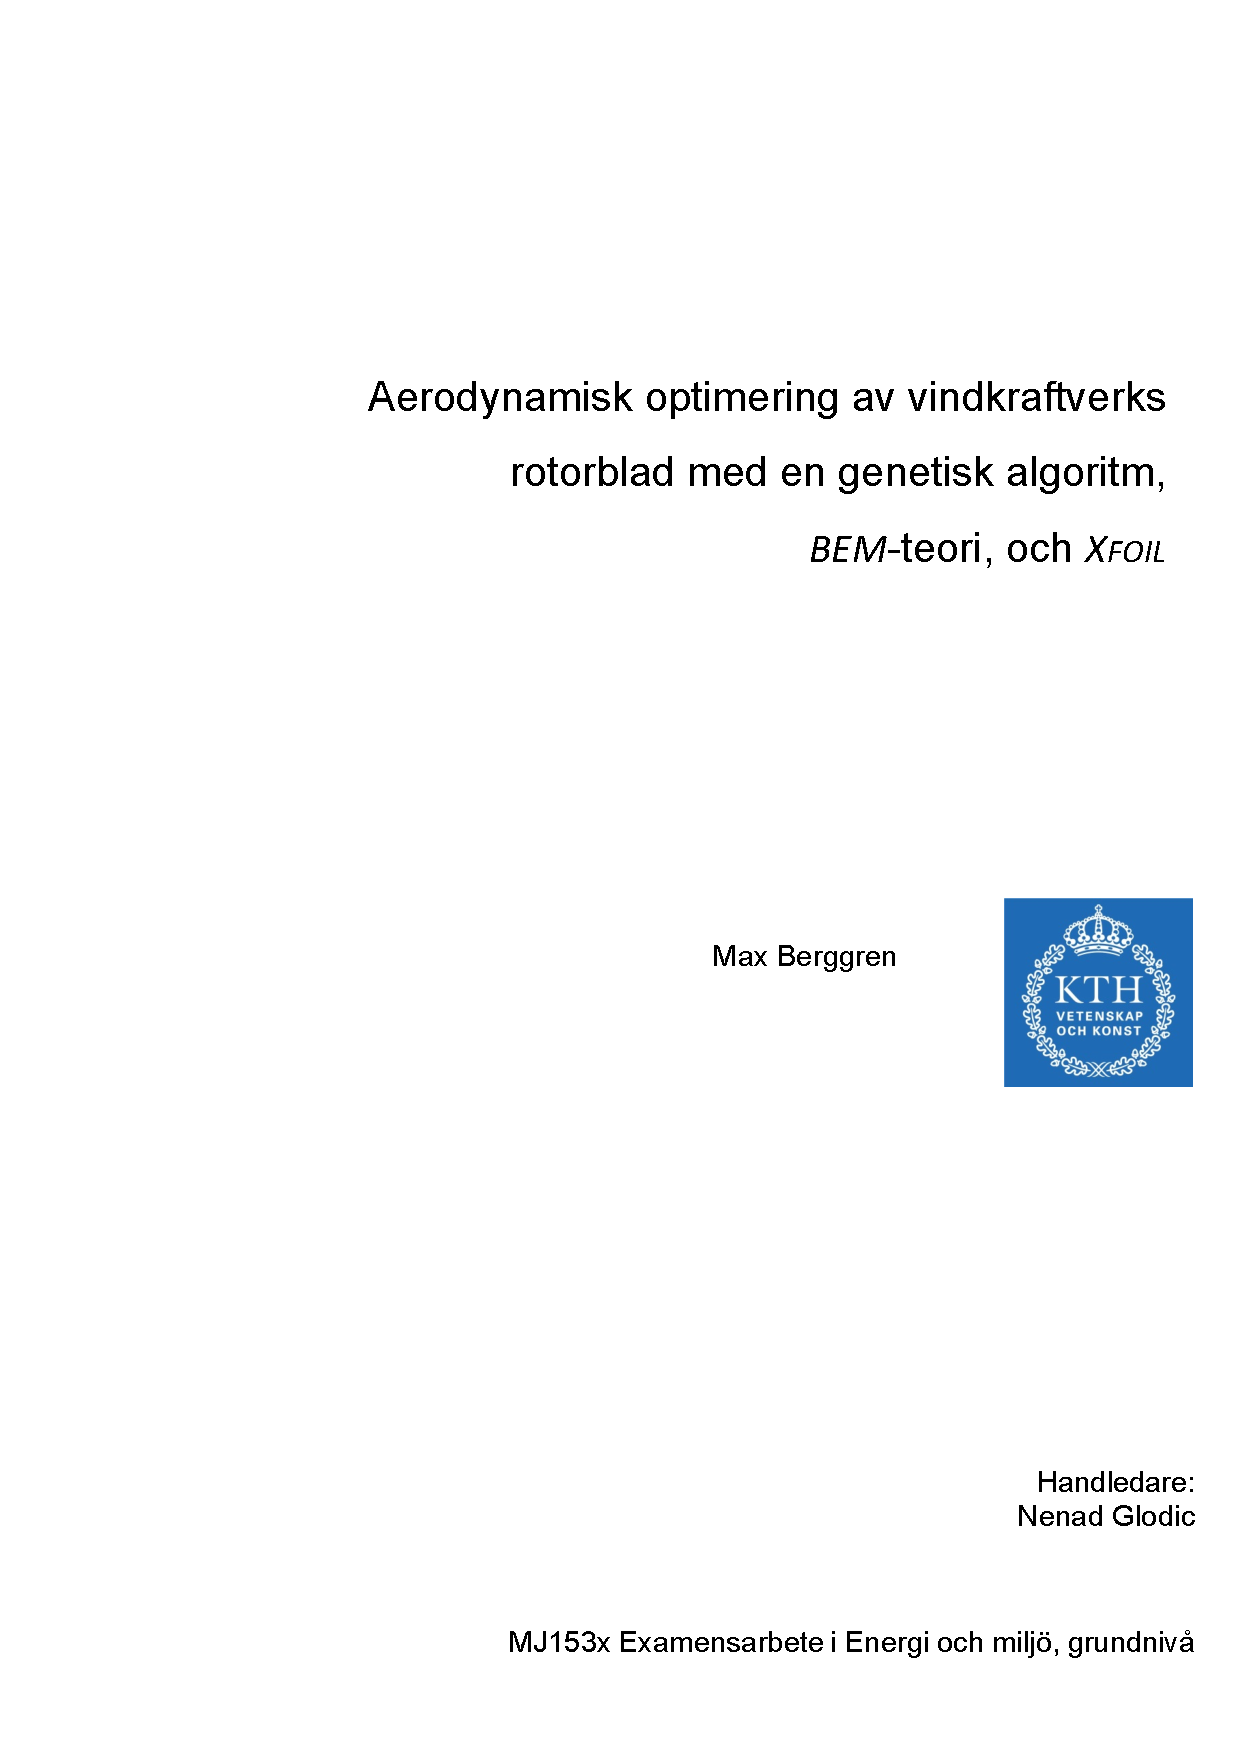
\includepdf[pages={1}]{forsattsblad}
\frontmatter

\begin{comment}
    
    %\end{split}
    
    \title      {Aerodynamisk optimering av ett rotorblad med BEM-teori, genetisk algoritm och Xfoil}
    \authors    {\texorpdfstring
                 {\href{mailto:maxberggren@gmail.com}{Max Berggren}}
                 {Max Berggren}
                }
    \addresses  {\groupname\\\deptname\\\univname}
    \date       {\today}
    \subject    {}
    \keywords   {}
    \maketitle
\end{comment}

\addcontentsline{toc}{chapter}{Sammanfattning}
\begin{abstract}\noindent\begin{quotation}\noindent\small\begin{center}\textbf{ABSTRACT}\smallskip\end{center} This study presents a methodology that enables the annual average power of a wind turbine to be increased by automatically optimizing it's airfoil, twist and chord distribution. As a part of the study the software SiteOpt has been developed. This software connects the open source software XFOIL with the blade element momentum theory. XFOIL gives lift and drag coefficients which enable the blade element momentum theory to predict the power of a wind turbine at different wind and rotational speeds. An optimization algorithm of the type genetic algorithms is used to develop a new rotor blade. An academic benchmark case (Unsteady Aerodynamics Experiment Phase III) was selected as a starting point of the optimization because wind tunnel data was available for that campain. With the geometry developed by the genetic algoritm a theoretical increase of  15 \% more power could be extracted. However, it has been shown that the model has shortcomings at high wind speeds where the predicted power does not match wind tunnel data. This is thought to be related to that the model assumes a completely rigid blade. In real world applications a rotorblade will bend on higher wind speeds (about 8 m/s). It is therefore concluded that the model in its current form is flawed and that future work should aim to take these effects into account. However, a wind histogram for a specific location was used in order to calculate the annual average power for the wind turbine. The wind histogram used in this study to obtain the results has it's wind speeds 81 \% before 10 m/s where the model is acceptable. Therefore the results are largely to be considered accurate. \\ \\ \\ \\ \\ \\ \\ \\ \\ \\ \\ \\ \\ \\ \\ \\ \\ \\ \\ \\ \end{quotation}



\begin{quotation}\noindent  \\ \\ \\ \\ \\ \small\begin{center}\textbf{SAMMANFATTNING}\end{center}\smallskip I denna studie presenteras en metod som möjliggör att ett vindkraftverks årliga genomsnittseffekt kan ökas genom att vingprofiler, korda- och twistdistributioner automatiskt optimeras. För studien har därför programvaran SiteOpt utvecklats. Denna sammanbinder den öppna programvaran XFOIL med den så kallade ``blade element momentum''-teorin. XFOIL kan för vingprofiler ta fram lyft- och motståndskoefficienter vilka möjliggör för ``blade element momentum''-teorin att ta fram ett vindkraftverks effekt vid olika vindhastigheter och rotationshastigheter. En optimeringsalgoritm av typen genetiska algoritmer har använts för att utifrån ett referensfall ta fram ett optimerat rotorblad. I detta fallet valdes ett akademiskt vindkraftverk (Unsteady Aerodynamics Experiment Phase III) där vindtunneldata fanns tillgänglig. Genom att den genetiska algoritmen optimerade vingprofilens geometri kunde teoretiskt 15 \% mer effektuttag göras och en ny vingprofil presenteras i studien. Däremot har det visats att den för studien utvecklade modellen har avvikelser från verkligheten vid höga vindhastigheter. Detta tros ha att göra med att modellen förutsätter ett helt stelt blad, medans verkligheten ofta medför blad som böjer sig vid höga vindhastigheter (c:a 8 m/s). Det konstateras därför att modellen i sin nuvarande form har vissa brister och att framtida arbete bör inrikta sig på att ta hänsyn till dessa hållfasthetsaspekter. Däremot används ett vindhistogram för en specifik plats för att beräkna ett vindkraftverks årliga genomsnittseffekt. Då vindhistogrammet som godtyckligt användes har vindhastigheter som till 81 \% ligger innan 10 m/s, konstateras det att resultatet som presenteras till stor del ändå är giltigt då det använder den delen av modellen som visats ge god överensstämmelse med verkligheten.
\end{quotation}\end{abstract}

\addcontentsline{toc}{chapter}{Innehållsförteckning}
\tableofcontents
\listoffigures
\addcontentsline{toc}{chapter}{Figurlista}
\listoftables
\addcontentsline{toc}{chapter}{Tabellista}



\printnomenclature





\mainmatter
%% ----------------------------------------------------------
%% -------------------------------------------------------------
%% Introduction.tex
%% -------------------------------------------------------------
\chapter{Introduktion} \label{Chapter:Introduction}

Fossila bränslen står idag för 82 \% av världens totala energibehov \citep{Fossila}. Eftersom förbränningen av fossila bränslen är huvudanledningen till växthuseffekten behövs alternativa energikällor. Därför står vindkraft idag för en allt växande global trend av installerad kapacitet vilket syns i \fref{installerad vindkraft}.

\begin{figure}[!htb]
  \centering
  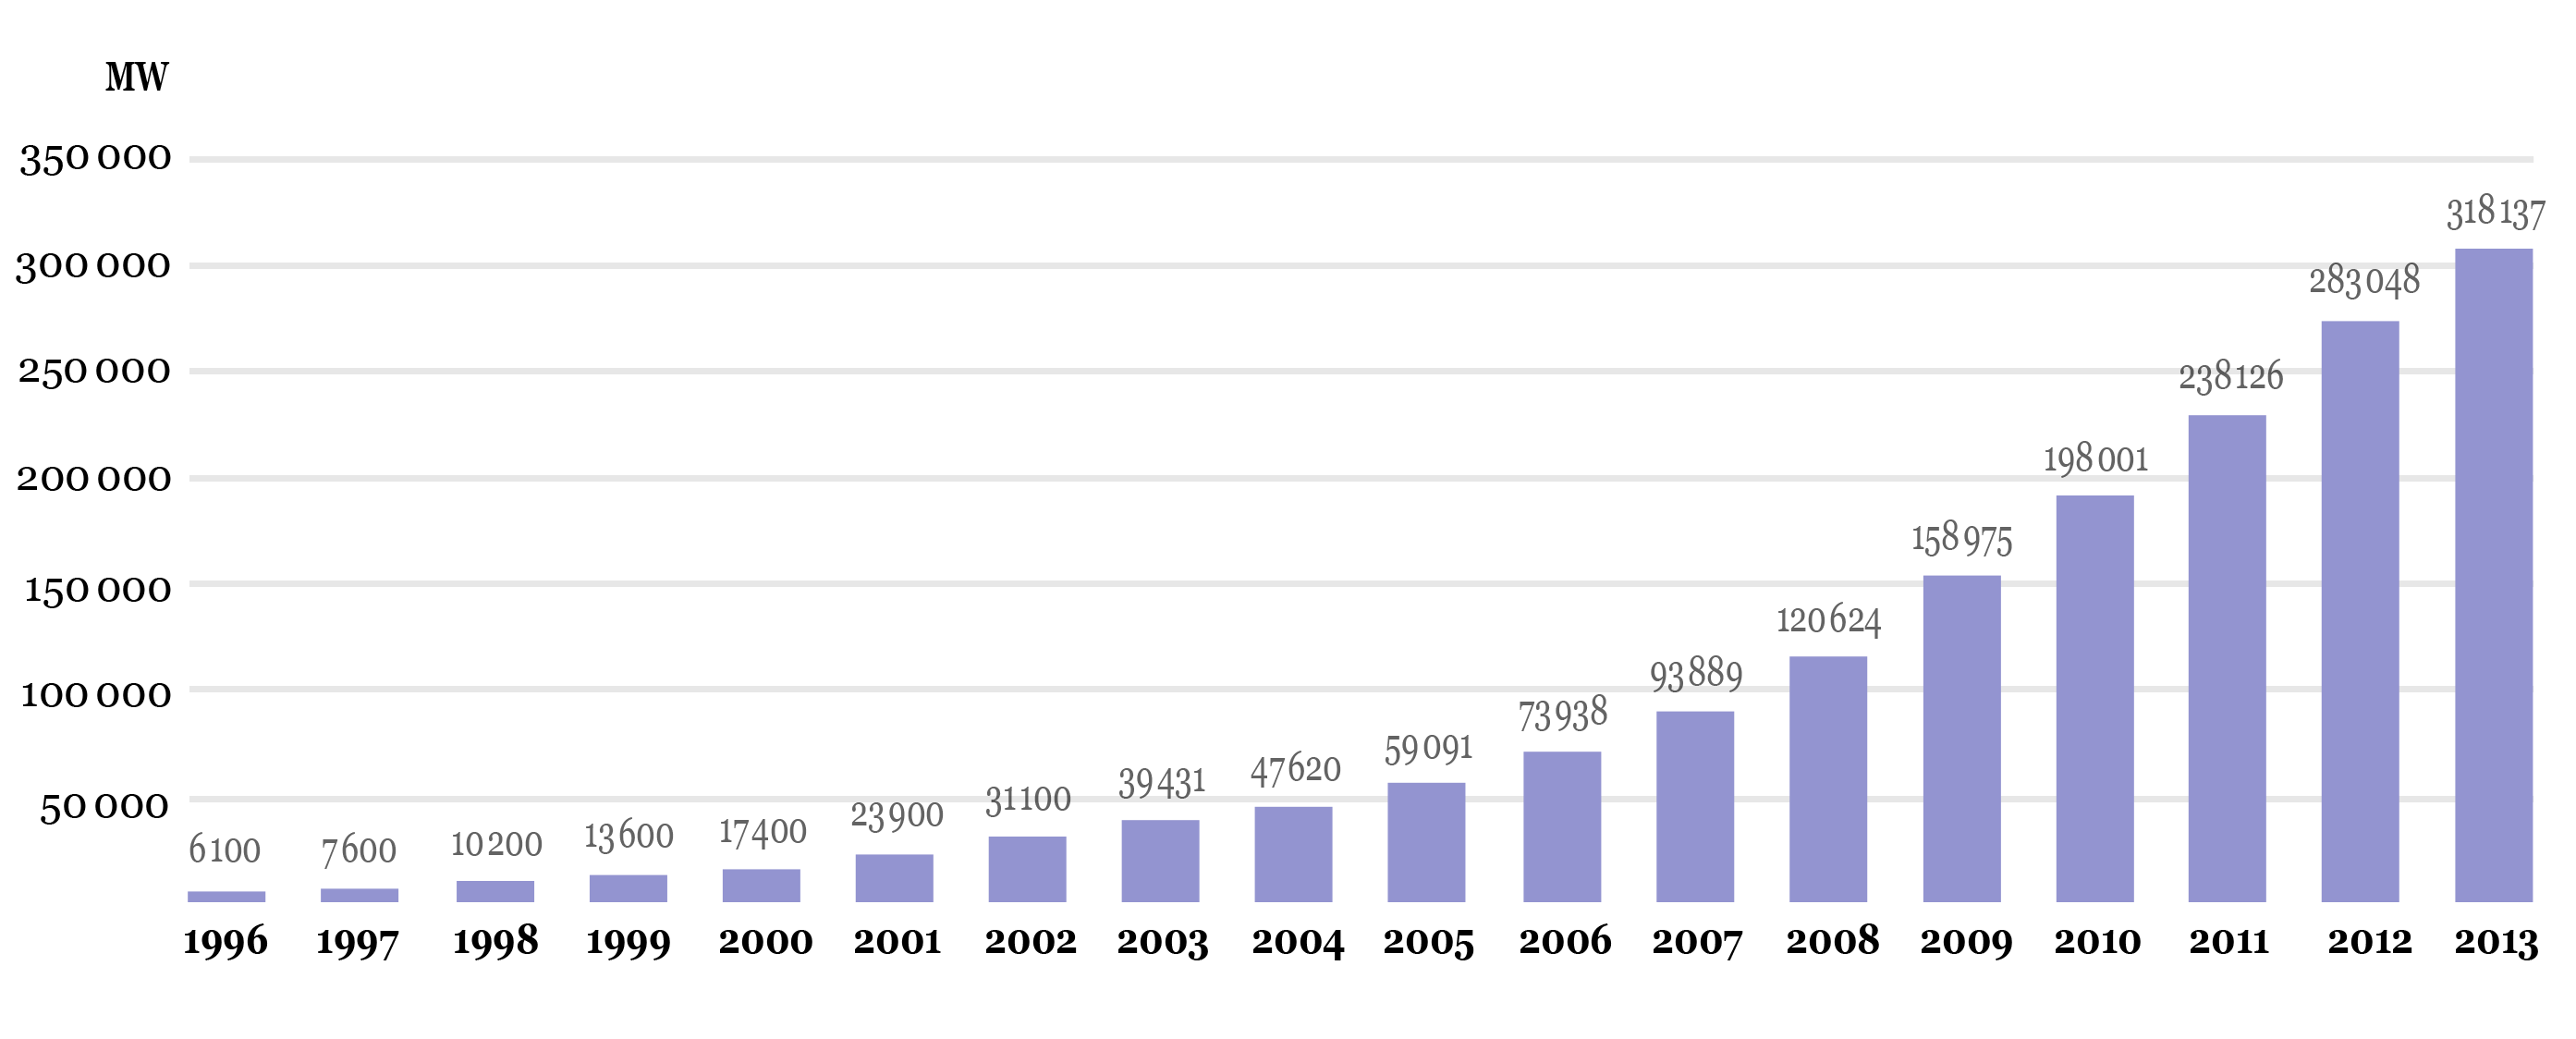
\includegraphics[width=0.9\textwidth]{installeradvind}
  \caption{Totalt installerad global vindkraftseffekt. Reproducerat från \citet{ackvind}.}
  \label{installerad vindkraft}
\end{figure}

Förnyelsebara energikällor såsom vindkraftverk är ideala eftersom de inte medför betydande utsläpp av växthusgaser. Vindkraftverk är samtidigt idag ett av de absolut mest kostnadseffektiva sättet att producera energi. Koldixoxidutsläppen som produktionen och uppförandet av ett vindkraftverk ger upphov till är uppvägda efter tre till sex månader efter att vindkraftverket tagits i drift. Efter detta återstår c:a 20 års fossilfri kraftproduktion vilket är en vanlig livstid för ett vindkraftverk \citep{GWEC}. 

\begin{comment}
\rework{Dock är vindkraft, likt alla andra kraftkällor - förknippat med sina negativa sidor. Energi kan endast produceras när vinden blåser vilket leder till att energi då måste komma från andra energikällor. När istället det motsatta råder, ett överskott på vindenergi - måste energin lagras eller transporteras vidare till där den behövs. Andra nackdelar är störande ljud som de ger upphov till, skuggor som sveper, elektromagnetisk strålning och fåglar och fladdermöss som dör i kollisioner med rotorbladen. Dessa nackdelars betydelse har med åren minskat eftersom lösningar finns på många av dem, och trots nackdelarna - överväger de positiva effekterna. [Ska nog bort]}
\end{comment}

\begin{comment}
Installerad effekt växer

Tyskland fasar ut efter Fukushima. Till 2020 ingen kärnkraft.

Vindkraftens nackdelar. Endast när det blåser.Oljud. Viosuellt. Skuggor som flimmrar. Djur som dör. Går att göra något åt och problemen minskar succesivt. Positivt överväger det negativa.
\end{comment}


\section{Syfte}
För att gynna möjligheterna till en hållbar framtid syftar denna studie bidra till effektiviseringar av ett vindkraftverks energiproduktion.
%men även främja öppenhet och vindlighet av information.

\section{Mål}
Det generella målet är att utifrån ett histogram med vindhastigheter för en plats kunna presentera det rotorblad som ger största genomsnittliga effekt för ett vindkraftverk. Detta kommer ske genom ett par delmål:

\begin{itemize}

  \item Skapa en modell som förutsäger ett vindkraftverks genomsnittliga effekt.

  \item Hitta och presentera ett referensfall som kan användas för att utvärdera den skapade modellens giltighet.
  
  \item Ett optimeringsproblem ska formuleras och implementeras som kommunicerar med modellen för att hitta rotorblad med högre genomsnittlig effekt.
  
  \item Ta fram ett alternativt rotorblad genererat ur optimeringen och jämföra dess prestanda mot referensfallet.
 
\end{itemize}




\section{Litteraturstudie}

\subsection{Vindturbiner}
Vindkraftverk är en maskin som konverterar vindens inneliggande rörelseenergi till elektrisk energi. Detta görs genom att inkommande luft skapar en lyftkraft på rotorbladets vingprofil som driver ett vridmoment. Vridmomentet utnyttjas sedan i en generator för att producera el. I \fref{liftdrag} syns ett tvärsnitt av ett vindkraftverks rotorblad med lyft- ($L$) och motstånds- ($D$) och normalkraft ($N$) utmarkerat. 

    \begin{figure}[!htb]
      \centering
      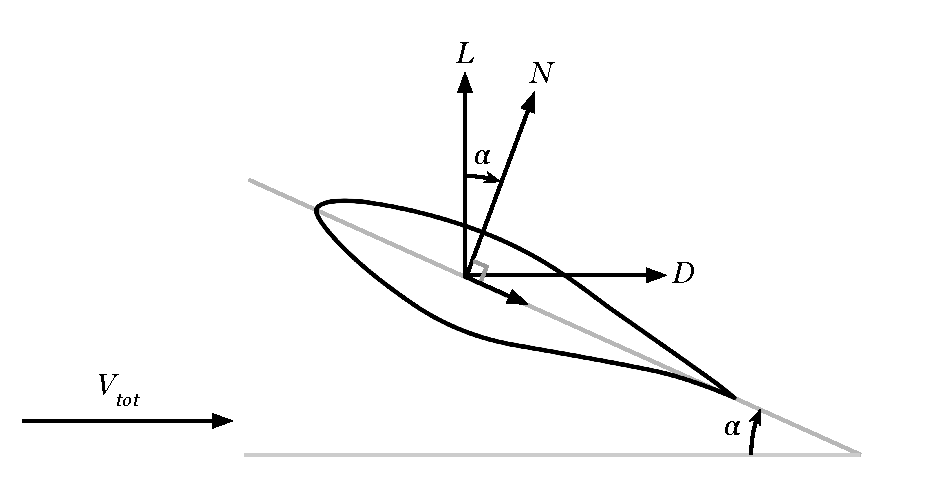
\includegraphics[width=0.9\textwidth]{liftdrag.pdf}
      \caption{Vingprofil med krafter utmarkerat.  Fritt reproducerat från \citet{hansen}.}
      \label{liftdrag}
    \end{figure}

\begin{figure}[!htb]
  \centering
  \subfigure[Horizontellt axlad vindturbin (\textsc{hawt})]{
    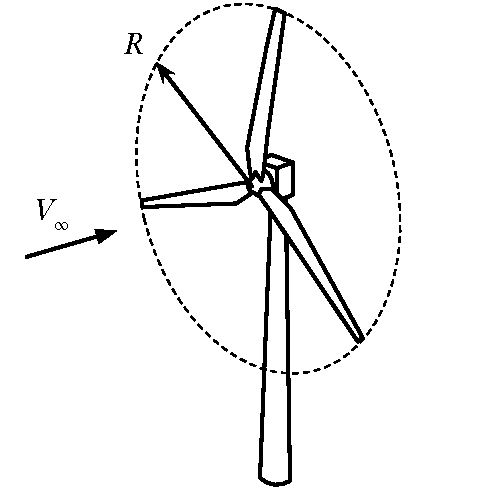
\includegraphics[height=7cm]{hawt.pdf}
    \label{hawt}
  }
  \subfigure[Vertikalt axlad vindturbin (\textsc{vawt})]{
    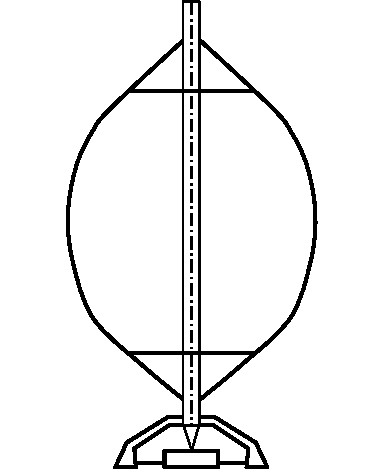
\includegraphics[height=7cm]{vawt.pdf}
    \label{vawt}
  }
  \caption{De två vanligaste typerna av vindturbiner. Fritt reproducerat från \citet{wehb}.}
  \label{hawtvawt}
\end{figure}


I \fref{hawt} syns den horisontellt axlade vindturbinen (ofta kallat \textsc{hawt}) vilken är den vanligast förekommande. En alternativ variant på vindkraftverk är den vertikalt axlade vindturbinen (\textsc{vawt}) som syns i \fref{vawt}. Dessa har fördelarna att de producerar effekt oavsett vindriktning samt att de är lättare att utföra service på då viktiga delar nås från fundamentet. Dessa utvecklades i kommersiell skala fram till 80-talet men får idag mindre uppmärksamhet på grund av dess nackdelar:

    \begin{itemize}
    
      \item Närmast marken är vindhastigheten lägre (vidhäftningsvilkoret) vilket gör att turbinens nedre del är mindre effektiv än den övre.
    
      \item Turbinen har svårt att självstarta och behöver därför en motor för att komma upp i en hastighet där de producerar effekt.
      
      \item Vridmomentet fluktuerar mycket mellan rotationerna.
      
      \item De kräver en mekanisk broms vid höga vindhastigheter för att inte komma upp i rotationshastigheter där konstruktionen går sönder.
     
    \end{itemize}


\textsc{hawt} är den idag mest förekommande varianten och den enda som behandlas i denna uppsats. I stora drag består en \textsc{hawt} av en motorgondol monterat på ett högt torn. I motorgondolen finns en generator samt även ofta ett växelhus, även om ett ökande antal vindturbiner idag är utan växelhus. För att vända turbinen mot den inkommande vinden finns oftast en motor som möjliggör gir ($\gamma$) (se \fref{gir}). 

\begin{figure}[!htb]
  \centering
  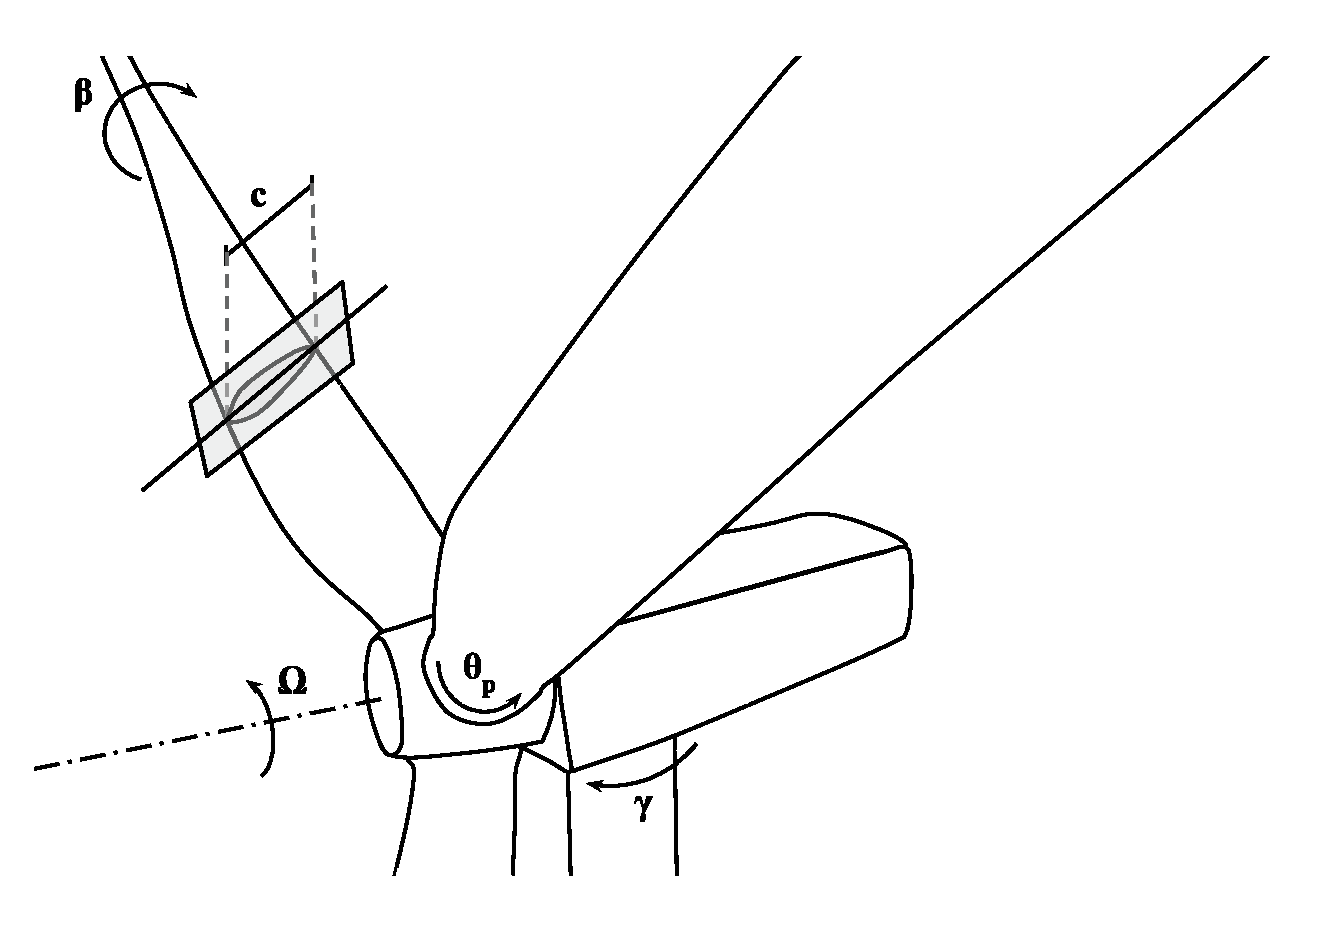
\includegraphics[width=12cm]{gir.eps}
  \caption{Gir ($\gamma$), korda ($c$) och pitch ($\theta_p$)  utmarkerat på en vindturbin.}
  \label{gir}
\end{figure}

En rotor som sitter framför motorgondolen uppströms vindens riktning samt tre rotorblad är idag den vanligast förekommande typen av vindturbin i kommersiell drift. Vanligast är även att rotationshastigheten ($\Omega$) är variabel.

För att kunna kontrollera vindkraftverket vid höga rotationshastigheter sitter ofta även motorer som kontrollerar rotorbladens så kallade pitch ($\theta_p$). När vindhastigheten blir för hög kan rotorbladen ställas så att lyftkraften minskar och på så sätt hålla generatorn från att skadas. Korda ($c$) beskriver rotorbladets vingprofils längd i ett tvärsnitt och varierar ofta med radien. Dessa koncept illustreras i \fref{gir}. En ytterligare vridning längs radien kallas \emph{twist} ($\beta$) och definieras som avvikelse från kordans plan i rotorbladets topp.

Idag existerar vindturbiner med maximal effekt från några enstaka kW till flera MW och rotordiametern är därefter. Ett vindkraftverk i MW-klass är inte sällan över 100 m i diameter \citep{kap10}.

\subsection{Vindens inneliggande energi}
Vindens inneliggande kinetiska energi som passerar den cirkulära area rotorn sveper i \fref{hawt} kan visas ge effekten

\begin{equation}\label{pvind} P_{vind} = \frac{1}{2}\rho A V_{\infty}^{3}  =  \frac{1}{2}\rho V_{\infty}^{3}\pi R^2 \end{equation}

Där $A$ är den cirkulära arean $\pi R^2$ där $R$ är radien och $V_\infty$ vindhastigheten uppströms rotorn. Ekvationen visar alltså att energin som kan tas ut ur vinden beror på vindhastigheten i kubik vilket är viktigt att komma ihåg. Den visar även att effektuttaget är beroende på radien i kvadrat, vilket förklarar dagens trend med ökande storlek på vindkraftverken.

I praktiken är effekten som ett vindkraftverk genererar aldrig så hög som ekvation \ref{pvind} antyder. Det hade inneburit att vinden tappat all sin hastighet genom rotorn och blockerat ytterligare vind. Detta leder oss till den dimensionslösa storheten $C_P$ som är vanlig i dessa sammanhang definierad

\begin{equation}\label{cp} C_P =  \frac{P}{P_{vind}} = \frac{P}{\frac{1}{2}\rho V_{\infty}^{3}\pi R^2} \end{equation}

Detta är alltså andelen producerad effekt mot det som annars hade passerat den cirkulära arean.

Nästa vanliga storhet att vara bekant med är löptalet $\lambda$ (på engelska tip speed ratio) vilket $C_P$ visar sig vara starkt beroende av. Denna definieras

\begin{equation}\label{tsr} \lambda = \Omega R / V_\infty = V_{topp}/V_\infty \end{equation}

Vilket relaterar rotorns toppars hastighet $\Omega R$ mot den inkommande friströmshastigheten $V_\infty$. $\lambda$ brukar vara mellan 7 och 10 när vindkraftverk producerar maximalt $C_P$. 

Den tredje dimensionslösa enheten är Reynolds tal som i vindkraftssammanhang definieras

\begin{equation}\label{reynolds} Re = V_{total} c/\nu \end{equation}

$V_{total}$ kommer att definieras tydligare i \ref{BEMlitt} men är den totala hastigheten en vingprofil ser när både inkommande hastighet $V_\infty$ och $\lambda$ gör sig gällande. $c$ betecknar kordan och $\nu$ luftens kinematiska viskositet. 

\subsection{Effekt-kurvan för ett vindkraftverk}

I \fref{vestas} visas en Vestas V80 2 MW vindkraftverks effektkurva. Detta är ett vindkraftverk med 80 meter i diameter och med en typisk effektkurva. Inkoppling sker när lägsta vindhastighet som kan producera effekt uppnås $U_{in}$ (på engelska \emph{cut-in wind speed}), vilket i detta fallet är 3 m/s.  

\begin{figure}[!htb]
  \centering
  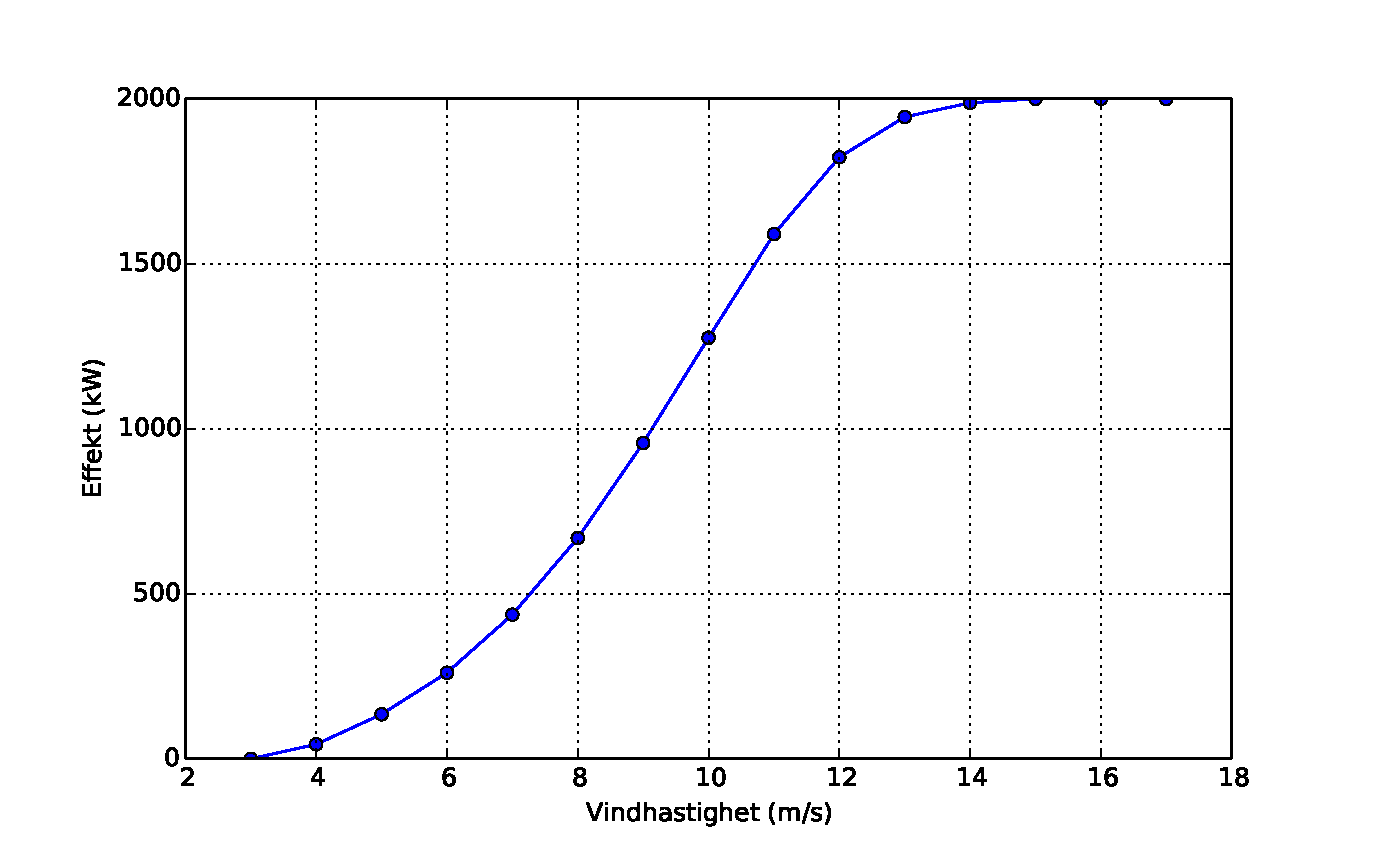
\includegraphics[width=11cm]{powerwindspeed.eps}
  \caption{Effektkurva för Vestas V80 2 MW 80 m diameter. Fritt reproducerat från \citet{smallwindturbines}.}
  \label{vestas}
\end{figure}

Effekten planar i \fref{vestas} ut mot det som kallas märkeffekt (på engelska \emph{rated power}) vilket är det maximala effekt generatorn kan producera. När denna effekt närmas vrids rotorbladen via deras pitch ($\theta_p$) för att minska lyftkraften och på så vis kunna hålla sig under märkeffekten. Alternativt används en mekanisk broms. Detta görs för att generatorn inte ska skadas.

Vid en maximal vindhastighet $U_{ut}$ kommer även vindkraftverket att stänga av helt och hållet (eng: \emph{cut-out speed}) eftersom risken för skador från den höga rotationshastigheten och dess medförda centrifugalkrafter då är för stora. Detta kan göras genom att bladen ställs så att endast motståndskraft uppstår vilket får rotationen att upphöra. 

\pagebreak
\subsection{$C_P$-kurvan}

En kurva visandes $C_P$ mot $\lambda$ visas i \fref{cpTSR}. Som tidigare nämnt finns alltid ett löptal $\lambda$ där ett maximalt $C_P$ uppnås. Därför körs moderna vindkraftverk med variabel hastighet för att kunna följa detta maximum.

\begin{figure}[!h]
  \centering
  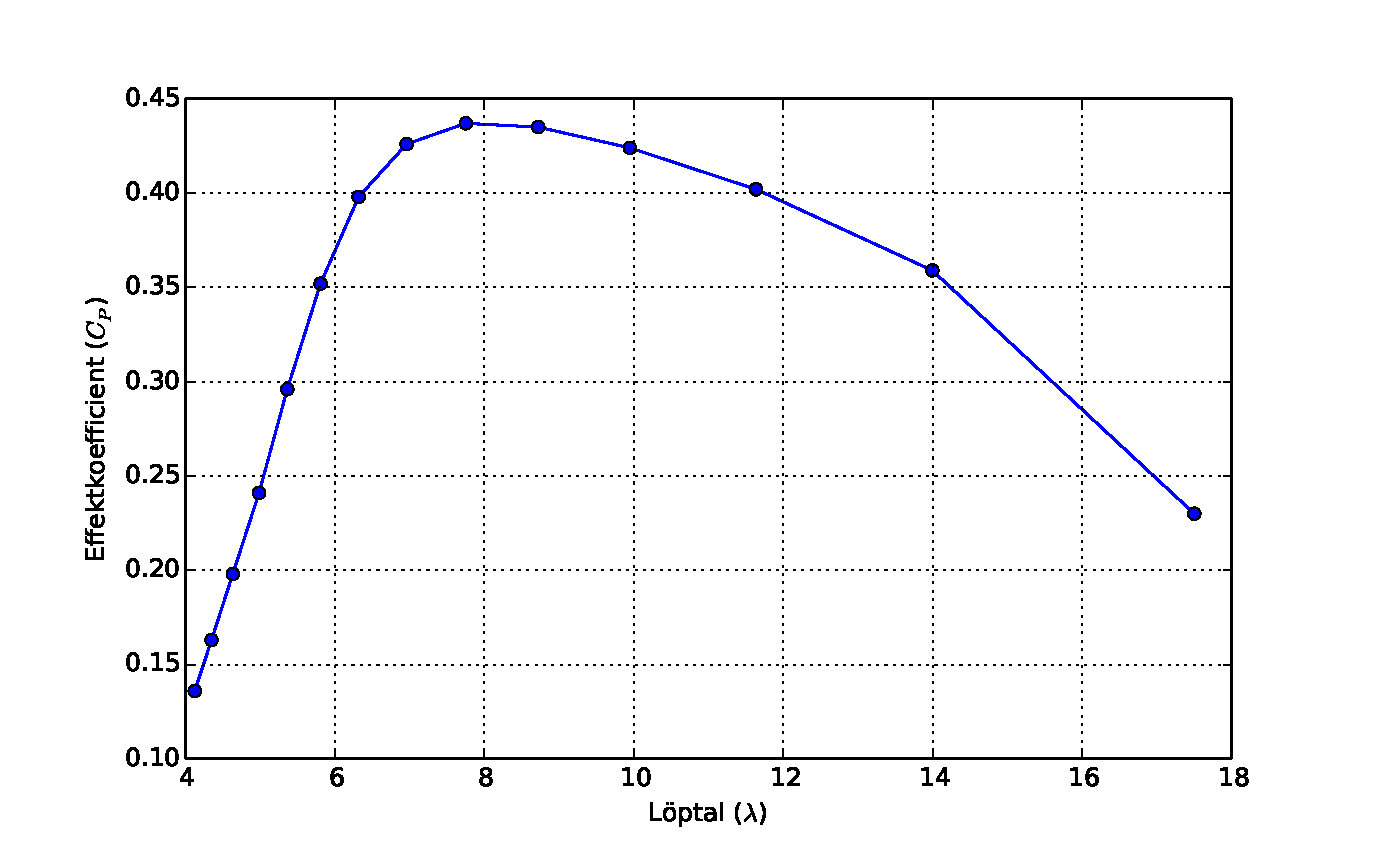
\includegraphics[width=11cm]{cpTSR.eps}
  \caption{$C_P$ mot $\lambda$ för Vestas V80 2 MW 80 m diameter. Fritt reproducerat från \citet{smallwindturbines}}
  \label{cpTSR}
\end{figure}

\pagebreak
\subsection{$C_l$- och $C_d$-kurvor}
\label{ClochCdkurvor}


$C_l$ och $C_d$ är på samma vis som tidigare en dimensionslös en storhet som beskriver lyftkraft och motståndskraft för en tvådimensionell vingprofil. Dessa definieras på följande sätt

\begin{equation}\label{c_l}
\begin{array}{cc}
C_l = \frac{l}{\frac{1}{2}\rho V_{tot}^2   c}, & C_d = \frac{d}{\frac{1}{2}\rho V_{tot}^2   c} \\ 
\end{array}
\end{equation}


Där $C_l$ och $C_d$ kommer visa sig beroende på vingprofilens utformning, $\alpha$ och $Re$. Typiska kurvor för deras starkaste beroende $\alpha$ visas i \fref{ClCd}. Här syns att vid ett speciellt $\alpha$ har $C_l$ nått sitt maximum och börjar minska. Detta kallas stall-vinkeln och kommer vidare benämnas $\alpha_{stall}$. 

\begin{figure}[!h]
  \centering
  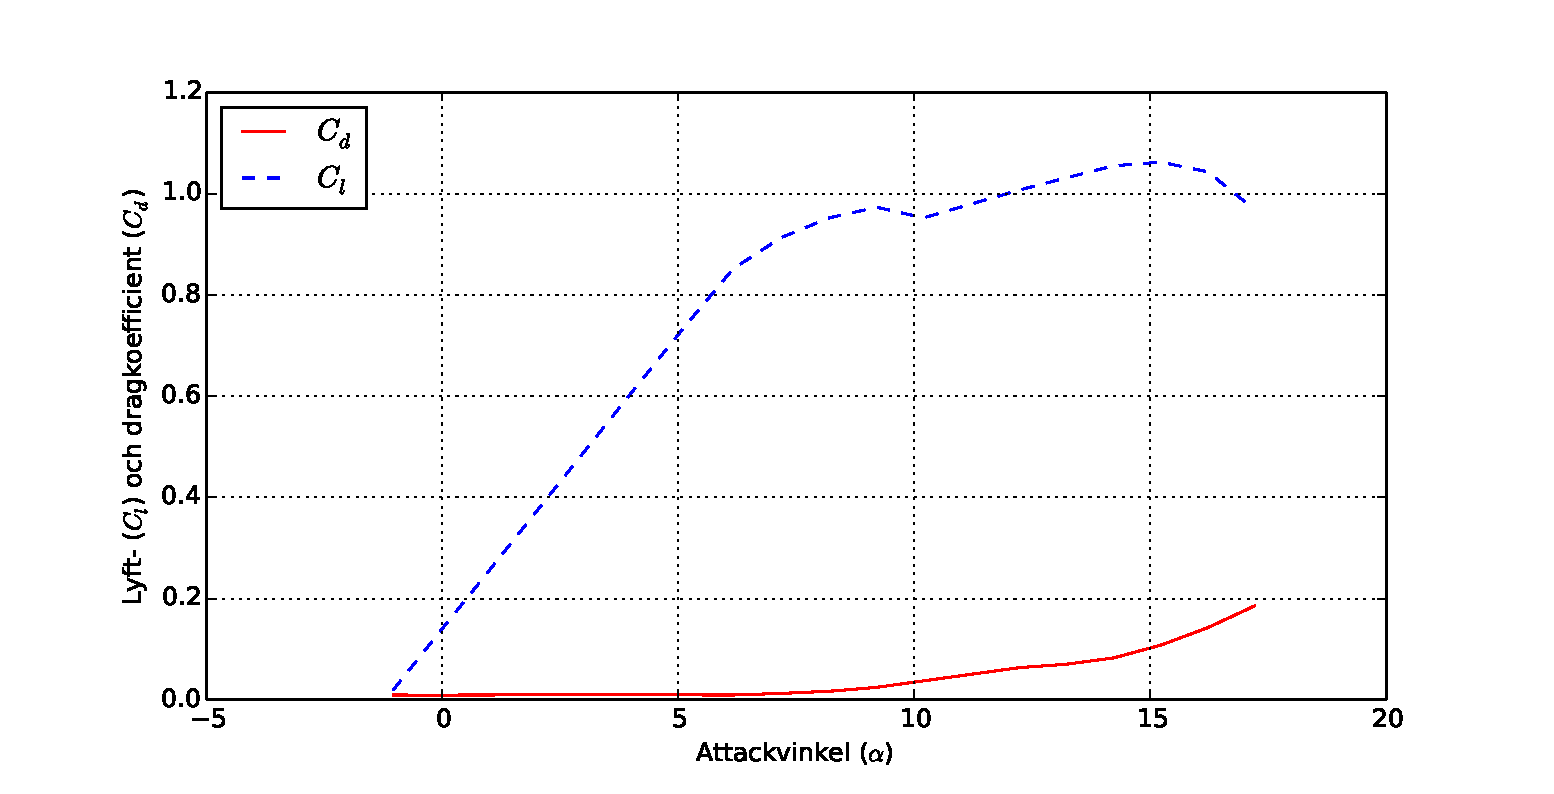
\includegraphics[width=12cm]{S809_Alfa_Cl_Cd}
  \caption{$C_l$ och $C_d$ för vingprofilen S809 vid $Re$ en miljon. Data från \citet{s809data}}
  \label{ClCd}
\end{figure}


Ekvationer som nu presenterats återfinns i mer utförlig form i \citet{smallwindturbines}. 



\subsection{Programvaror och erhållande av $C_l$ och $C_d$}
Lyft- och motståndskoefficient ($C_l$ och $C_d$) är de aerodynamiska variabler som är av högst intresse för att kunna göra en \textsc{Bem}-analys. Att ta fram dessa i vindtunnelexperiment är dock omöjligt i en optimeringsstudie som då hade inneburit att tusentals vingprofiler skulle byggas och testas i tunneln.

\textsc{cfd} (Computional Fluid Dynamics) är ett alternativ som ger resultat av hög kvalitet, men är ofta väldigt beräkningsintensivt. \cite{Xfoil} har utvecklat programvaran \textsc{Xfoil} som kan lösa det inviskösa och viskösa flödet kring en vingprofil. Detta genom en linjär vorticitetsmetod tillsammans med Karman-Tsien-kompesibilitetskorrektion löses det inviskösa flödet. Gränsskiktet och övergången till turbulent flöde löses simultant med det inviskösa potentialflödet med en global Newton–Raphson-metod.

Flertalet studier har undersökt \textsc{Xfoil}s giltighet och kunnat konstatera god överensstämmelse med verkligheten vid låga $\alpha$ \citep{CST, XfoilVerifikation}. \textsc{Xfoil} avviker enligt \citet{XfoilVerifikation} från experimentella resultat för $C_l$ nära och efter stallvinkeln passerats där $C_l$ då överskattas. Vid höga vinklar konstateras även att \textsc{Xfoil} underskattar $C_d$ och en korrektionsfaktor där \textsc{Xfoil} data ökas 10 \% används. Dock skulle inte denna korrektionsfaktor räcka till för att kompensera avvikelsen för $C_d$ som presenteras i \citet{CST}.


\subsection{Val av modell för att förutsäga ett vindkraftverks produktion}

Strömningen som uppstår kring ett vindkraftverks rotorblad är ofta av transient natur, turbulent, tredimensionellt samt med många separationer i flödet. Detta gör det till ett komplext problem som är väldigt tidsödande att lösa med \textsc{cfd} (Computional Fluid Dynamics). Ett alternativ till \textsc{cfd} är potentialteori, men då kan ingen hänsyn till fluidens viskositet tas. Därför har det blivit industristandard att idag använda ``blade element momentum''-teori (\textsc{Bem}). Detta är en tvådimensionell metod som i princip extrapoleras in i tre dimensioner tillsammans med semi-empiriska antaganden som kommer från jämförelser med \textsc{cfd}-studier. Detta leder till en metod som till väldigt låg beräkningskostnad kan ge tillräckligt goda förutsägelser på ett vindkraftverks elproduktion. \textsc{Bem}s största nackdel är att den inte tar hänsyn till vindens transienta natur utan förutsätter ett flöde i samma hastighet oberoende av tiden (stationärt tillstånd) samt en hastighet oberoende av position i rymden \citep{Qblade}. 

I \citet{bembraelleranus} visas att \textsc{Bem}s största felkälla är dess lyft- och motståndskoefficienter ($C_l$ och $C_d$). \textsc{Bem} kan alltså antas ge ett resultat nära verkligheten givet att lyft- och motståndskoefficienter är korrekta. Korrekta koefficienter kan ges med empiriska mätningar på vingprofiler i en vindtunnel. Tas dessa fram på annan väg bör resultatet för \textsc{Bem} beaktas med försiktighet.



\begin{comment}
\citet{UnsteadyWind} har visat att uppmätta resultat i vindtunnlar kan vara i underkant mot vad som sedan turbinen behöver klara ute i fält på grund av vindens stötvisa natur. Toppbelastningen visade sig vara högre än vad vindtunnelexperiment tillsammans med \textsc{Bem} förutsade vilket är en underliggande orsak till slitage i mekaniska delar som vindkraftverk dras med. 
\end{comment}






\subsection{Vingprofilsrepresentation}

    \begin{figure}[!h]
      \centering
      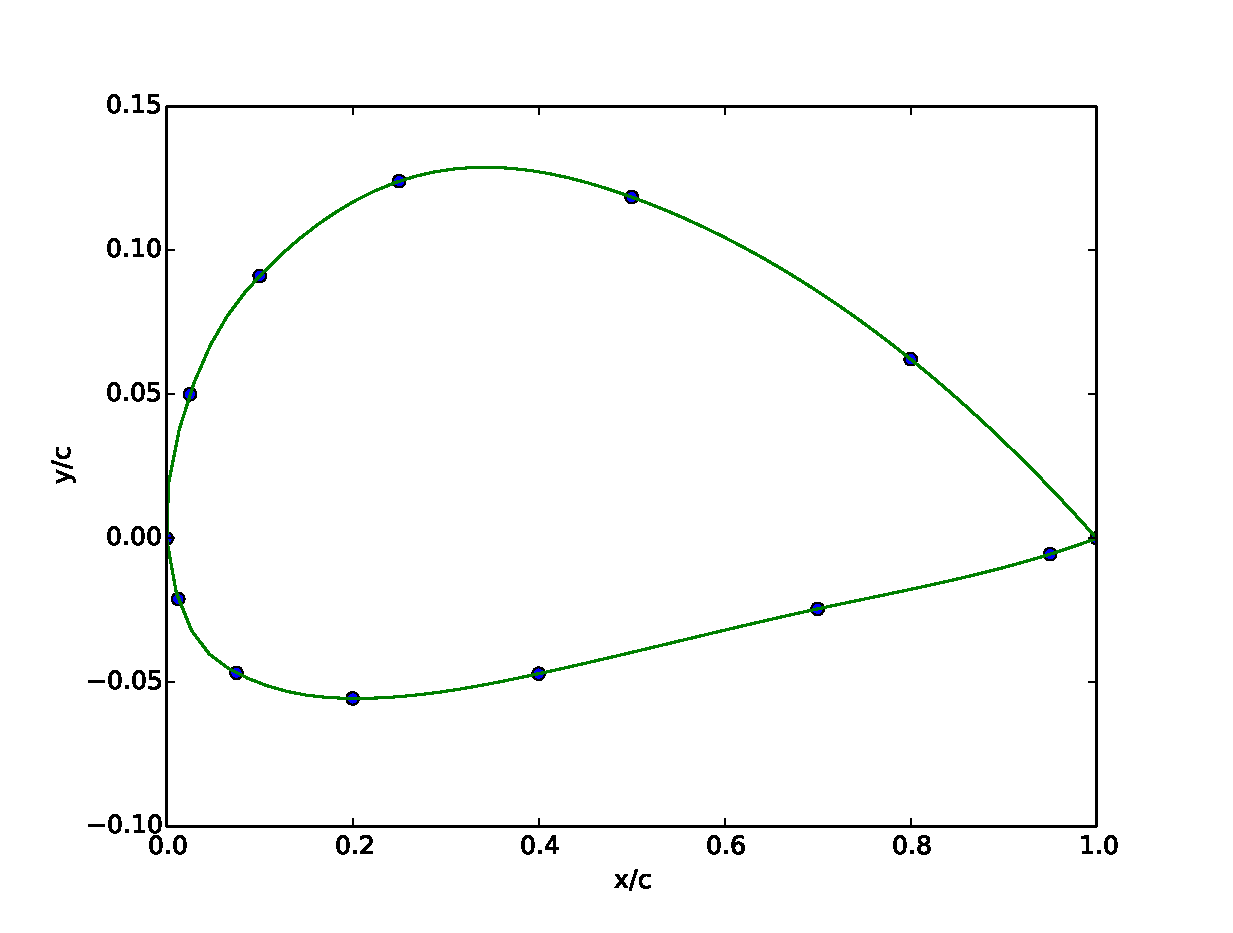
\includegraphics[width=0.7\textwidth]{connectTheDots}
      \caption{Vingprofilsrepresentation genom sammanbindning av diskreta punkter genom B-spline-interpolation}
      \label{connectTheDots}
    \end{figure}

Ett vindkraftverks rotorblad kan anses bestå av flera tvådimensionella vingprofiler. Det går att representera dessa vingprofiler på väldigt många olika sätt. Oftast görs detta med diskreta punkter som sammanbinds med någon interpolationsteknik (se \fref{connectTheDots}). Frihetsgrader benämner antalet parametrar som sedan kan förändras i optimeringsprocessen. En punkt i xy-planet är därmed förknippat med två frihetsgrader när punkten inte är låst i någon led. 

%% Undantaget är när en diskretiseringspunkt låses i x- eller y-ledd.

\citet{DrelaTrubbel} har visat att en allt för detaljerad representation av vingprofilen har många negativa effekter. Dels eftersom beräkningskostnaden växer med antalet parametrar som sedan optimeras över, men även eftersom optimeringen då kan börja ta hänsyn till små fysikaliska fenomen som borde vara obetydliga. I \citet{DrelaTrubbel}  utvecklades en vågformad yta på vingprofilen som uppstod för att kompensera för separationsbubblor. Dock är platsen för där separationsbubblorna uppstår beroende av $C_l$ och därför inte giltig för mer än just en angreppsvinkel på vingprofilen. \begin{comment}\hl{En vingprofil som inte är mjuk är ur tillverkningssynpunkt inte heller lämplig}.\end{comment} \citet{DrelaTrubbel} hade i sin studie 60 frihetsgrader på vingprofilsrepresentationen.

Av ovanstående anledningar används idag ett färre antal diskreta punkter. \citet{5MWkillen} använder som många andra \citep{LowRe,Grasso} bezierkurvor för denna interpolationen. Fördelarna är en mjuk representation av vingprofilen med få parametrar. \citet{5MWkillen} använder här 22 frihetsgrader men ner till 16 används \citep{Grasso}.

Liknande bezierkurvor är B-splines som även de ger en mjuk representation. Största skillnaden är att en förändring i en diskretiseringspunkt ger en mer lokal förändring på kurvan än vad motsvarande gör i en bezierkurva. \citet{Dansken} använder B-splines. 

\citet{Cencelli} har istället valt att definiera fem grundprofiler som sedan mixas efter olika proportioner. Detta inskränker således designrymden men har fördelen att frihetsgraderna minskar.

CST-metoden har i \citet{CST} använts vilket i princip är användandet av ett polynom för representationen. Koefficienterna i polynomet är således frihetsgraderna vilka kan hållas få till bekostnad på att alla vingprofiler inte kan representeras på detta sätt.

Andra författare har valt ytterligare förenklingar där t.ex. \citet{Victoria} valt att endast låta optimeringsalgoritmen välja ur en förutbestämd mängd vindprofiler (NACA 44XX).





\begin{comment}
\subsection{Programmeringsspråk}
Implementering av ett optimeringsproblem likt det studerade kan givetvis göras i vilket programmeringsspråk som helst. Trots det är det stor övervikt för \textsc{MatLab} \citep{CST, Cencelli, 5MWkillen}. \hl{Python används i en studie av de jag arbetat med, men då endast för att kalla på Fortran-rutiner} \citep{Victoria}. %\citet{5MWkillen} använder sig av NREL FAST vilket är en BEM-kod utvecklad i fortran.
\end{comment}

\subsection{``Blade element momentum''-teori (\textsc{Bem})}
\label{BEMlitt}

``Blade element momentum''-teori (\textsc{Bem}) är idag ett vanligt sätt att förutsäga ett vindkraftverks prestanda. Givet pitch-vinkel ($\theta$) och löptal ($\lambda$) kan effekt och tryckkraft uppskattas. För att kunna göra detta används två strömningsmekaniska teorier: Endimensionell rörelsemängdsteori och ``blade element''-teori som i kommande stycken beskrivs i korthet efter hur de formulerats i \citet{hansen}.

\subsubsection{Analys av rörelsemängd i en dimension}
\label{1dmomentumteori}

Denna teori beskriver en förenklad och ideal rotor som kan uppskattas till en cirkulär disk (d.v.s. oändligt antal rotorblad) utan tjocklek där strömningen är friktionsfri och inkompressibel. Det finns heller ingen rotationell hastighetskomponent i vaken bakom rotorn. Disken kommer att stanna upp vindhastigheten $V_{\infty}$ uppströms till $u$ i rotorplanet och till $u_1$ i vaken bakom rotorn. Trycket kommer att från atmosfärstrycket $p_0$ höjas till $p$ direkt innan rotorn för att sedan göra ett diskontinuerligt fall $\Delta p$. Hur tryck och vindhastighet varierar visas i \fref{tryckfall}.

\begin{figure}[!htb]
  \centering
  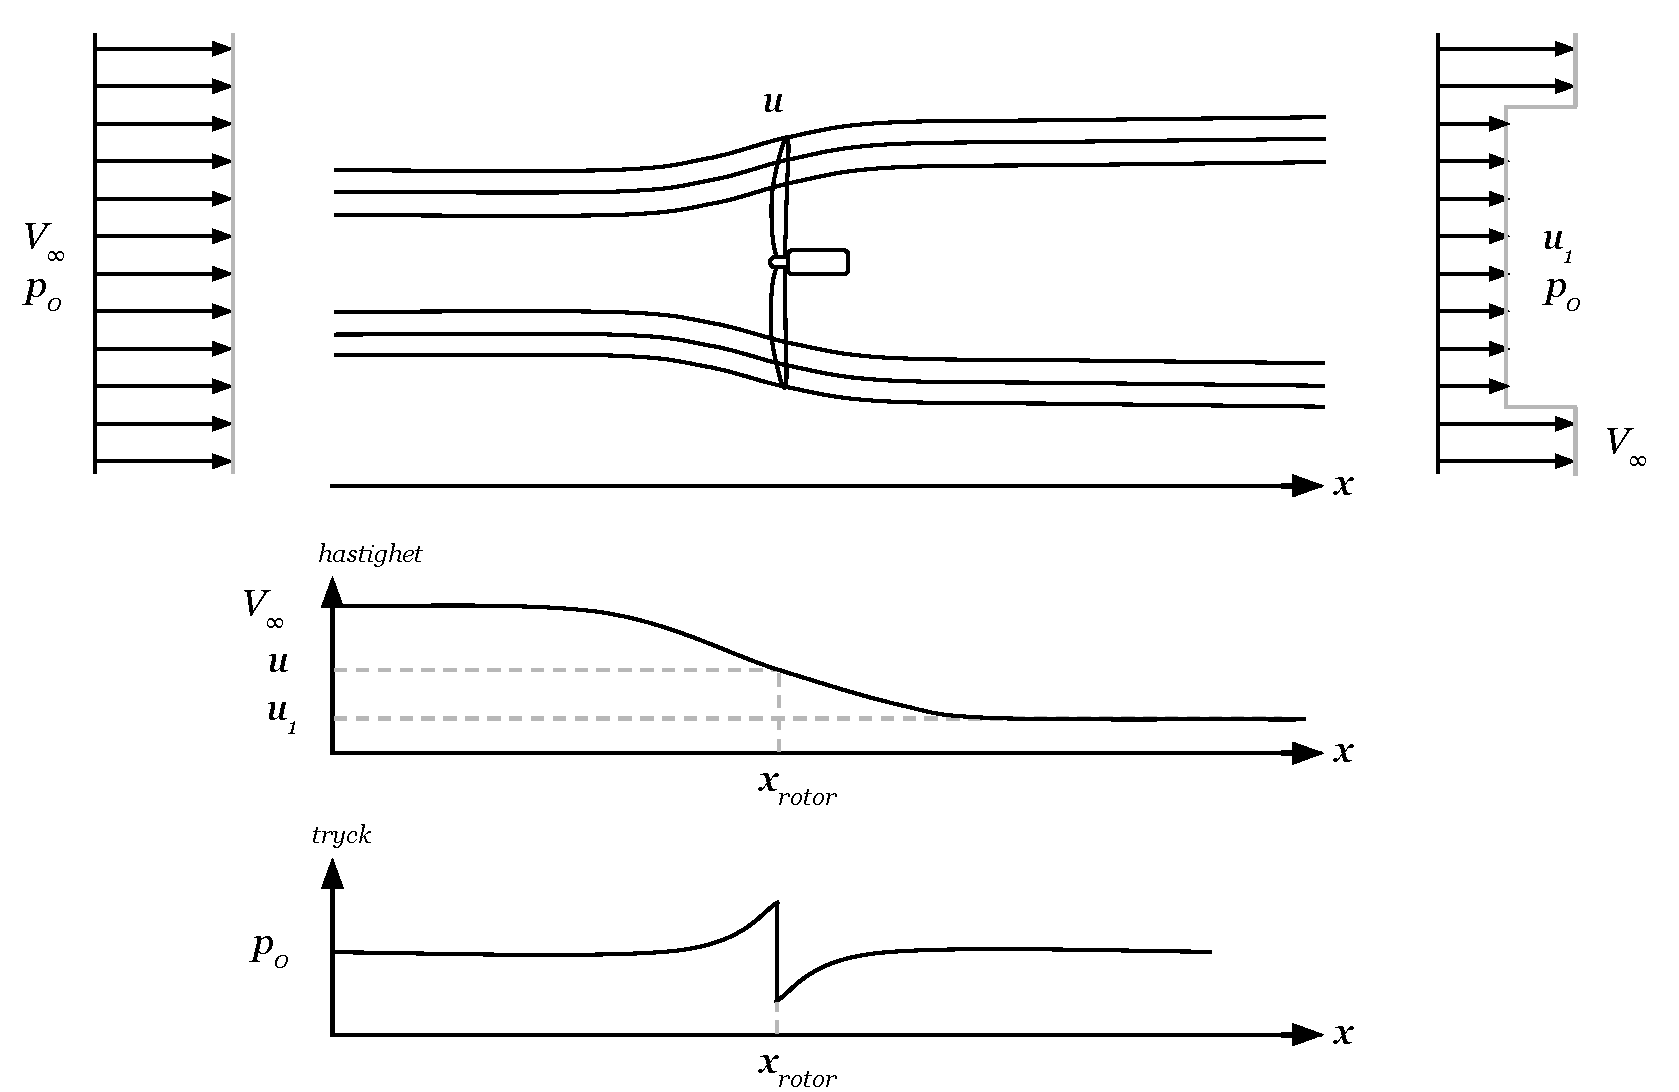
\includegraphics[width=0.9\textwidth]{tryckfall.pdf}
  \caption{Illustration visande strömlinjerna som passerar rotorn samt hur tryck och hastighet förändras över denna. Fritt reproducerat från \citet{hansen}.}
  \label{tryckfall}
\end{figure}

Tryckkraften $T$ ligger i strömningens riktning och är ett resultat av tryckfallet över rotorn.

\begin{equation}\label{thrust} T = \Delta p \pi R^2 \end{equation}

Bernoullis ekvation är nu giltig mellan platsen långt uppströms till precis innan rotorn,

\begin{equation}\label{fore}
p_0 + \frac{1}{2}\rho V_{\infty}^2 = p + \frac{1}{2}\rho u^2
\end{equation}

samt även mellan platsen precis bakom rotorn till långt nedströms,

\begin{equation}\label{efter}
p - \Delta p + \frac{1}{2}\rho u^2 = p_0 + \frac{1}{2} \rho u_1^2
\end{equation}

Kombineras dessa ekvationer erhålls

\begin{equation}\label{pdrop}
\Delta p = \frac{1}{2}\rho (V_{\infty}^2 - u_1^2)
\end{equation}

\begin{figure}[!htb]
  \centering
  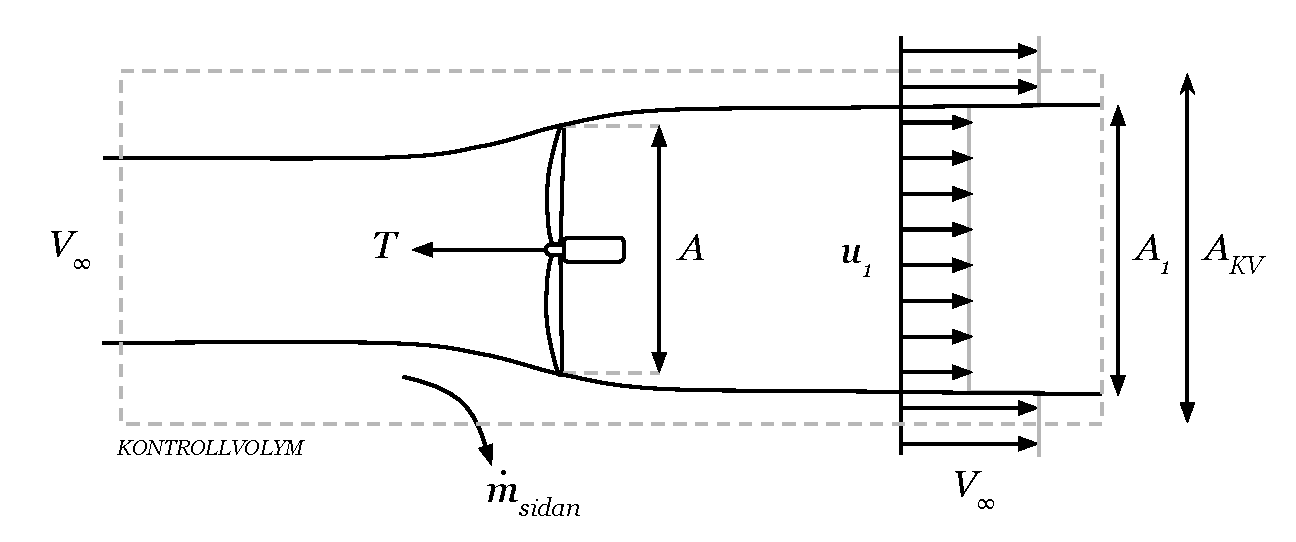
\includegraphics[width=0.9\textwidth]{kontrollvolym.pdf}
  \caption{Kontrollvolym kring den ideala rotorn. Fritt reproducerat från \citet{hansen}.}
  \label{kontrollvolym}
\end{figure}

Ur en analys av en cirkulär kontrollvolym som visas i \fref{kontrollvolym} där stationärt flöde antas, atmosfärstrycket $p_o$ råder nedströms i vaken och att ingen radiell komponent av kraften uppstår kan följande visas

\begin{equation}\label{ekvkontrollvolym}
\rho u_1^2 A_1 + \rho V_{\infty}^2(A_{KV} - A_1) + \dot{m}_{sidan} V_{\infty} - \rho V_{\infty}^2 A_{KV} = -T
\end{equation}

Genom masskonservering kan $\dot{m}_{sidan}$ och totala massflödet $\dot{m}$ erhållas 

\begin{equations}
\begin{align}
        \label{msidan}\dot{m}_{sidan} &= \rho A_1 (V_{\infty} - u_1)\\
        \label{mprick}\dot{m} &= \rho u A = \rho u_1 A_1
\end{align}
\end{equations}

Genom att kombinera ekvationerna \ref{ekvkontrollvolym}, \ref{msidan} och \ref{mprick} fås

\begin{equation}\label{trusty}
T = \rho u A (V_{\infty} - u_1)
\end{equation}

Om $T$ nu ersätts med tryckfallet i ekvation \ref{thrust} fås

\begin{equation}\label{umedel}
u = \frac{1}{2} (V_{\infty} + u_1)
\end{equation}

Vilket visar att hastigheten i rotorplanet är ett medelvärde av friströmshastigheten och vakhastigheten.

\begin{figure}[!htb]
  \centering
  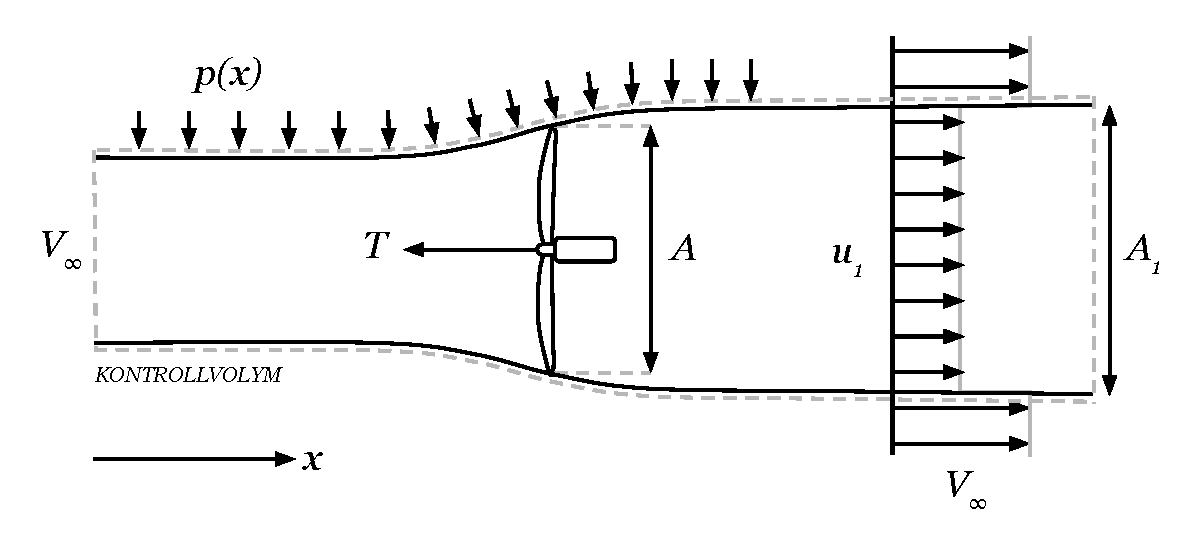
\includegraphics[width=0.9\textwidth]{kontrollvolym2.pdf}
  \caption{Ny kontrollvolym kring den ideala rotorn. Fritt reproducerat från \citet{hansen}. }
  \label{kontrollvolym2}
\end{figure}

Med kontrollvolymen i \fref{kontrollvolym2} och antagandet om ett friktionslöst flöde som inte har någon ändring i intern energi kan det nu visas att effekten i vindkraftverkets axel måste vara 

\begin{equation*}
P =  \underbrace{\rho u A}_{\dot{m}} \left(\frac{1}{2} V^2_{\infty} + \frac{p_0}{\rho} - \frac{1}{2} u^2_1 - \frac{p_0}{\rho}\right)
\end{equation*}

vilket ger

\begin{equation}\label{powwa}
P =  \frac{1}{2}\rho u A (V^2_{\infty} - u_1^2)
\end{equation}

Den axiella induktionsfaktorn $a$ kan nu introduceras som

\begin{equation}
a = \frac{V_{\infty} - u}{V_{\infty}}
\end{equation}

Genom att kombinera den med ekvation \ref{umedel} fås

\begin{equation}\label{adef}
a = \frac{V_{\infty} - u_1}{2 V_{\infty}}
\end{equation}

Detta kan nu introduceras i ekvation \ref{powwa} och \ref{trusty} och resulterar i

\begin{equation}\label{powermeda}
P = 2 \rho V^3_{\infty} a (1 - a)^2 A
\end{equation}

\begin{equation}
T = 2 \rho V^2_{\infty} a (1 - a) A
\end{equation}

$C_P$ är sedan tidigare definierat till 

\begin{equation}
C_P = \frac{P}{\frac{1}{2} \rho V^3_{\infty} A}
\end{equation}

Tillsammans med ekvation \ref{powermeda} och deriverat med avseende på $a$ samt satt lika med noll fås 

\begin{equation}
\frac{\operatorname{d}\!C_P}{\operatorname{d}\!a} = 4(1 - a)(1 - 3a) = 0
\end{equation}

Ur detta kan man se att $C_{P_{max}}$ uppstår när $a = 1/3$ varpå ett $C_P = 16/27 \approx 0.593$. Detta är känt under namnet Betz-gränsen vilket är ett teoretiskt maximum för hur mycket av vindens inneliggande energi som går att ta ut.

På samma sätt som $C_P$ introducerats definieras tryckkraftskoefficienten $C_T$

\begin{equation}
\label{CT}C_T = \frac{T}{\frac{1}{2} \rho V^2_{\infty} A}
\end{equation}

\begin{figure}[!htb]
  \centering
  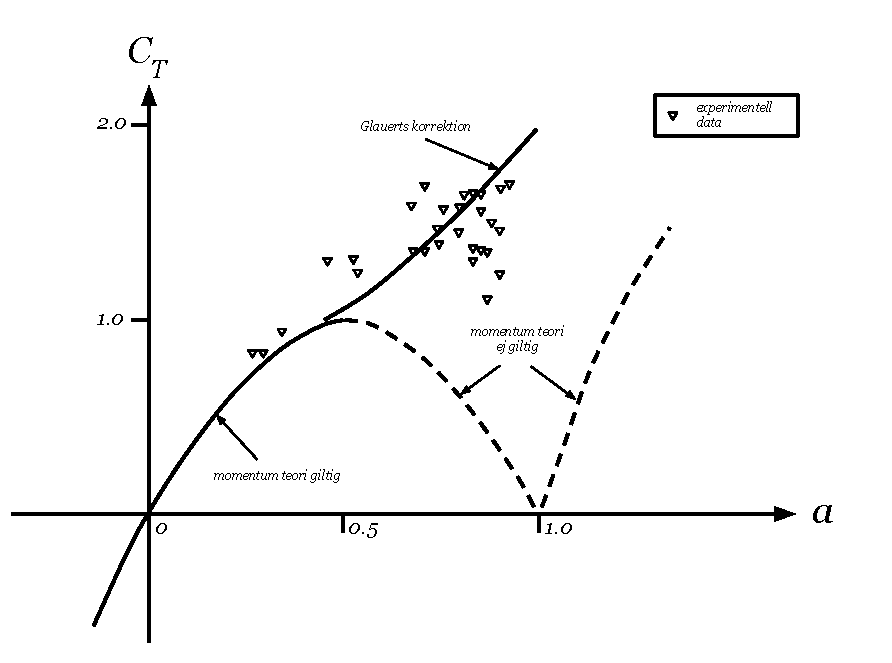
\includegraphics[width=0.8\textwidth]{CT.pdf}
  \caption{Figur visande hur $C_T$ varierar med $a$. Fritt reproducerat från \citet{hansen}. }
  \label{CT}
\end{figure}

Antagandena som fram tills nu gjorts har med experimentella data visats endast giltiga för $a < 0.4$ vilket syns i \fref{CT}. Om rörelsemängsdteorin var giltig över 0.4 hade detta betytt att hastigheten i vaken var negativ vilket inte är fallet. Detta kommer senare att tas hänsyn till.

\begin{figure}[!htb]
  \centering
  \subfigure[Virveln ett flygplan inducerar. Foto: NASA public domain]{
    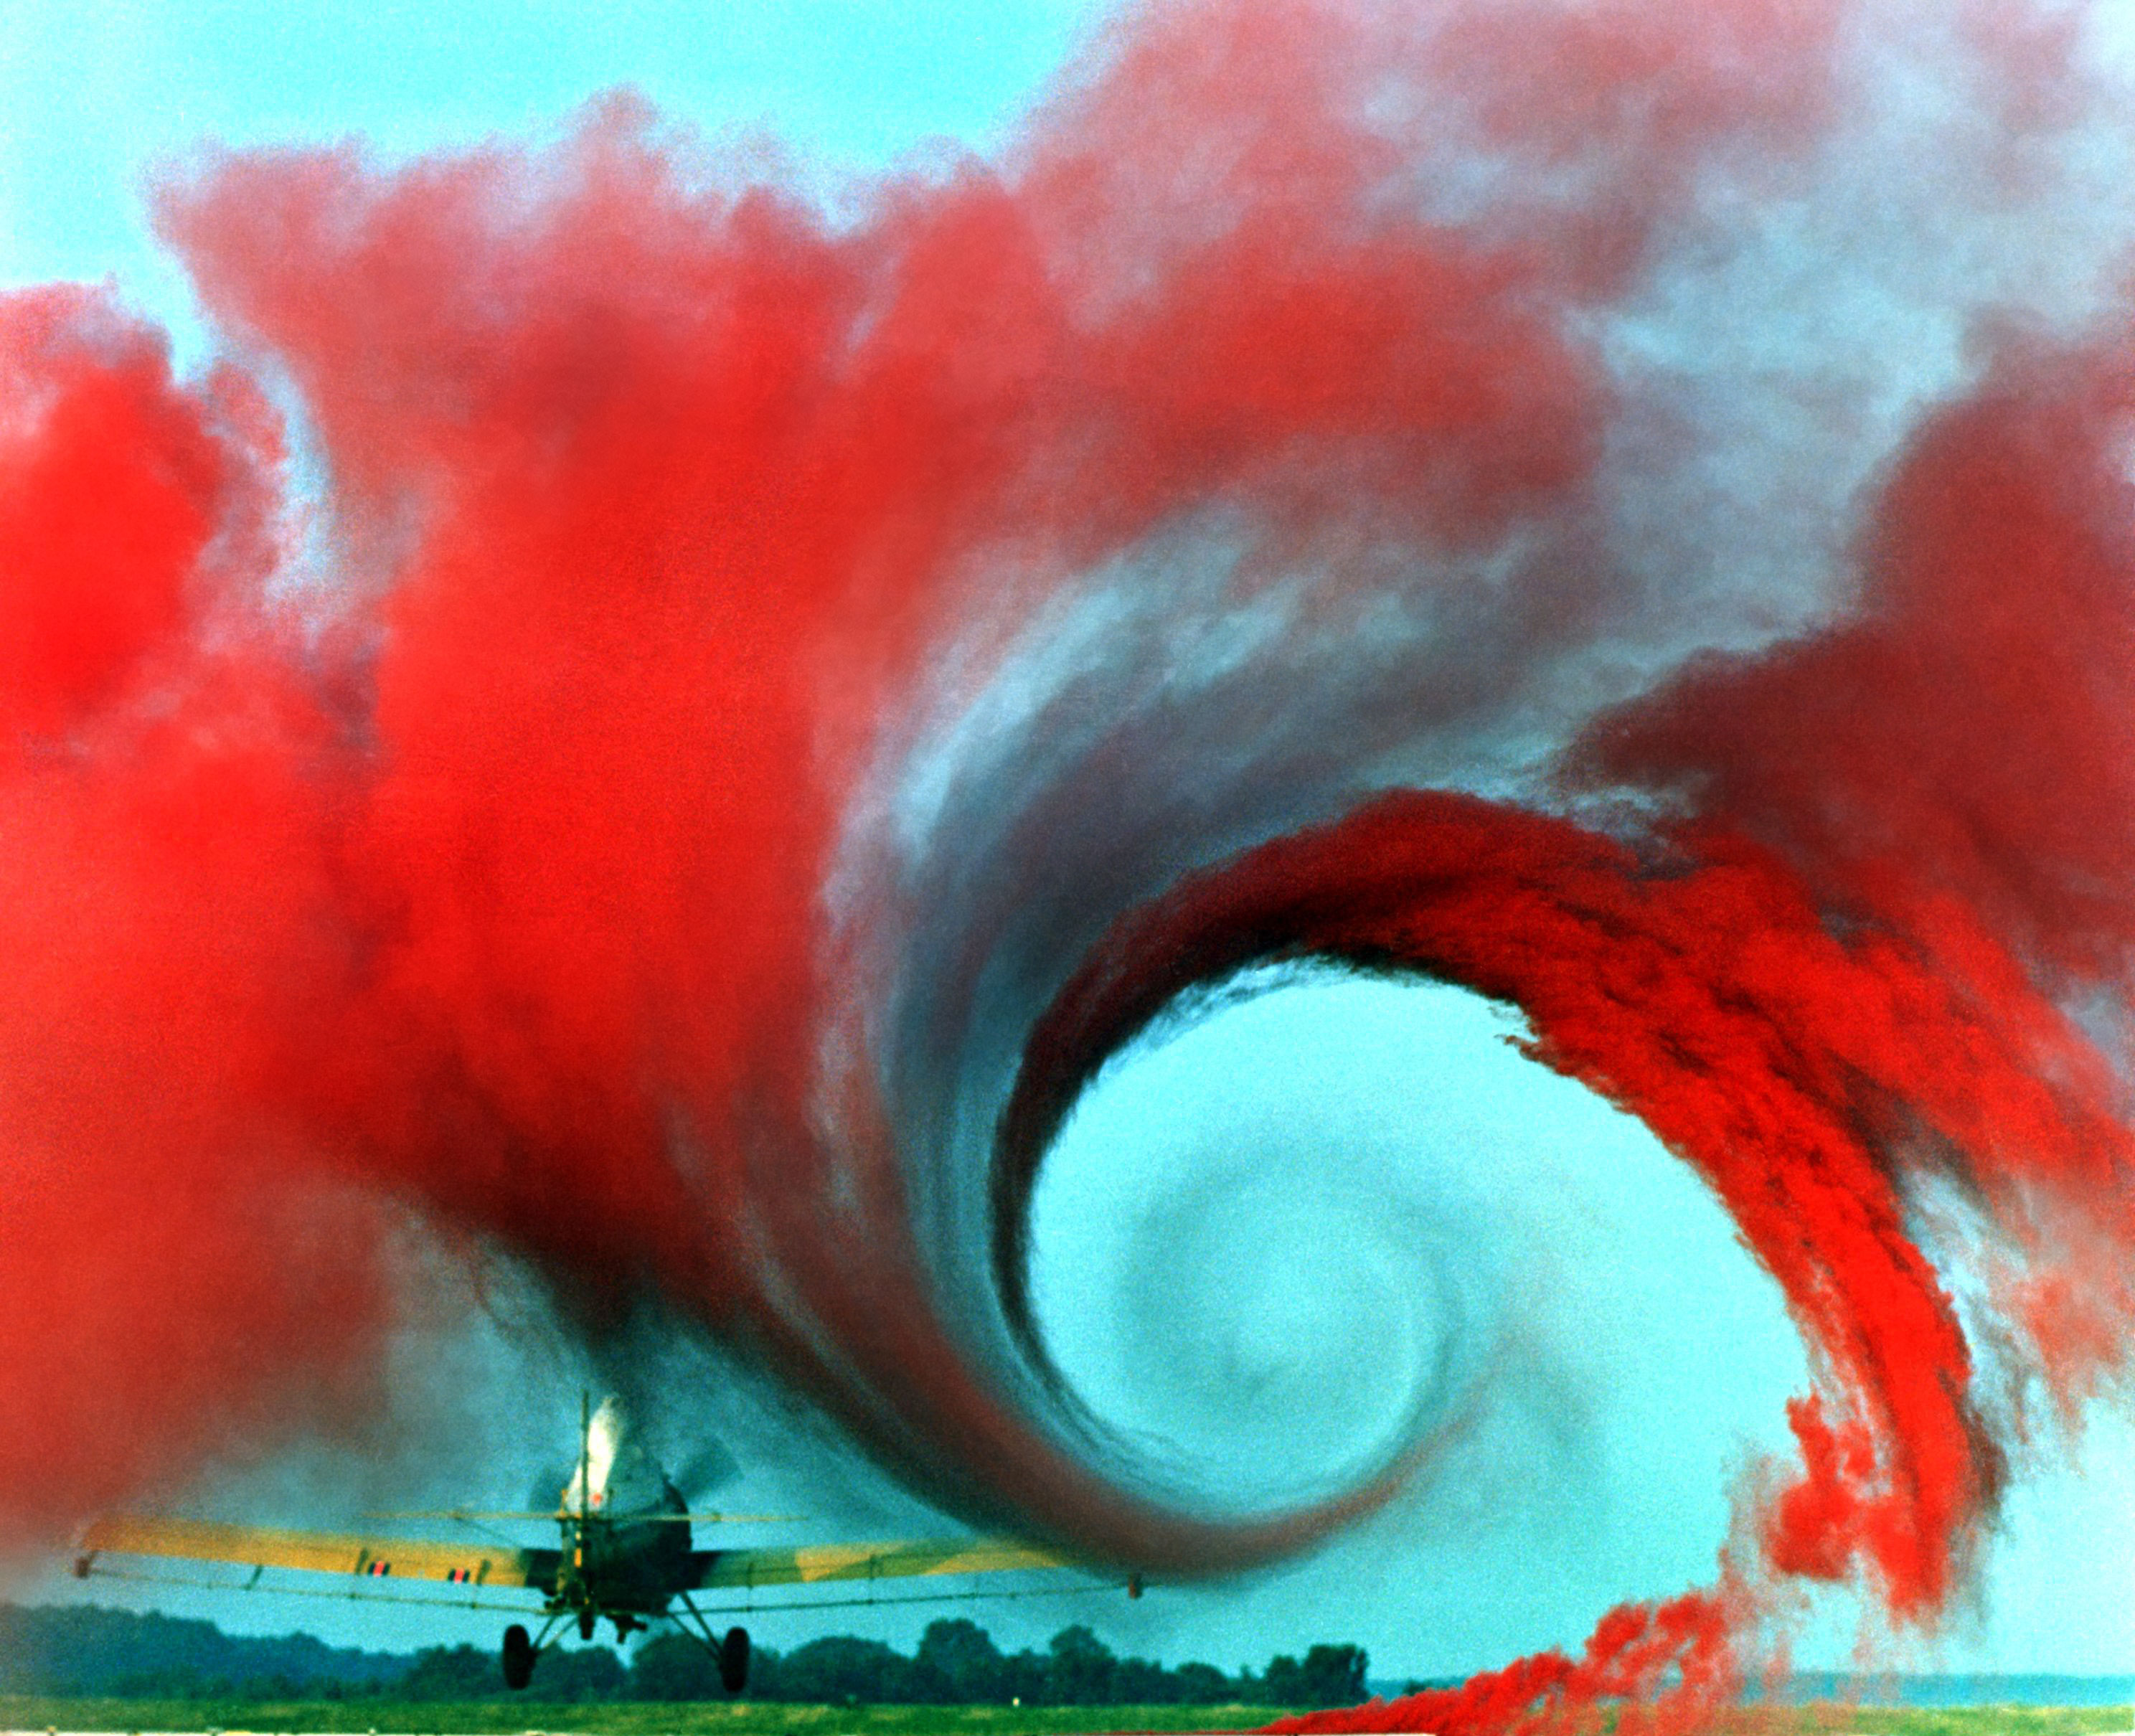
\includegraphics[height=4.2cm]{vortex}
    \label{vortex}
  }
  \subfigure[Virvlarna ett vindkraftverks rotorblad inducerar. Fritt reproducerat från \citet{hansen}]{
    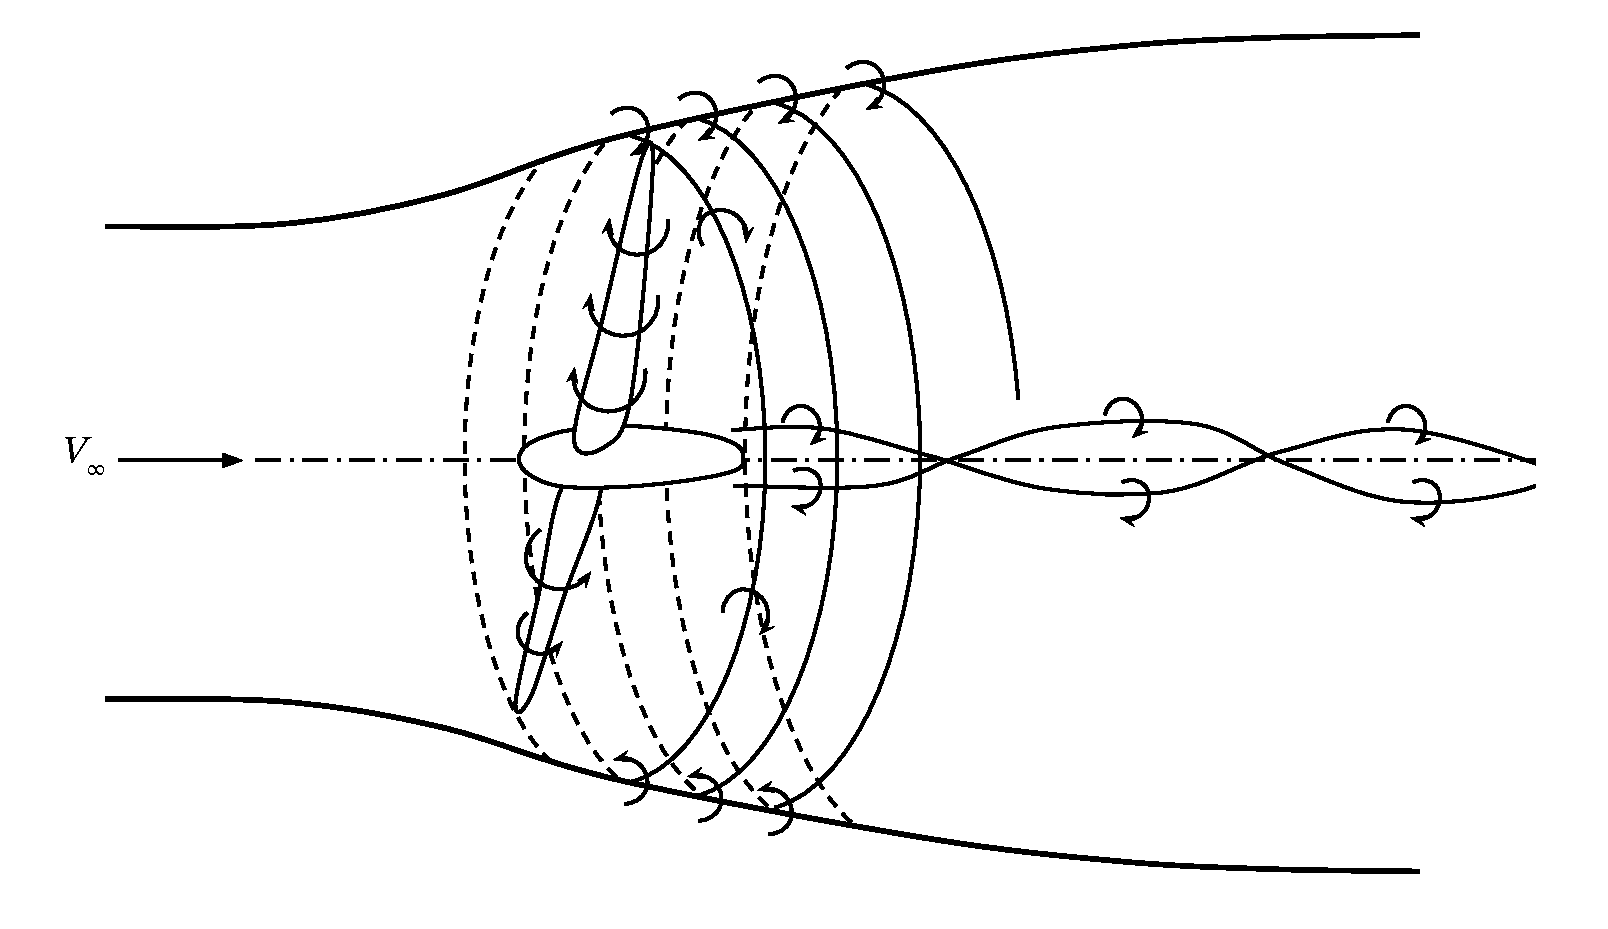
\includegraphics[height=4.2cm]{virvlarfig.pdf}
    \label{virvlarfig}
  }
  \caption{Olika typer av virvlar.}
  \label{virvlar}
\end{figure}

$a$ som tidigare introducerades ska nu visa sig ha en fysikalisk betydelse som framöver är av stor vikt. I \fref{vortex} syns virveln som ett flygplans vinge inducerar. På samma sätt skapar ett vindkraftverks rotorblad virvlar som måste tas hänsyn till. I \fref{virvlarfig} illustreras dessa virvlar.

Systemet av virvlar inducerar en axiell hastighetskomponent i motsatt riktning som den inkommande vinden samt en tangentiell komponent i motsatt riktning till rotationen av rotorbladen. Den axiella hastigheten specificeras med den tidigare nämnda axiella induktionsfaktorn $a$ som $a V_{\infty}$. Den tangentiella hastigheten som uppstår i rotorns vak specificeras med den tangentiella induktionsfaktorn $a'$ som $2 a' \Omega r$.

$2 a' \Omega r$ kallas vidare $C_{\theta}$.

\begin{figure}[!htb]
  \centering
  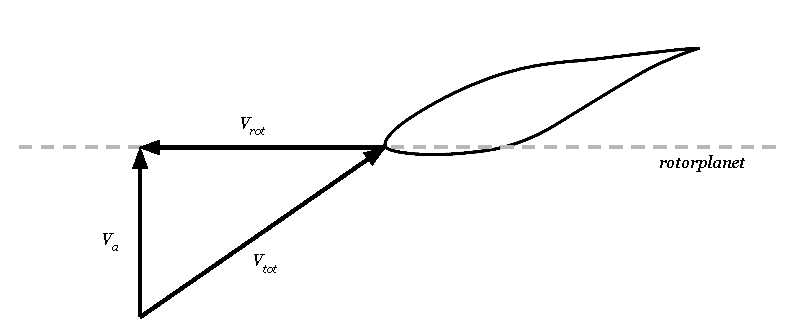
\includegraphics[width=0.7\textwidth]{indushast.pdf}
  \caption{Hastighetskomponenterna som en vingprofil upplever. Fritt reproducerat från \citet{hansen}.}
  \label{indushast}
\end{figure}

Vingprofilerna i rotorbladet påverkas därför av hur dessa nya hastihetskomponenter beter sig. I \fref{indushast} syns dessa och följande samband gäller

\begin{equations}
\begin{align}
    V_a &= (1 - a)V_{\infty}\\
    V_{rot} &= (1 + a')\Omega r
\end{align}
\end{equations}

\subsubsection{``Blade element momentum''-metoden}

``Blade element momentum''-metoden kopplar samman den endimensionella rörelse-\\mängdsteorin med det som faktiskt händer lokalt längs bladet. Den kontrollvolymen som i endimensionella rörelsemängdsteorin introducerade delas nu upp i ett antal element med samma höjd $\operatorname{d}\!r$ där $r$ är den lokala radien och $R$ rotorns fulla radie. Detta ses i \fref{streamtubedr}. Dessa avgränsas av flödeslinjer vilket alltså betyder att inget flöde kan ske mellan dessa element vilket är ett antagande \textsc{Bem}-teorin vilar på.

\begin{figure}[!htb]
  \centering
  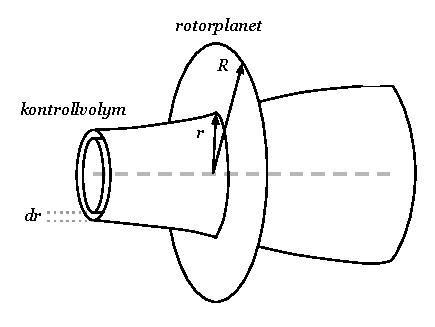
\includegraphics[width=0.7\textwidth]{streamtubedr.pdf}
  \caption{Kontrollvolym med formen som ett rör genom rotorplanet. Fritt reproducerat från \citet{hansen}.}
  \label{streamtubedr}
\end{figure}

Rörelsemängdsekvationen på integralform kan nu appliceras på ett element och ge tillskottet av tryckkraft i det elementet

\begin{equation}
\operatorname{d}\!T = (V_{\infty} - u_1)\operatorname{d}\!\dot{m} = 2 \pi r \rho u (V_{\infty} - u_1)\operatorname{d}\!r
\end{equation}

Vridmomentet $\operatorname{d}\!Q$ kan på samma sätt tas fram om rotationens hastighet i friströmmen sätts till noll och den i vaken sätts till $C_{\theta}$

\begin{equation}
\operatorname{d}\!Q = r C_{\theta} \operatorname{d}\!m = 2 \pi r^2 \rho u C_{\theta} \operatorname{d}\!r
\end{equation}

Genom att nu föra in det som tagits fram gällande $a$ i ekvation \ref{adef} samt $C_{\theta} = 2 a' \Omega r$ kan tryckkraft och vridmoment skrivas om till

\begin{equations}
\begin{align}
\label{firstdT}\operatorname{d}\!T &= 4 \pi r \rho V_{\infty}^2 a (1 - a) \operatorname{d}\!r \\
\label{firstdQ}\operatorname{d}\!Q &= 4 \pi r^3 \rho V_{\infty} \Omega (1 - a) a' \operatorname{d}\!r 
\end{align}
\end{equations}

\begin{figure}[!htb]
  \centering
  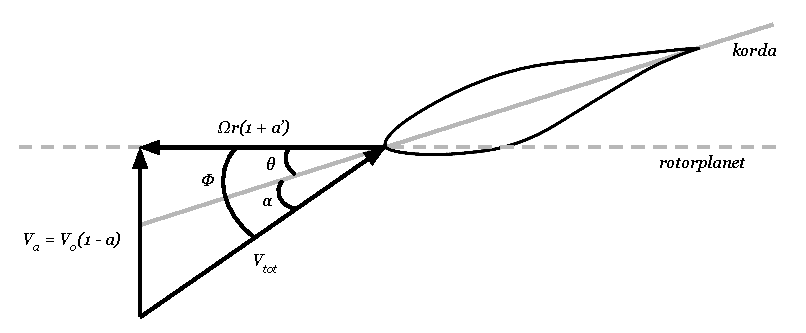
\includegraphics[width=0.9\textwidth]{vrotva.pdf}
  \caption{Hastighetskomponenterna en vingprofil i rotorplanet upplever. Fritt reproducerat från \citet{hansen}.}
  \label{vrotva}
\end{figure}

Om nu $V_{rot}$ och $V_a$ placeras ut som i \fref{vrotva} kan ses att vingprofilen i själva verket utsätts för hastigheten $V_{tot}$. \emph{Pitch} i varje lokal vingprofil längs rotorbladet är en kombination av bladets \emph{pitch} ($\theta_p$) och \emph{twist} ($\beta$) som $\theta = \theta_p + \beta$. $\phi$ är den totala vinkeln mellan rotorplanet och hastigheten $V_{tot}$.

Vingprofilens lokala angreppsvinkel ($\alpha$) blir alltså

\begin{equation*}
\alpha = \phi - \theta
\end{equation*}

\fref{vrotva} ger även att 

\begin{equation*}
\phi = \arctan \frac{(1 - a)V_{\infty}}{(1 + a')\Omega r}
\end{equation*}

Lyft- och motståndskraften har tidigare visas implicit i \ref{c_l}. Lyftkraften ligger vinkelrätt mot den inkommande vindhastigheten $V_{tot}$ och motståndskraften i samma riktning. Därför gäller

\begin{equations}
\begin{align}
    l = \frac{1}{2} \rho V_{tot}^2 c C_l \\
    d = \frac{1}{2} \rho V_{tot}^2 c C_d
\end{align}
\end{equations}

Där små bokstäver för lyft- och motståndskraft används för att påpeka att det är tvådimensionella krafter.

\begin{figure}[!htb]
  \centering
  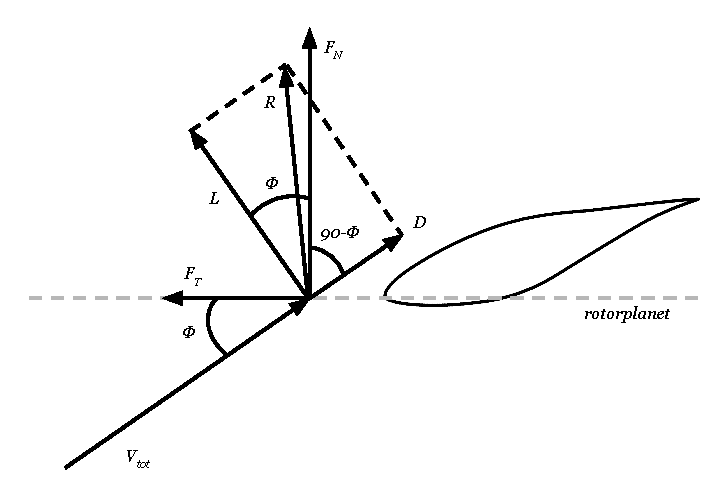
\includegraphics[width=0.8\textwidth]{liftdragproj.pdf}
  \caption{Krafter upplevda av en vingprofil i rotorplanet. Fritt reproducerat från \citet{hansen}.}
  \label{liftdragproj}
\end{figure}

Eftersom endast normal- och tangentialkraften i rotorplanet är av intresse projiceras krafterna till $F_n$ och $F_t$ vilket syns i \fref{liftdragproj} enligt

\begin{equations}
\begin{align}
    F_n &= l \cos \phi + d \sin \phi  \\
    F_t &= l \sin \phi - d \cos \phi
\end{align}
\end{equations}

Dessa kan nu göras dimensionslösa genom att delas på $\frac{1}{2} \rho V_{tot}^2 c$ och blir då

\begin{equations}
\begin{align}
\label{Cn} C_n &= C_l \cos \phi + C_d \sin \phi  \\
\label{Ct} C_t &= C_l \sin \phi - C_d \cos \phi
\end{align}
\end{equations}

där 

\begin{equations}
\begin{align}
\label{Cn2} C_n &= \frac{F_n}{\frac{1}{2}\rho V_{tot}^2 c}\\
\label{Ct2} C_t &= \frac{F_t}{\frac{1}{2}\rho V_{tot}^2 c}
\end{align}
\end{equations}

Ur geometrin i \fref{vrotva} kan även ses att 

\begin{equations}
\begin{align}
\label{vtotsin} V_{tot} \sin \phi &= V_{\infty} (1 - a) \\
\label{vtotcos}V_{tot} \cos \phi &= \Omega r (1 + a')
\end{align}
\end{equations}

Lokal \emph{solidity} $\sigma$ införs som andelen yta som täcks med blad i en radiell position

\begin{equation}
\label{solidity}\sigma (r) = \frac{c(r)B}{2 \pi r}
\end{equation}

Notera att detta är lokalt vid varje position på rotorbladet och därför en funktion av radien. $B$ är antalet blad på vindkraftverket, $c(r)$ den lokala kordan och $r$ den radiella positionen.

Krafterna $F_n$ och $F_t$ multipliceras eftersom de är tvådimensionella med sitt radiella element $\operatorname{d}\!r$ och ger tillskottet av \emph{trust} $\operatorname{d}\!T$ och vridmoment $\operatorname{d}\!Q$

\begin{equations}
\begin{align}
    \operatorname{d}\!T &= B F_n \operatorname{d}\!r \\
\label{dQen}\operatorname{d}\!Q &= r B F_t \operatorname{d}\!r
\end{align}
\end{equations}

Använder ekvation \ref{Cn2} för att ersätta $F_n$ och ekvation \ref{vtotsin} för $V_{tot}$ fås istället

\begin{equation}
\label{dTkrongling}\operatorname{d}\!T = \frac{1}{2}\rho B \frac{V_{\infty}^2(1 - a)^2}{\sin^2 \phi} c C_n \operatorname{d}\!r
\end{equation}

Används på liknande sätt ekvation \ref{Ct2} för att ersätta $F_t$ och ekvation \ref{vtotsin} och \ref{vtotcos} blir nu istället \ref{dQen}

\begin{equation}
\label{dQkrongling}\operatorname{d}\!Q = \frac{1}{2}\rho B \frac{V_{\infty} (1 - a) \Omega r (1 + a')}{\sin \phi \cos \phi} c C_t r \operatorname{d}\!r
\end{equation}

Likställs $dT$ för \ref{firstdT} och \ref{dTkrongling} samt appliceras $\sigma$ (\ref{solidity}) kan ett utryck för $a$ nu härledas

\begin{equation}
\label{finala} a = \frac{1}{\frac{4 \sin^2 \phi}{\sigma C_n} + 1}
\end{equation}

Om \ref{firstdQ} och \ref{dQkrongling} likställs fås på samma sätt 

\begin{equation}
\label{finala} a' = \frac{1}{\frac{4 \sin \phi \cos \phi}{\sigma C_t} - 1}
\end{equation}

\subsubsection{Prantl topp-förluster}

Tidigare i \ref{1dmomentumteori} har antaganden gjorts att vindkraftverkets rotor bestått av ett oändligt antal rotorblad. När ett begränsat antal rotorblad som t.ex. 3 st används påverkar detta virvlarna som uppstår i vaken. För att kompensera för detta används ofta Prandtls korrektionsfaktor $F$. För en fullständig härledning hänvisas läsaren till \citet{glauert}.

\begin{equation}
\label{F} f = \frac{B}{2} \frac{R-r}{r \sin \phi}
\end{equation}

Sätts in i

\begin{equation}
\label{F} F = \frac{2}{\pi} \arccos (e^{-f}) 
\end{equation}

Om ekvation \ref{firstdT} och \ref{firstdQ} multipliceras med $F$ och $a$ och $a'$ löses ut fås istället

\begin{equations}
\begin{align}
   \label{aFkorrad} a &= \frac{1}{\frac{4 F \sin^2 \phi}{\sigma C_n} + 1} \\
   \label{aprimkorrad} a' &= \frac{1}{\frac{4 F \sin \phi \cos \phi}{\sigma C_t} - 1}
\end{align}
\end{equations}

\subsubsection{Glauert-korrektion}

I \fref{CT} visades att för $a > 0.4$ behövs en empirisk korrektion göras för $C_T$. Detta görs enligt förfarandet föreslagit i \citet{buhl} eftersom annars en numerisk instabilitet kan uppstå \citep{adyntheory}.

När $C_T > 0.96F$ vilket är samma som $a > 0.4$ gäller därför 

\begin{equation}
\label{aKorr} a = \frac{18F-20-3\sqrt{C_T(50-36F) + 12F(3F-4)}}{36F-50}
\end{equation}

$C_T$ tas nu istället fram genom att sätta samman dess definition \ref{CT} för ett radiellt element 

\begin{equation}
C_T = \frac{\operatorname{d}\!T}{ \rho V^2_{\infty} \pi \operatorname{d}\!r}
\end{equation}

med \ref{dTkrongling} vilket ger

\begin{equation}
\label{CTNY}C_T = \frac{(1 - a)^2\sigma C_n}{\sin^2 \phi}
\end{equation}


\pagebreak
\subsubsection{Implementering av \textsc{Bem}-algoritmen}

Alla ekvationer som behövs har nu presenterats och $a$ och $a'$ kan nu iterativt tas fram för varje radiellt element på rotorn. Detta görs förslagsvis enligt följande steg:

\begin{enumerate}
  \item Initialt sätts $a = 0$ och $a' = 0$
  \item Vinkeln $\phi = \arctan \frac{(1 - a)V_{\infty}}{(1 + a')\Omega r}$ beräknas så att $\alpha = \phi - \theta$ kan tas fram.
  \item $C_l$ och $C_d$ interpoleras fram från datan som i denna studie kommer från \textsc{Xfoil}. 
  \item $C_n$ och $C_t$ beräknas enligt ekvationerna \ref{Cn} och \ref{Ct}.
  \item Räkna ut Prantl topp-förlust-faktorn $F$ genom ekvation \ref{F} samt $C_T$ med ekvation \ref{CTNY}
  \item Beroende på värde på $C_T$ beräkna $a$ med ekvation \ref{aKorr} eller \ref{aFkorrad}.
  \item Räkna ut $a'$ med ekvation \ref{aprimkorrad}
  \item Jämför värdet på $a$ med det tidigare. Skiljer de sig mindre åt än tolleransnivån har konvergens nåtts. Om inte, gå tillbaka till steg 2.
  \end{enumerate}
  
När $a$ och $a'$ erhållits för alla radiella element längs rotorn kan nu även vridmomentet för alla radiella element beräknas med exempelvis ekvation \ref{dQkrongling}.

Genom att sedan integrera dessa tillskott $\operatorname{d}\!Q$ till vridmomentet, och med antagandet att allt före $r_{hub}$ endast genererar motståndskraft - fås det totala vridmomentet i rotorn. 

\begin{equation}
Q = \int_{r_{hub}}^R \operatorname{d}\!Q
\end{equation}

Detta används tillsammans med vinkelhastigheten ($\Omega$) för att få fram rotorns effekt

\begin{equation}
P = Q \Omega
\end{equation}

För mer utförlig beskrivning av ekvationer som här presenterats hänvisas läsaren till \citet{wehb}.
  


\subsection{Optimeringslära}

Studiens mål och senare metodologi  baseras att ett optimeringsproblem där så mycket effekt som möjligt ska tas ut ur vinden. Därför presenteras här optimeringsterminologi och optimeringsalgoritmer som senare används.

\begin{figure}[!htb]
  \centering
  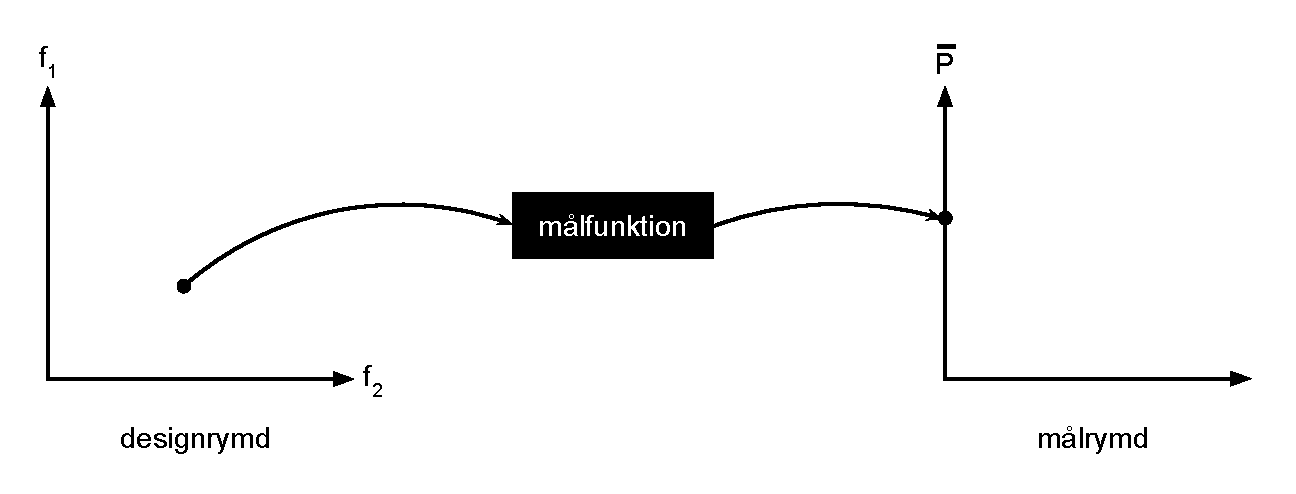
\includegraphics[width=0.9\textwidth]{designmalrymd}
  \caption{Illustration visande hur designrymden utvärderas av målfunktionen för att ge en målrymd.}
  \label{designmalrymd}
\end{figure}

Ett optimeringsproblem definieras av sina designvariabler, designrymd, dess målfunktion och målrymd (se \fref{designmalrymd}). Designvariablerna utgör de variabler som kan varieras för för att få olika resultat. Givet $N$ antal designvariabler $\left\{f_1, f_2, \dots, f_N\right\}$ (i \fref{designmalrymd} är $N=2$) definieras designrymden varpå målfunktionen utvärderar dessa för att returnera en målrymd. I denna studien är målrymden endast ett reellt tal eftersom optimeringen av vindkraftverkets rotorblad endast görs med avseende på dess genomsnittliga effekt $\overline{P}$. Eftersom målfunktionen maximeras kallas ibland även målfunktionen för \emph{fitness-funktion}.

\subsubsection{Andra författares val av målfunktion}

Valet av ett optimeringsproblems målfunktion är av yttersta vikt för vilket resultat som kommer fås. \citet{Dansken, LowRe, Grasso} optimerar endast en vingprofils lyft- och motståndskoefficienter ($C_l$ och $C_d$) över rimliga angreppsvinklar. \citet{Cencelli} gör optimeringen på vindkraftverkets effektkoefficient ($C_P$) vid ett par olika vindhastigheter. 

Andra författare tar ett större grepp och väljer att maximera ett vindkraftverks årliga produktion. \citet{Victoria} låter ett vindhastighetshistogram vara styrande. Detta är ett intressant förhållningssätt eftersom vindkraftverkets riktiga produktion för en specifik plats då nås. Effektkurvan matchas då med vindhastighetshistogrammet som beskriver andelen av tid som en viss vindhastighet förekommer varpå genomsnittseffekten $\overline{P}$ kan tas fram.

\subsubsection{Optimeringsalgoritmer}
Lämpliga optimeringsmetoder som studerats har antingen använt sig av gradient för optimeringen eller inte. I \citet{Victoria} används gradientmetoden SQP (sequential quadratic programming). Fördelen är att konvergens snabbare kan uppnås med en gradient som visar i vilken riktning optimeringen bör fortskrida, men har den stora nackdelen att lokala max/min ofta står för konvergensen. 

Därför är genetiska algoritmer väldigt återkommande i den studerade litteraturen då de är en metod som når globala max/min \citep{Benini, 5MWkillen, LowRe, CST, Dansken}. Flera varianter på genetiska algoritmer finns. ECGA är en variant på genetisk algoritm som utlovar snabbare konvergens med mindre populationsstorlekar \citep{Xiong}. \citet{Grasso} utlovar samma sak med det som kallas microGA.

``Particle swarm''-metoden är även den en gradientlös metod som imiterar ett flockdjurs tendens att efterlikna andra individers framgångsrika beteende. I \citet{Cencelli} används metoden framgångsrikt.  



\subsubsection{Genetiska algoritmer}

En genetisk algoritm är en optimering som hämtar terminologi och inspiration från evolutionen som sker i naturen. Principen är att individer med goda egenskaper kommer premieras i evolutionen genom att deras arvsmassa förs vidare i större utsträckning än mindre lyckade individer.

Följande begrepp är centrala och dess betydelse listas här:

\begin{description}
  \item[Individ] En möjlig lösning på optimeringsproblemet. I denna studie kommer varje individ vara ett vindkraftverk.
  \item[Population] En grupp av individer.
  \item[Arvsmassa] En individs bakomliggande genetiska uppsättning som ger upphov till individens egenskaper. I detta fallet är det vindkraftverkets vingprofiler, korda-distribution och \emph{twist}-distribution längs rotorbladet. Detta representeras av en sträng siffror eller bokstäver $G = \left\{ g_1, g_2, \dots, g_n\right\}$.
  \item[\emph{Fitness}-funktion] Målfunktionen som utvärderar individerna. 
\end{description}

En initial population individer inleder den genetiska algoritmen. Hur bra en individ är, avgörs av den så kallade \emph{fitness}-funktionen som i denna studien utgörs av \textsc{Bem}-algoritmen. 

När alla individer har tilldelats ett \emph{fitness}-värde kan individerna ordnade efter \emph{fitness} tilldelas en partner som deras arvsmassa blandas med enligt en förutbestämd sannolikhet. Vid korsningen av arvsmassa sker även vissa mutationer med en bestämd sannolikhet. Efter detta sker \emph{fitness}-utvärderingen på nytt och proceduren upprepas tills ett förutbestämt antal generationer passerat eller att ett \emph{fitness}-mål uppnås.


\section{Relevans för studien}
I litteraturstudien har det framkommit att optimering av ett vindkraftverk ofta görs med målfunktioner som inte representerar produktionen för ett vindkraftverk på ett specifikt vindförhållande. Det är därför rimligt att i optimeringen fortsätta ta hänsyn till vindhastighetsfördelningen vilket utifrån litteraturstudien  endast \citet{Victoria} gör. \citet{Victoria} har en väldigt begränsad designrymd där endast vingprofiler i NACA 44XX-serien används. Detta bjuder in till att ta vid där de slutade och utöka med en större designrymd med fler vingprofiler.

%% Hör inte hemma. Kan jag komma på en annan vinkel för Fritt reproducerat frånp?
\begin{comment}Det stora antalet sätt att representera vingprofiler är en produkt av att tidigare författare försökt hitta representationer med så få parametrar som möjligt utan för den delen inskränka designrymden. Detta 

%% ----

\rework{Python är ett kraftfullt, enkelt programmeringsspråk med högt pedagogiskt värde då koden är lättläst även för den som inte kan Python. Att använda Python som programmeringsspråk är därmed ett medvetet val där det till skillnad från t.ex. \textsc{MatLab} även är helt öppet. En kommersiell licens för \textsc{MatLab} kostar idag 17 500 \citep{MATLAB} vilket begränsar tillgången för de utan medel. Mitt program kommer därför vara helt oförknippat med några kostnader.}

\end{comment}

\section{Avgränsningar}
\textsc{Xfoil} har visat sig vara ett välanvänt alternativ för att ta fram en vingprofils aerodynamiska egenskaper. Eftersom resultaten visats vara goda kommer inga utförliga försök till att verifiera \textsc{Xfoil}s giltighet att göras. Vidare kommer inga andra programvaror att beaktats eftersom litteraturstudien även visat att t.ex. \textsc{cfd} kommer till för stor beräkningskostnad.

I denna studie beaktas uteslutande vindhastighet som oberoende av rumskoordinater och vid stationärt tillstånd då detta är förutsättningar för \textsc{Bem}. 

Luft betraktas i studien som en inkompressibel fluid. Detta trots att vindhastigheter vid vingbladens topp på vindkraftverk av megawatt-klass kan komma så långt som mach 0.25-0.3 \citep{XfoilVerifikation}.

Strukturella aspekter som belastningen i rotorbladets struktur tas med i ett par studier och kan ge betydande påverkan på resultatet \citep{5MWkillen, Victoria}. Detta kommer här anses ligga utanför studiens omfattning för att istället tas hänsyn till med enklare restriktioner.

Mer avancerade genetiska algoritmer har framkommit i litteraturstudien, men en mer djupgående analys av deras skillnader anses ligga utanför denna rapportens ambition.




%% ----------------------------------------------------------------
%% Method.tex
%% ---------------------------------------------------------------- 
\chapter{Metod} \label{Chapter:Metod}

\begin{sidewaysfigure}
  \centering\thisfloatpagestyle{metod}%
  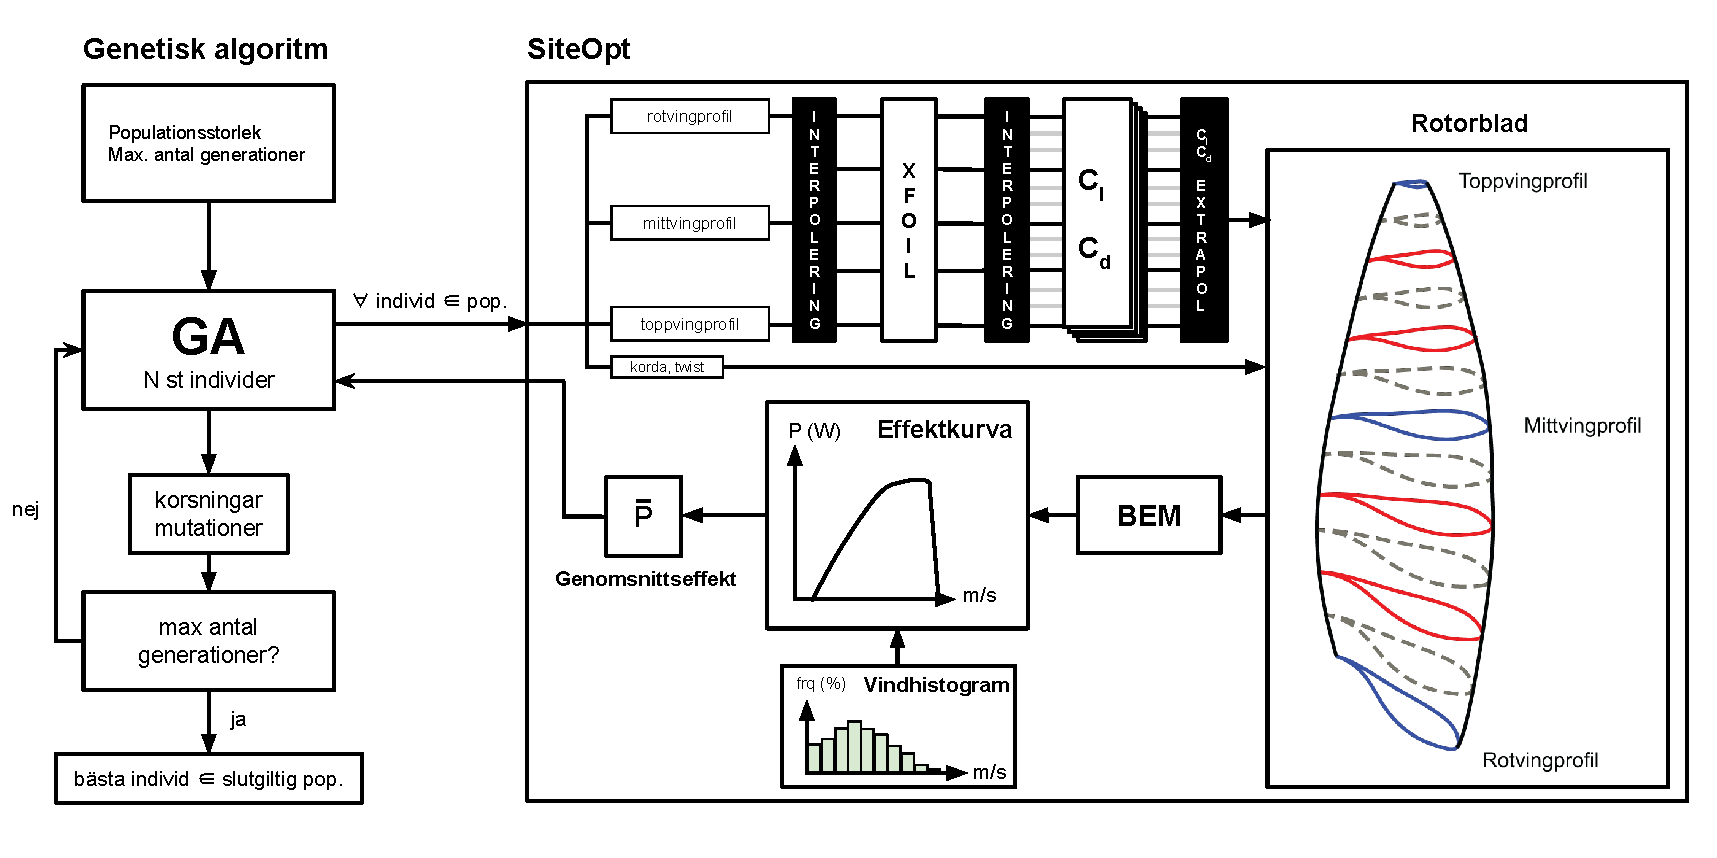
\includegraphics[width=0.8\textwidth]{metod}
  \caption{Överblick av studiens metod}
  \label{metod}
\end{sidewaysfigure}

För studien har en enklare programvara som implementerar \textsc{Bem}-teorin samt sköter kommunikation med \textsc{Xfoil} och optimeringsalgoritmen utvecklats. Denna hänvisas vidare till som SiteOpt och finns i sin helhet i \hyperref[Chapter:kallkod]{Appendix A}. Hur olika delar hänger ihop åskådliggörs även i \fref{metod}.

Sammantaget är SiteOpts funktion att utvärdera varje individ som optimeringsalgoritmen skapar. Detta görs genom att vingprofiler från individens arvsmassa skapas och utvärderas i \textsc{Xfoil}. Mellanliggande vingprofiler längs rotorbladet interpoleras fram och utvärderas även de. 

Individen och dess lyft- och motståndskoefficienter ($C_l$ och $C_d$) för vingprofilerna samt korda- och twist-distributionen kan nu med \textsc{Bem} generera en effektkurva. Med vindhastighetshistogrammet SiteOpts användare specificerat fås en genomsnittseffekt $\overline{P}$ som agerar underlag för optimeringsalgoritmen. Denna styr sedan vilka individer som förs vidare till nästa generation genom korsningar. De nya individerna utsätts även för mutationer.

\pagebreak 

\section{Vingprofilsrepresentation med B-splines}
\label{b-splines}

\begin{figure}[!htb]
  \centering
  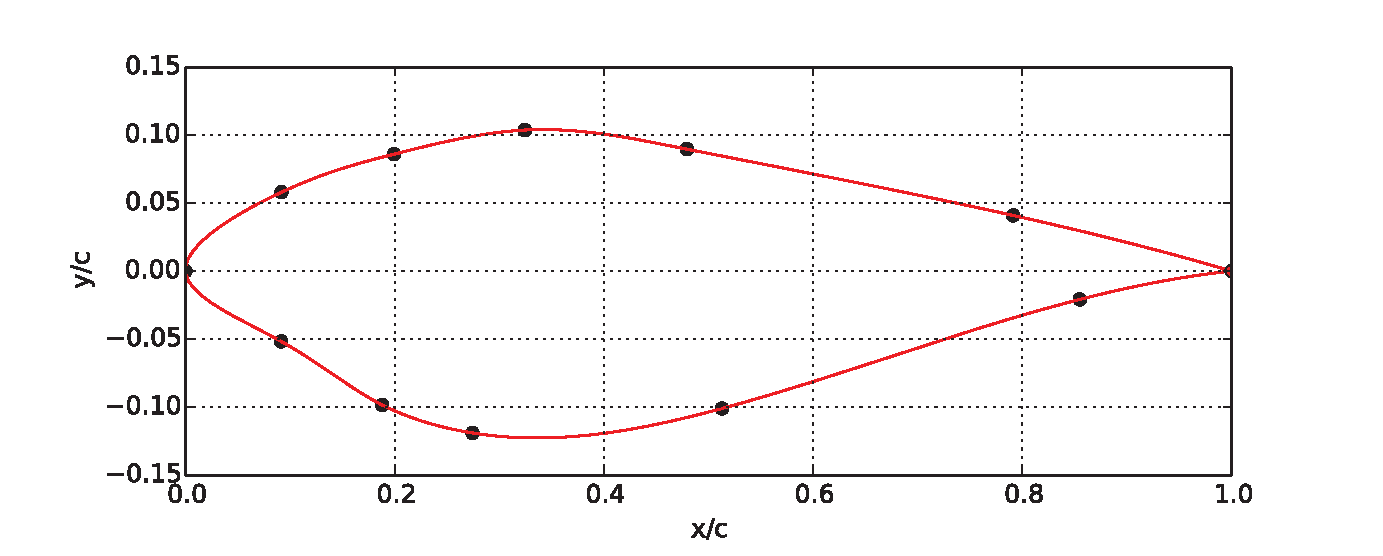
\includegraphics[width=1\textwidth]{connectTheDots3}
  \caption{Vingprofilsrepresentation genom sammanbindning av diskreta punkter genom B-spline-interpolation}
  \label{connectTheDots2}
\end{figure}

I litteraturstudien framkom att för många designvariabler i ett optimeringsproblem leder till höga beräkningskostnader. Av den anledningen ska antalet designvariabler hållas lågt utan att för den delen inskränka för mycket på designrymden. CST-metoden \citep{CST} som använde ett begränsande polynom samt \citet{Cencelli} där istället fem grundprofiler blandades gör båda för stora inskränkningar på designrymden och valdes därför bort.

Kvar blir sammanbindning av diskreta punkter genom Beziér-kurvor eller B-splines, och eftersom B-splines ger en väldigt enkel representation där alla punkter kan genomlöpas valdes denna metod. Detta betydde att existerande vingprofiler enkelt kunde återskapas med B-splines under arbetets gång.

Programmeringsspråket Pythons inbyggda interpoleringsmodul \lstinline[breaklines=true]!splprep! som implementerar en B-spline så som beskrivet av \citet{B-spline} användes med parametern \lstinline[breaklines=true]!s=0!. Detta gör att alla diskreta punkter genomlöps. \lstinline[breaklines=true]!K! sattes till 3 vilket är graden på polynomet som sammanbinder punkterna. Dessa B-splines kallas ibland kubiska B-splines.



  

De diskreta punkterna som bygger upp vingprofilen kan moturs representeras med  $\mathbf{S}$ som har $N$ element vilket visas i \fref{connectTheDots2}. 

$$
\mathbf{S} = 
\begin{pmatrix}
x_0, x_1, \dots, x_{N-1} \\
y_0, y_1, \dots, y_{N-1} 
\end{pmatrix}
$$

I studien har $N = 12$ använts för att återspegla avvägningen mellan beräkningstid och inskränkning av designrymd. $\left ( x_6, y_6 \right ) = \left ( 0,0 \right )$ eftersom framkanten är en fast punkt. 

För att inga små detaljer ska gå förlorade och för att möta ett krav på 120 punkter som \textsc{Xfoil} har \citep{Xfoil} interpoleras i slutändan 200 punkter fram givet de diskreta punkterna.

\begin{comment}

\begin{figure}[!htb]
  \centering
  \subfigure[B-spline-kurva med totalt 21 frihetsgrader]{
    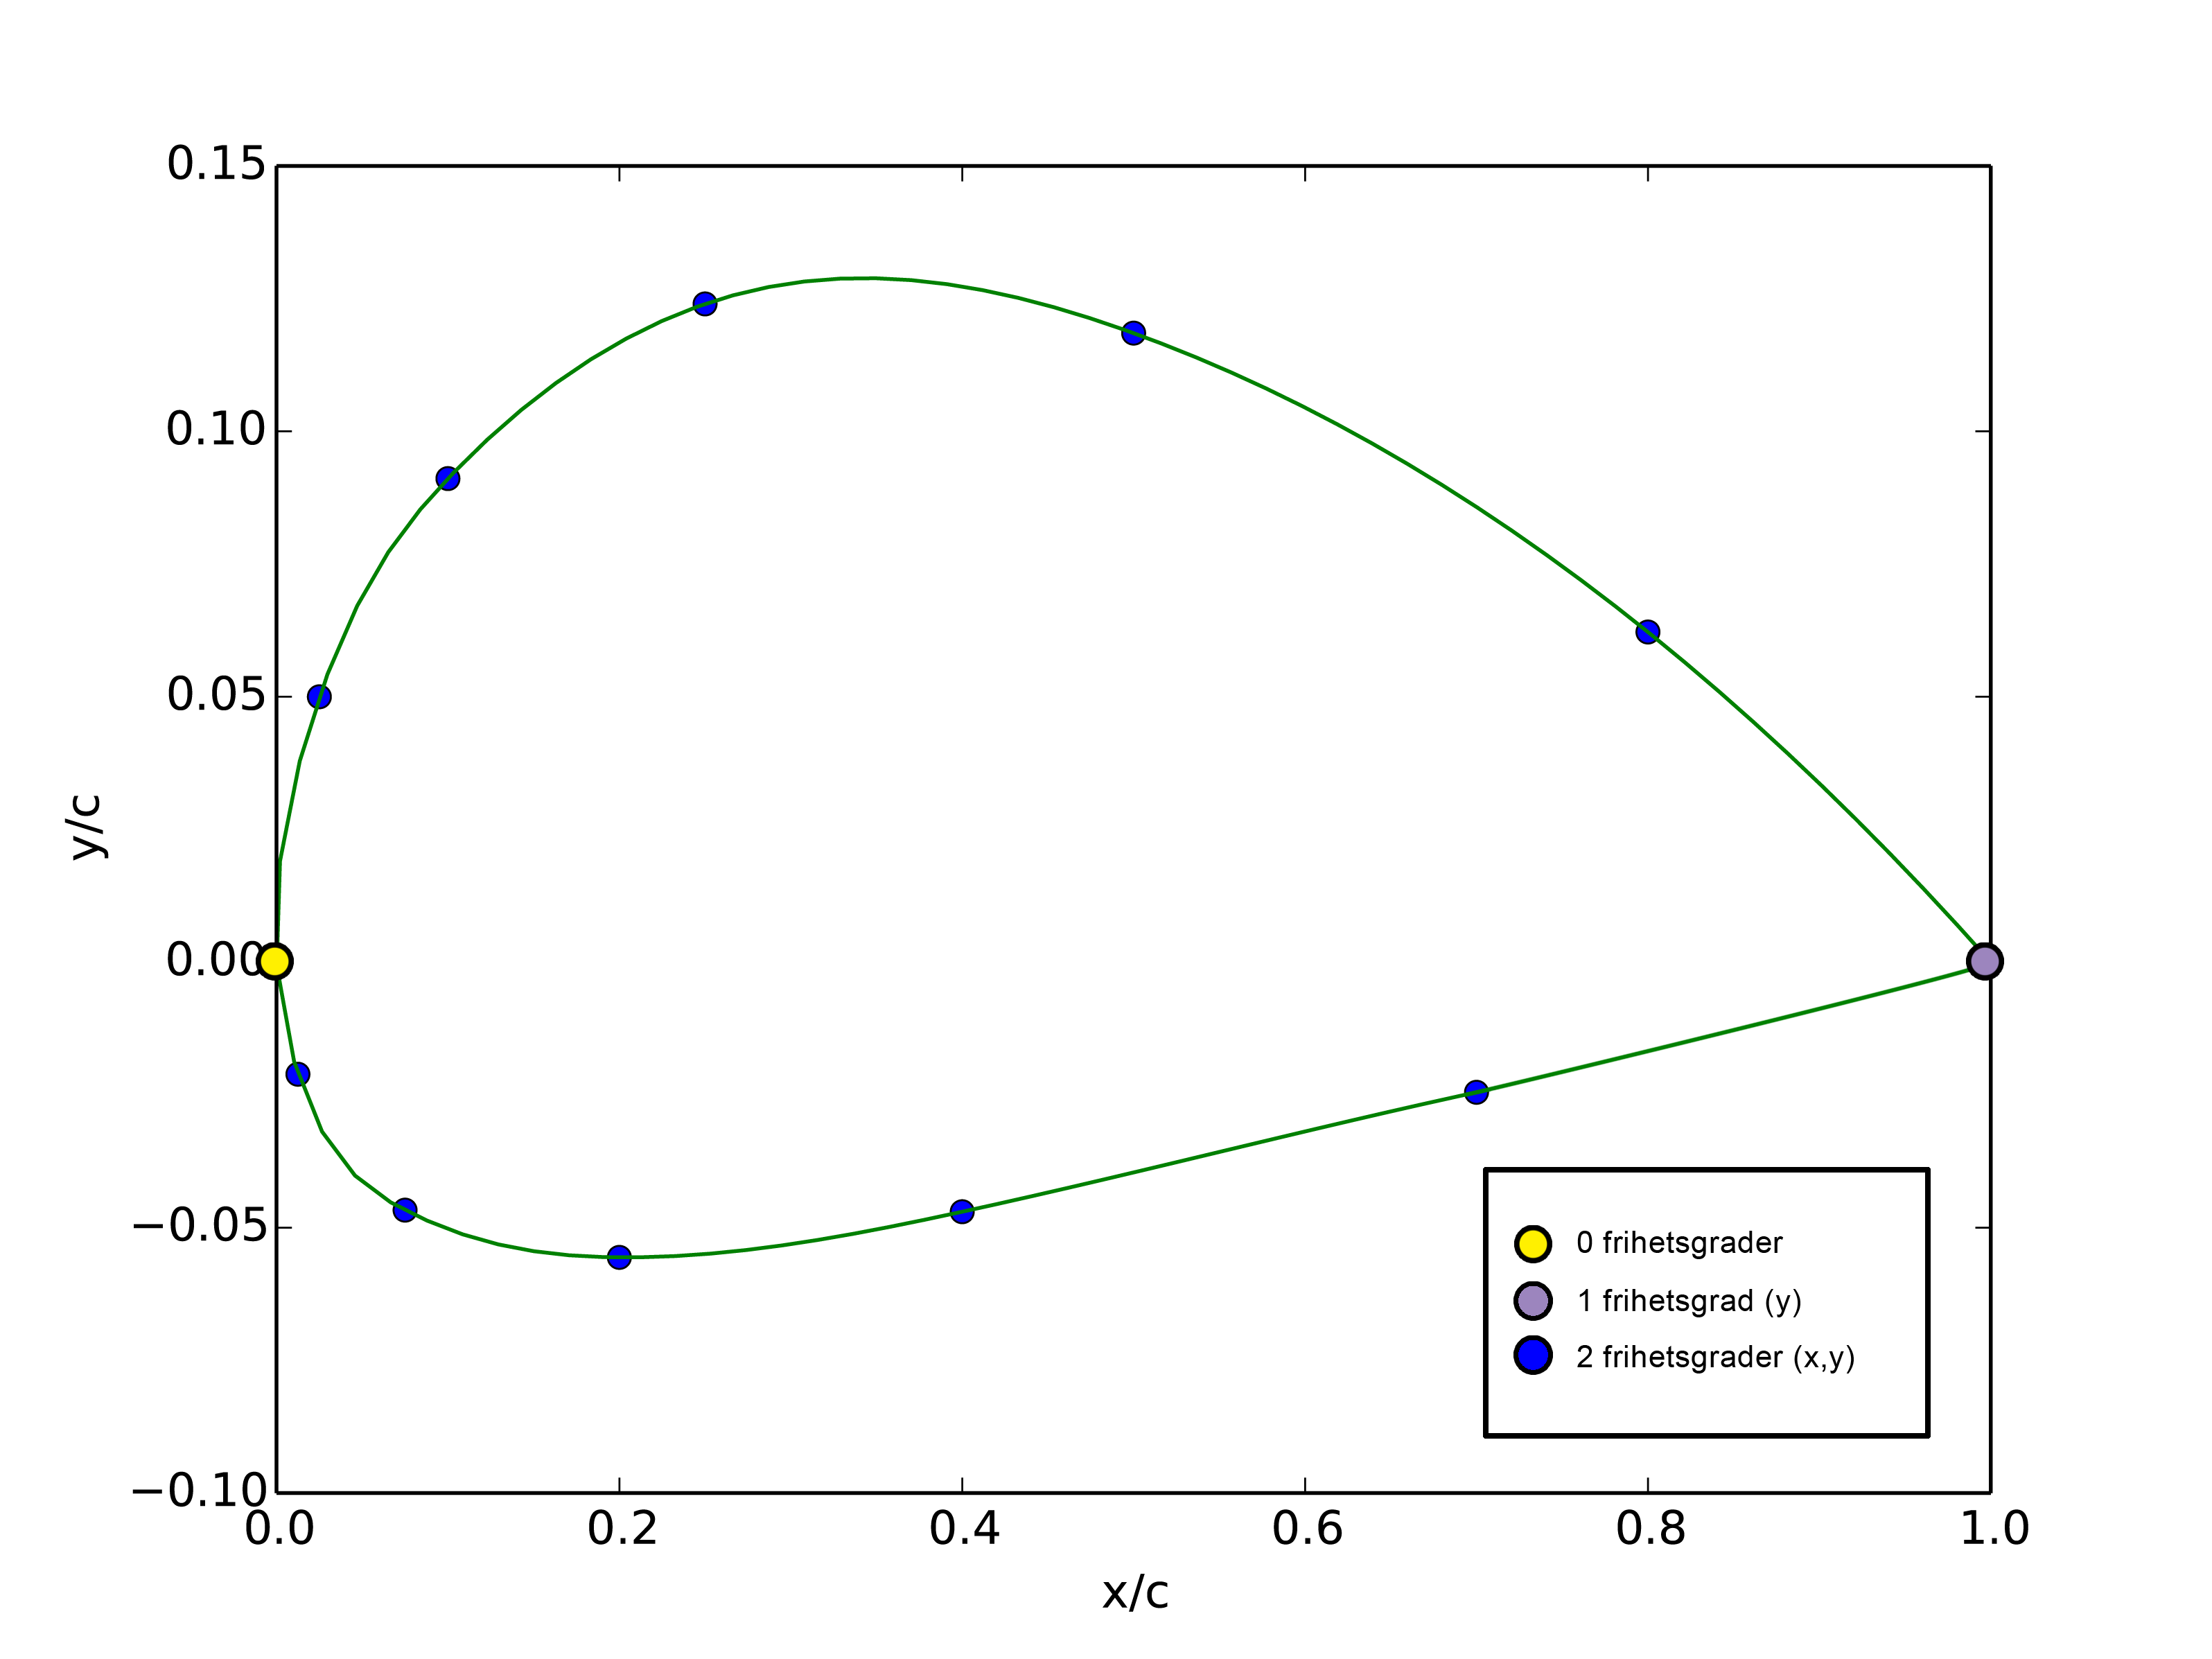
\includegraphics[width=0.47\textwidth]{bspline}
    \label{bezier-spline:left}
  }
  \subfigure[Beziér-kurva med totalt 31 frihetsgrader]{
    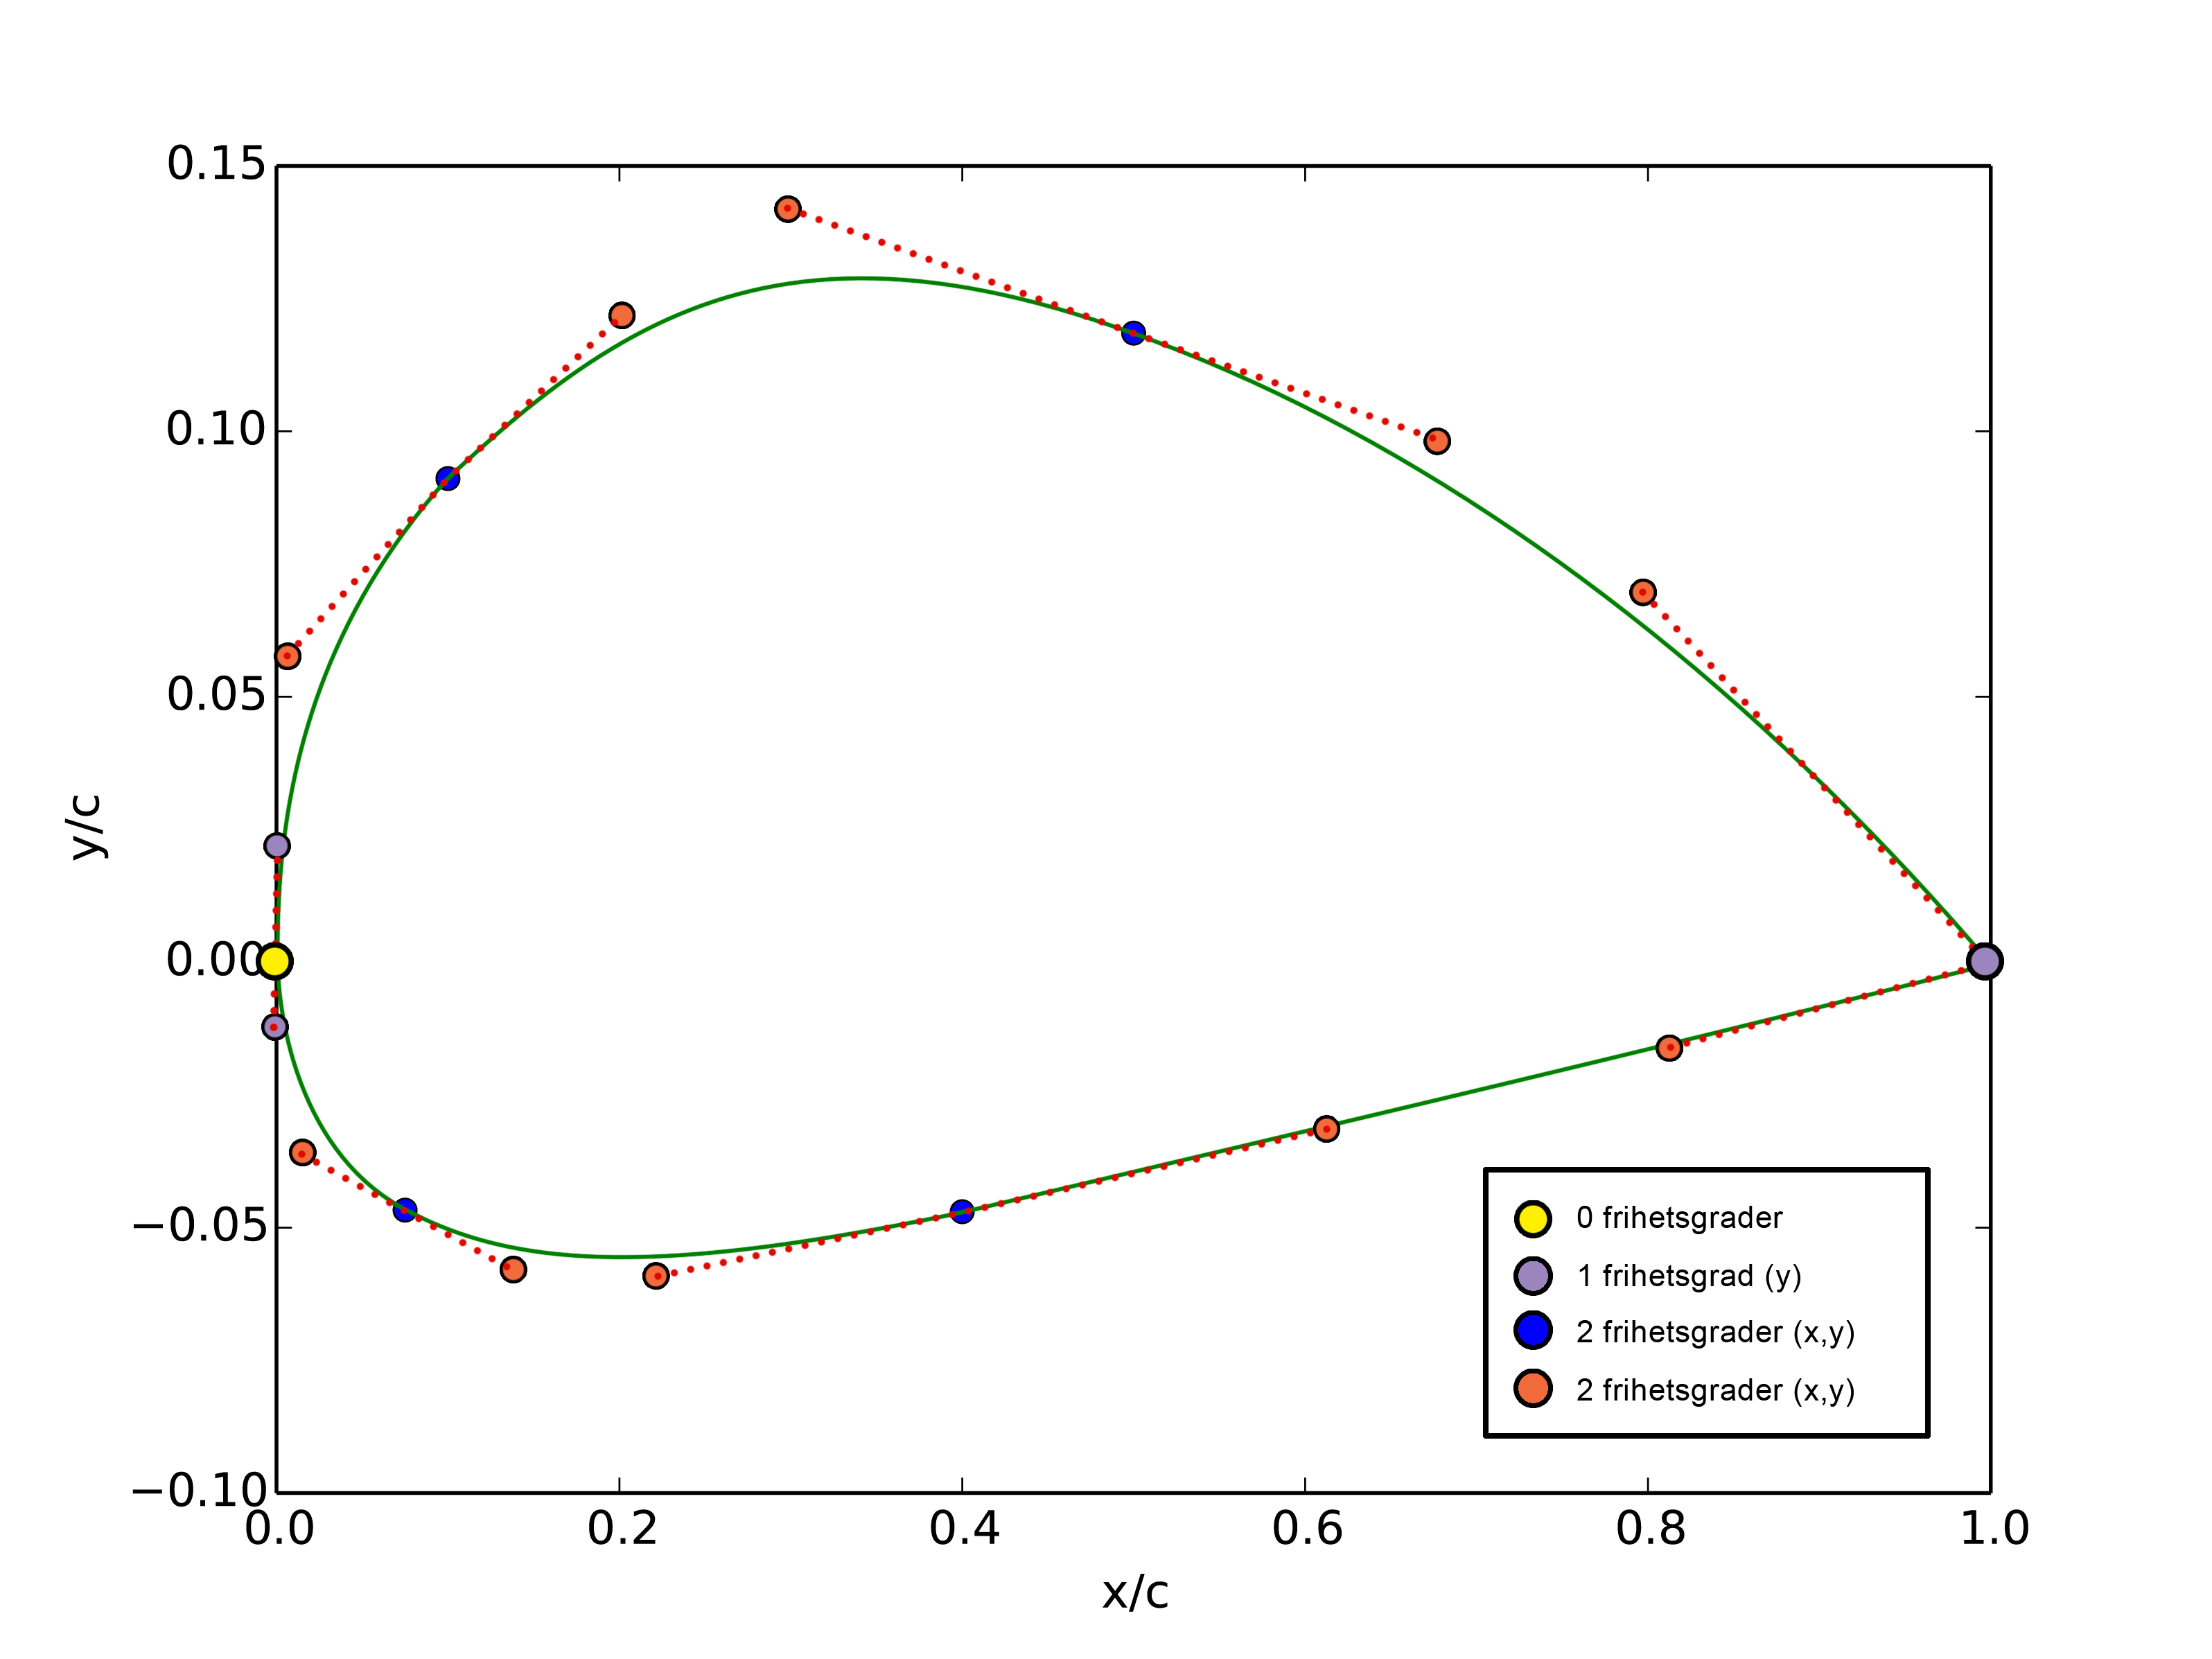
\includegraphics[width=0.47\textwidth]{bezier}
    \label{bezier-spline:right}
  }
  \caption{Jämförelse mellan B-splines och Bezier-kurvor för representation av vingprofil från diskreta punkter.}
  \label{bezier-spline}
\end{figure}

Kvar blir sammanbindning av diskreta punkter genom Beziér-kurvor eller B-splines. I \fref{bezier-spline} jämförs samma vingprofil representerad med B-spline (vänster) och en Beziér-kurva (höger). Beziérkurvan kan representeras av färre (blåa) huvudpunkter men kräver i sin tur (röda) punkter för att definiera hur kurvan mellan blåa punkter ska sammanbindas.

En B-spline är en underkategori till Beziérkurvor där punkterna som i Bezierkurvan var röda ej behöver specificeras. För att kunna styra sammanbindningen används istället fler blåa punkter.

Varje diskret punkt ger upphov till frihetsgrader i designproblemet. En punkt har oftast en frihetsgrad i x-led och en i y-led (blåa och röda punkter), men vi har även lila punkter som är begränsade till att variera endast i y-led. 

Detta illustrar sammantaget att B-spline-kurvor är en bättre vingprofilsrepresentation eftersom samma vingprofil kan åstadkommas till ett lägre antal frihetsgrader vilket syns i \fref{bezier-spline}. Därför har även denna metod valts och implementeras i mitt program med programmeringsspråket Pythons inbyggda interpoleringsmodul \lstinline[breaklines=true]!splprep!




B-splines där vingprofilens kurvatur går genom alla kontrollpunkter (parametrar). Fördel: enkelt att använda tillgängliga .dat-filer på nätet för vingprofiler. Var ett lätt sätt att komma igång. Bezier ser också ut att vara ett väldigt bra alternativ som producerar väldigt mjuka kurvor.

Minsta möjliga antal designparametrar utan att inte kunna representera alla tänkbara vingprofiler

Mycket föreslaget i litteraturen men jag fastnade för B-splines eftersom de går genom punkterna till skillnad från bezier. Detta gjorde det enkelt att under arbetes gång arbeta med vingprofiler tillgängliga på nätet som enkelt kunde översättas till sådana punkter.

Moturs definierat

nos och tail är fixerade


201 points enl 5wkillen

minst 120 enl drela gammal

därför har jag kört 200

allt mindre än panelantalet försvinner. ska därför inte sättas  för lågt

\end{comment}



\subsection{Restriktioner}

Negativ tjocklek (vingprofilens överdel korsar underdelen) är ej realistiskt och kan heller ej utvärderas i \textsc{Xfoil}. Därför subtraheras de y-värden som hör till vingprofilens underdels punkter från de på överdelen. Om ett negativt värde påträffas tilldelas vindkraftverket en negativ effekt.

\citet{Victoria} har satt minsta tjocklek på vingprofilen till 6 \% av kordan och maximal till 20 \% vilket även används i denna rapporten. 

\pagebreak

\section{Korda- och twistdistribution över bladet}

Likt vindprofilsrepresentationen ges korda- och twistdistributionen av diskreta punkter vars mellanliggande punkter interpoleras fram. Detta tas som tidigare i \ref{b-splines} fram med \lstinline[breaklines=true]!splprep! men denna gång med \lstinline[breaklines=true]!k=2!, alltså ett andragradspolynom sammanbinder punkterna. I \fref{twistdist} syns hur tre punkter utgör twist-distributionen längs rotorbladets radie. Första punkten är låst i x-ledd vid $x = 0$ och sista vid $x = 1$. Samma gäller för \fref{kordadist} där korda-distribution representeras på samma sätt.

\begin{figure}[!h]
  \centering
  \subfigure[Twist-distribution längs rotorbladets radie interpolerat från tre diskreta punkter utmarkerade i figuren.]{
    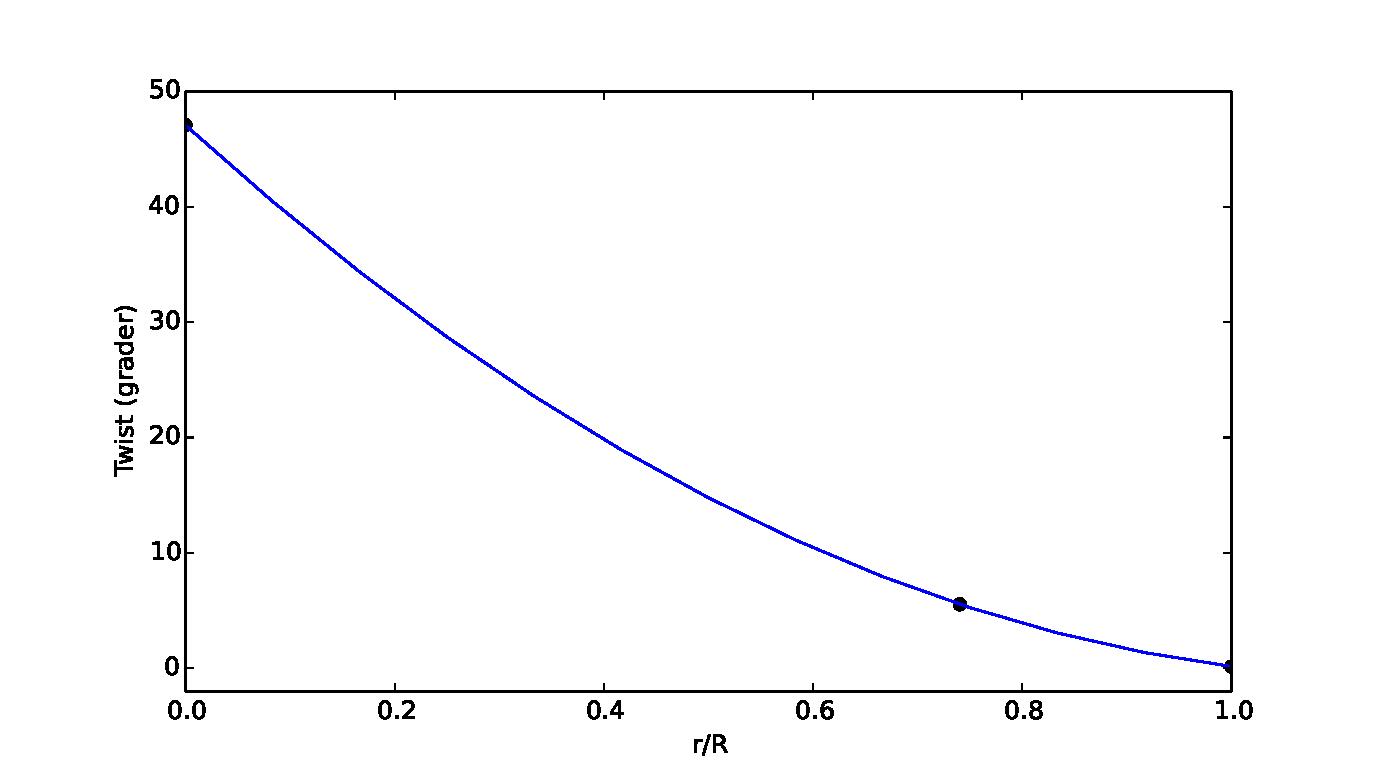
\includegraphics[width=0.8\textwidth]{twistdist}
    \label{twistdist}
  }
  \subfigure[Korda-distribution längs rotorbladets radie interpolerat från tre diskreta punkter utmarkerade i figuren.]{
    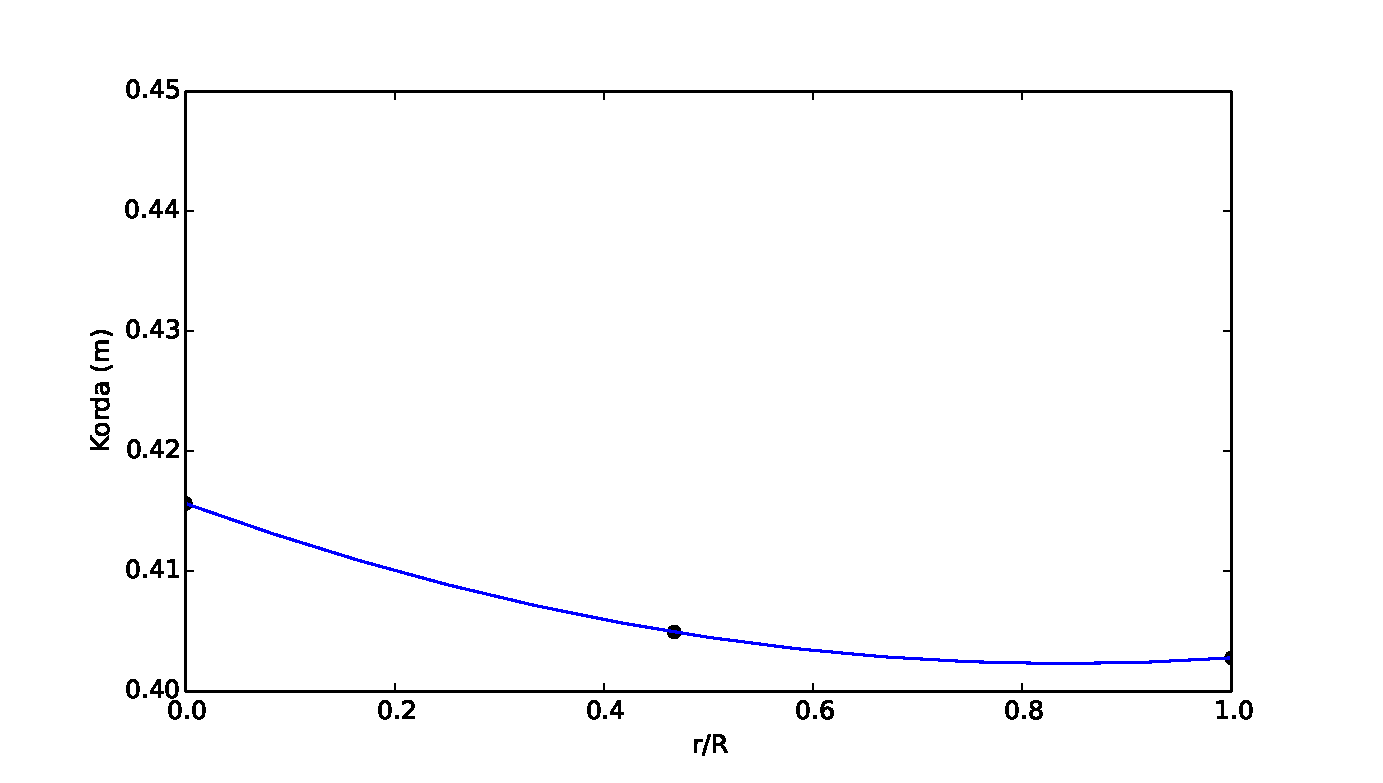
\includegraphics[width=0.8\textwidth]{kordadist}
    \label{kordadist}
  }
  \caption{Korda- respektive twistdistribution över bladet}
  %\label{hawtvawt}
\end{figure}


\subsection{Restriktioner}

Maximal och minimal korda och twist från \citet{Victoria} ses i \tref{kordatwistvictoria}.

\bigskip
\begin{table}[!htb]

\small
%\bigskip
  \centering
  
    \begin{tabular}{lll}
    
    \toprule
    Parameter & Max-värde & Min-värde \\
    \midrule
    \citet{Victoria} korda & 0.40 m & 0.05 m \\
    Vald korda för studien & 1.60 m & 0.10 m \\
    
    Twist & 75$^{\circ}$ & -75$^{\circ}$ \\
    \bottomrule
    \end{tabular}
  \caption{Maximal och minimal korda och twist enligt  \citet{Victoria} samt valda värden för studien.}
  \label{kordatwistvictoria}
\end{table}

I denna studie kommer senare ett vindkraftverk med c:a 10 meters diameter beaktas. Eftersom \citet{Victoria} behandlade ett vindkraftverk med c:a 5 meter i diameter har min-värdet för kordan satts till det dubbla och max-värdet det fyrdubbla.


\section{Rotorbladsrepresentation}

\begin{figure}[!htb]
  \centering
  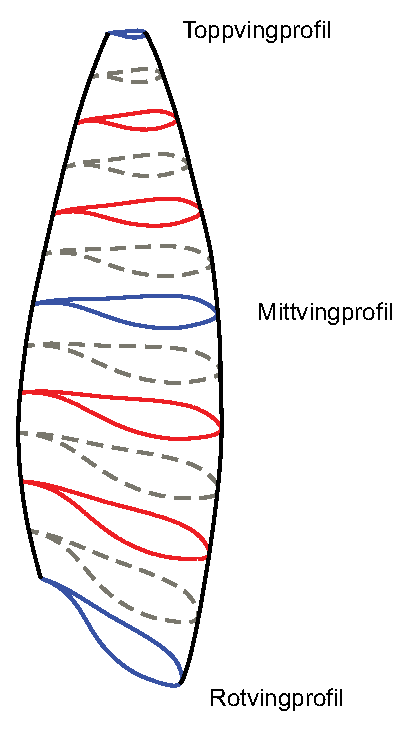
\includegraphics[height=10cm]{vinge_tjock_p.eps}
  
  \caption{Rotorbladets representation i SiteOpt}
  \label{rotmellantopp}
\end{figure}

Rotorbladet består i modellen av tre huvudsakliga vingprofiler. En vingprofil som ligger där rotorbladet börjar (rotvingprofil), en vingprofil vid rotorbladets topp (toppvingprofil) samt en mellanliggande (mittvingprofil). Se \fref{rotmellantopp}. Dessa är således även vingprofilerna vars geometri som i optimeringen varieras.

Ur dessa huvudsakliga vingprofiler interpoleras fyra ytterligare mellanliggande profiler. Två mellan rot-mitt och två mellan mitt-topp vilka även syns i \fref{rotmellantopp} som streckade röda vingprofiler. 

I \fref{connectTheDots2} visades att vingprofilerna byggs upp av 12 diskreta punkter. Om varje sådan punkt betecknas

\begin{equation*}
s_i = \begin{pmatrix}
x_i \\
y_i
\end{pmatrix}
\end{equation}

och vingprofilerna som ska interpoleras mellan är A och B med respektive uppsättning punkter $\mathbf{S}_A = \left\{ s_1, \dots, s_{12}\right\}_A$ och $\mathbf{S}_B = \left\{ s_1, \dots, s_{12}\right\}_B$ ges de linjärt mellanliggande punkterna $\mathbf{S}_I$ av

\begin{equation*}
\mathbf{S}_{I} = \mathbf{S}_A\left(\mathbf{S}_B - \mathbf{S}_A\right)\Delta H
\end{equation}

Där $\Delta H$ är i procent hur mycket $ \mathbf{S}_B$ ska blandas i $ \mathbf{S}_A$. Detta resulterar alltså totalt i fyra nya vingprofiler som utvärderas i \textsc{Xfoil} (utmarkerad som röda streckade i \fref{rotmellantopp}). 

$C_l$ och $C_d$-kurvorna för vingprofilerna kan nu interpoleras linjärt mellan de alla de vingprofilerna som utvärderats i \textsc{Xfoil} och sex mellanliggande positioner tas fram vilket i \fref{rotmellantopp} är utmarkerat som långt streckade gråa element.

Rotorbladet har nu 13 vingprofiler och består av 12 radiella element.

I SiteOpt har användaren valet att om önskat stänga av vingprofilsinterpoleringen eftersom den leder till fler anrop till \textsc{Xfoil} och därmed mer beräkningstid. Då görs istället en linjär interpolering av $C_l$ och $C_d$ för alla radiella positioner mellan huvudvingprofilerna (rot, mellan och topp).

\section{SiteOpts implementering av \textsc{Bem}}
\label{siteoptBEM}
\textsc{Bem}-modellen har implementerats som beskrivet i litteraturstudien (se \ref{BEMlitt}). Följande mer specifika implementeringar för SiteOpt presenteras här:

\begin{itemize}

\item När $a$ och $a'$ beräknas görs maximalt 200 iterationer innan algoritmen avslutas. Om feltoleransen $10^{-4}$ uppnås innan det, avslutas iterationen då. 

\item För att en diskontinuitet i \textsc{Bem} beskriven i \citet{damp} inte ska bli ett problem används en dämpade faktor satt till 0.5 när $a$ och $a'$ uppdateras i varje iteration. $a$ och $a'$ uppdateras alltså endast 50 \% i den riktning ett nytt värde räknats ut.

\item Algoritmen har tillgång till $C_l$ och $C_d$ för alla vingprofiler i rotorbladet vid önskad angreppsvinkel $\alpha$ och $Re$ genom interpolation som beskrivs senare i \ref{clinterpol}. För att möjliggöra detta beräknas

\begin{equation*}
V_{tot} = \sqrt{ \left(V_{\infty}\left(1 - a\right)\right)^2 + \left(\Omega r \left(1 + a'\right)\right)^2} 
\end{equation*}

vilket erhålls genom geometrin i \fref{vrotva}. Med $V_{tot}$ kan nu $Re$ beräknas över sin definition så att \textsc{Xfoil} kan utvärdera vid rätt $Re$.

\item Ett $Re_{max}$ och $Re_{min}$ behöver tas fram för att modellen ska veta mellan vilka $Re$ som \textsc{Xfoil} ska kallas. $Re_{max}$ och $Re_{min}$ tas fram som

\begin{equation*}
\begin{array}{cc}
Re_{max} = \frac{\sqrt{U_{ut}^2 + \left(\lambda U_{ut}\right)^2}c_{max}}{\nu}, & Re_{min} = \frac{\sqrt{U_{in}^2 + \left(\lambda U_{in}\right)^2}c_{min}}{\nu}\\ 
\end{array}
\end{equation*}


$N_{Re}$ st antal $Re$ tas sedan fram mellan $Re_{max}$ och $Re_{min}$. Användaren har dock även valet att välja att endast ett specificerat $Re$ utvärderas.

\item Kunde inte $C_l$ och $C_d$ erhållas från \textsc{Xfoil} sätts \textsc{Bem}-modellens resultat till en negativ effekt vilket resulterar i att den kommer sorteras bort av den genetiska algoritmen.

\end{itemize}


\subsection{Fixerade parametrar}

\textsc{Bem} kräver även ytterligare parametrar, fysikaliska storheter och toleransnivåer som är fixerade och ej varieras i optimeringen. Dessa ställs in genom att editera de första raderna på SiteOpt.

\begin{itemize}
\item Märkeffekt (eng: rated power)
\item Bladets toppradie ($R$)
\item Bladets startradie ($r_{hub}$) mätt från rotationsaxeln
\item Löptal $\lambda$ (eller vid konstant rotationshastighet $RPM$)
\item Inkopplingshastighet ($U_{in}$)
\item Urkopplingshastighet ($U_{ut}$)
\item Antal rotorblad ($B$)
\item Pitch-vinkel ($\theta_p$)
\item Reynoldsupplösning ($N_{Re}$) - Antalet $Re$ som ska utvärderas mellan $Re_{min}$ och $Re_{max}$ av \textsc{Xfoil}. 
\item $\rho$ - Luftens densitet
\item $tol$ - Toleransnivån för $a$- och $a'$iterationen

\end{itemize}

Givet allt detta kan nu \textsc{BEMT}-metoden generera en effektkurva som kan paras med vindhastighetshistogrammet för att ge genomsnittseffekten $\overline{P}$. Detta beskrivs noggrannare i \ref{fitnessfunk}.

\section{Erhållande av $C_l$ och $C_d$}
\subsection{\textsc{Xfoil}}
\label{xfoilcomm}





\textsc{Xfoil} är en programvara som kan lösa det inviskösa och viskösa flödet kring en vingprofil utvecklat av Mark Drela och beskrivet av samma författare i \citet{Xfoil}. Detta görs genom en linjär vorticitetmetod tillsammans med Karman-Tsien-kompesibilitetskorrektion som löser det inviskösa flödet. Gränsskiktet och övergången till turbulent flöde löses simultant med det inviskösa potentialflödet med en global Newton–Raphson-metod. 

Givet en vingprofil, Reynolds tal ($Re$) och angreppsvinkel ($\alpha$) kan $C_l$, och $C_d$ erhållas för vingprofiler där formen ligger inom ramarna för hur en vingprofil brukar se ut - och där angreppsvinklarna inte avviker allt för mycket från spannet $-5 < \alpha < 30$. Hur vinklar utanför detta spannet erhålls beskrivs i \ref{post-stall}.

\textsc{Xfoil} har ett textbaserat gränssnitt som nås via kommandoraden vilket gör det enkelt att koppla samman med studiens utvecklade programvara SiteOpt. Ett exempel på vilka kommandon som används ses i \fref{xfoilinput}. Detta skapar filen \lstinline[breaklines=true]!S809.pol! innehållandes det som sedan i \fref{xfoiloutput} ses.




\lstinline[breaklines=true]!S809.pol! läses sedan av SiteOpt som en vanlig textfil och får på så sätt få tillgång till $C_l$ och $C_d$.

\textsc{Xfoil} kommer för vissa $\alpha$ inte uppnå konvergens och av den anledning hoppa över den vinkeln. Detta går att lösa genom att låta \textsc{Xfoil} iterera ytterligare gånger när detta sker. Men eftersom detta skulle addera ytterligare beräkningstid  interpoleras istället gällande värden fram linjärt mellan de närliggande värdena.   

\textsc{Xfoil} låter användaren specificera $N_{crit}$ vilket är att tolkas som turbulensnivån på flödet. Detta har i studien satts till standardvärdet 9.

\begin{figure}[!h]
  \centering
    \begingroup
    \fontsize{10pt}{12pt}\selectfont
    \begin{verbatim}
    
    LOAD S809.dat
    PANE
    PANE
    OPER
    VPAR 
    N 9
    VISC 1e6
    ITER 50
    PACC
    S809.pol
    ASEQ -1 20 1
    PACC
    QUIT
    \end{verbatim} 
    \endgroup
  \caption{Exempel på input skickad till \textsc{Xfoil}.}
  \label{xfoilinput}
  
\end{figure}  

\begin{figure}[!h]
 \bigskip\bigskip

    \begingroup
    \fontsize{10pt}{12pt}\selectfont
    \begin{verbatim}

       alpha    CL        CD       CDp       CM     Top_Xtr  Bot_Xtr
      ------ -------- --------- --------- -------- -------- --------
      -1.000  -0.0083   0.00808   0.00258  -0.0326   0.6020   0.5241
       0.000   0.1114   0.00823   0.00279  -0.0351   0.5982   0.5427
       1.000   0.2308   0.00839   0.00304  -0.0375   0.5937   0.5556
       2.000   0.3499   0.00854   0.00318  -0.0399   0.5855   0.5619
       3.000   0.4676   0.00825   0.00298  -0.0419   0.5686   0.5686
       4.000   0.5844   0.00813   0.00294  -0.0437   0.5388   0.5747
       6.000   0.7398   0.01399   0.00672  -0.0367   0.0361   0.5865
       7.000   0.8201   0.01591   0.00880  -0.0332   0.0281   0.5928
       8.000   0.8913   0.01754   0.01051  -0.0287   0.0253   0.5976
       9.000   0.9412   0.02155   0.01474  -0.0246   0.0224   0.6048
      10.000   1.0064   0.02545   0.01879  -0.0237   0.0206   0.6115
      11.000   1.0604   0.03032   0.02374  -0.0224   0.0189   0.6170
      12.000   1.0951   0.03646   0.03014  -0.0196   0.0177   0.6242
      13.000   1.1385   0.04198   0.03584  -0.0177   0.0165   0.6310
      14.000   1.1792   0.04804   0.04204  -0.0164   0.0155   0.6380
      15.000   1.2049   0.05550   0.04977  -0.0142   0.0146   0.6451
      16.000   1.2338   0.06347   0.05802  -0.0135   0.0140   0.6516
      17.000   1.2545   0.07277   0.06767  -0.0139   0.0133   0.6607
      18.000   1.2668   0.08370   0.07888  -0.0156   0.0128   0.6683
      19.000   1.2663   0.09671   0.09217  -0.0186   0.0123   0.6765
      20.000   1.2378   0.11476   0.11077  -0.0246   0.0119   0.6842
    \end{verbatim}
    \endgroup
  \caption{Exempel på output som \textsc{Xfoil} returnerar i form av en textfil.}
  \label{xfoiloutput}
\end{figure}

\pagebreak 
\subsection{Interpolering mellan olika $Re$ och $\alpha$ för $C_l$ och $C_d$}
\label{clinterpol}

Proceduren beskriven i \ref{xfoilcomm} behöver göras en gång för varje $Re$ som önskas. 

När flera $Re$ utvärderats finns alltså data likt det som syns i \fref{xfoilscatter} i diskreta punkter. För att \textsc{Bem}-modellen ska kunna erhålla $C_l$ för vilket $Re$ och $\alpha$ som helst görs en linjär interpolering i två dimensioner mellan de närmsta värdena. På samma sätt görs för $C_d$.

Har endast ett $Re$ valts görs interpolationen endast på $\alpha$ och oberoende av $Re$.

\begin{figure}[!h]
  \centering
  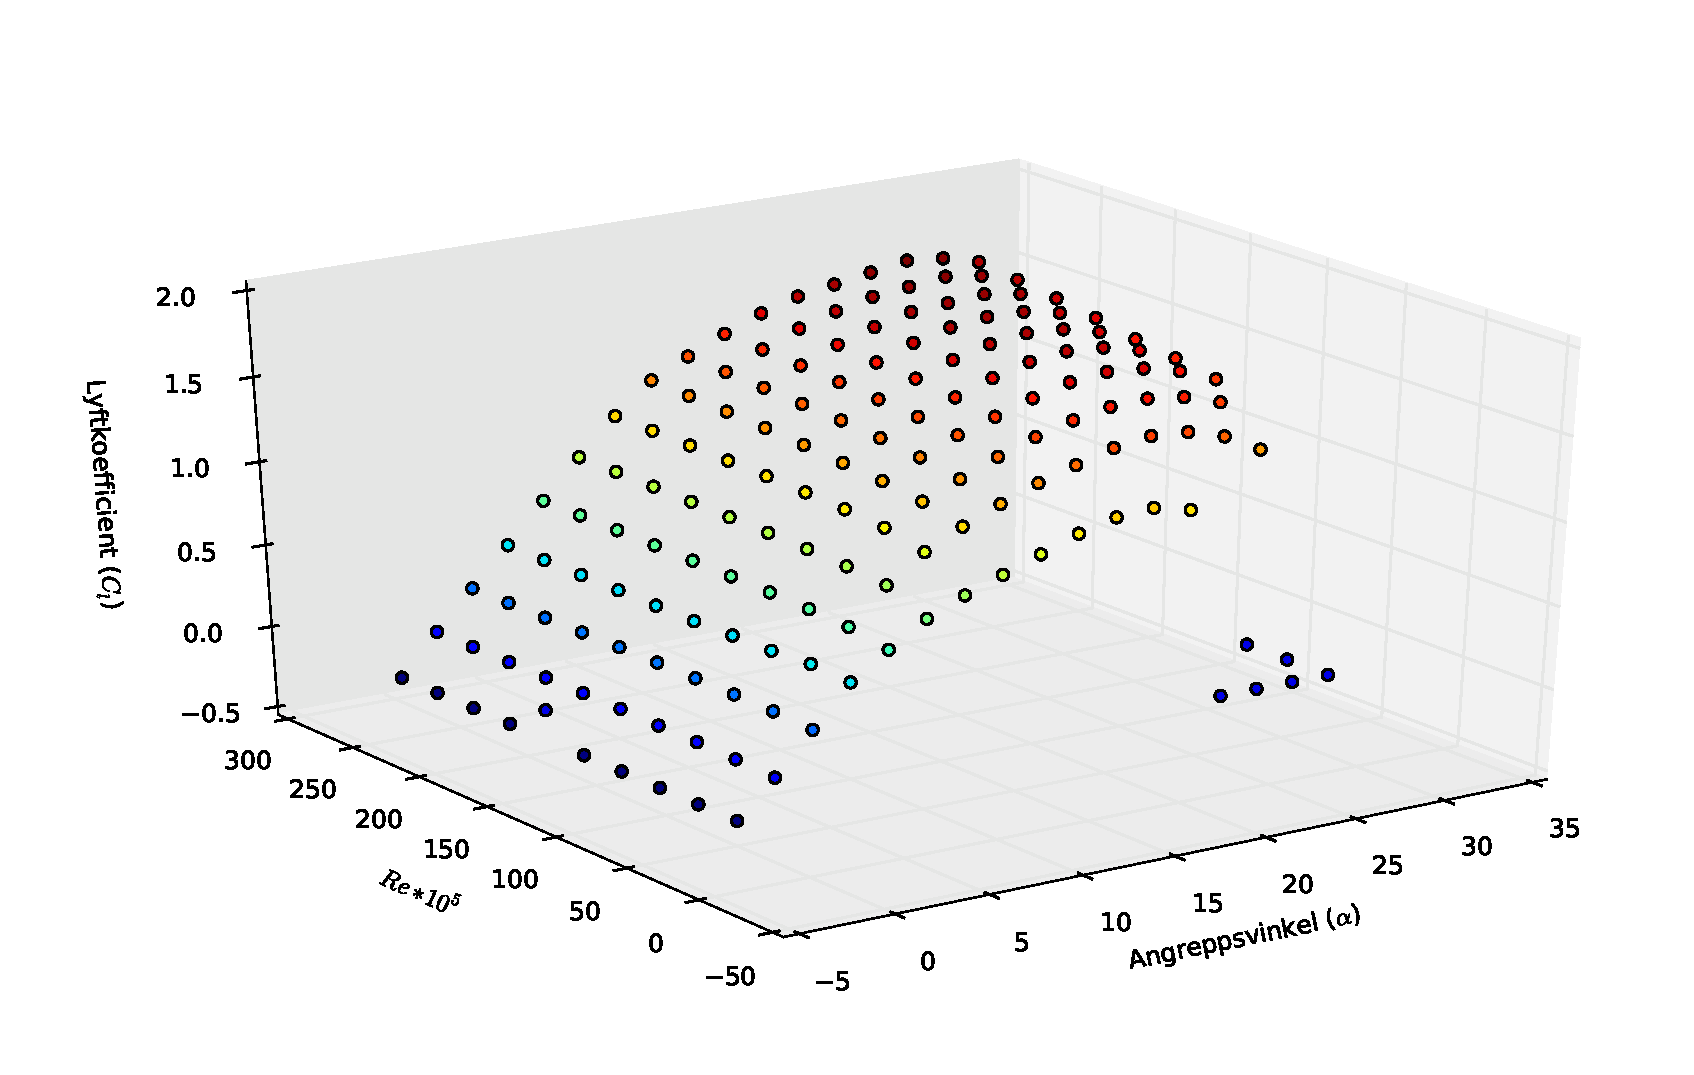
\includegraphics[width=1\textwidth]{Re_Alfa-map_scatter}
  \caption{Resulterande $C_l$ efter utvärdering av 10 st $Re$ i \textsc{Xfoil}}
  \label{xfoilscatter}
\end{figure}

\subsection{Hantering av uteblivet resultat från \textsc{Xfoil}}

För vissa $Re$ lyckas \textsc{Xfoil} inte ge något resultat över huvud taget. Detta hanteras genom att det problematiska $Re$ ignoreras och istället interpoleras mellanliggande fram som beskrivet i \ref{clinterpol}.

Det händer även att \textsc{Xfoil} låser sig. Exakt när detta sker och varför har inte kunnat kartläggas helt men beror förmodligen på en för avvikande vingprofil. För att kunna hantera detta har en timer implementerats. Har inget resultat kommit från \textsc{Xfoil} efter 60 sekunder får vingprofilen tilldelat sig negativa $C_l$ och $C_d$ för att på så sätt rensas ut.

\section{Post-stall-extrapolation av $C_d$ och $C_l$}
\label{post-stall}

\textsc{Xfoil} ger endast tillförlitliga resultat fram till $\alpha_{stall}$ \citep{XfoilVerifikation}. Av den anledningen har endast angreppsvinklarna $-5^{\circ} < \alpha < 30^{\circ}$ utvärderats med \textsc{Xfoil}. Därefter har $\alpha_{stall}$ satts till det $\alpha$ där $C_l$ haft högst värde ($C_{l_{stall}}$).

\textsc{Bem}-algoritmen behöver i vanliga fall inga $C_l$ och $C_d$ utanför  $-5^{\circ} < \alpha < \alpha_{stall}$. Men i undantagsfall och under optimeringsprocessen behövs $\alpha$ utanför intervallet. Därför har Viternaekvationerna implementerats vilka beskriver ett enkelt sätt att extrapolera $C_l$ och $C_d$ utanför intervallet. Detta beskrivs i \citet{viterna} och återges här i korthet.

Extrapoleringen av $C_d$ görs för intervallet $\alpha_{stall} < \alpha < 90^{\circ}$ görs med 

\begin{equation}\label{Cd} 
C_{d} = B_1\sin ^2\alpha + B_2\cos\alpha
\end{equation}

där 

\begin{subequations}
\label{ARB1B2}  
\begin{align}
        AR &= \frac{R}{c_{0.8R}}\\
        B_1 &= C_{d_{max}} = 1.11 + 0.018AR\\
        B_2 &= \frac{C_{D_{stall}}-C_{D_{max}}\sin^2\alpha_{stall}}{\cos\alpha_{stall}}
\end{align}
\end{subequations}

$AR$ är ett förhållande mellan radien och kordan ($c$) vid 80 \% av radien ($c_{0.8R}$). 

På liknande sätt kan $C_l$ extrapoleras i $\alpha_{stall} < \alpha < 90^{\circ}$ med

\begin{equation}\label{CL} 
C_l= A_1\sin2\alpha + A_2\frac{\cos^2\alpha}{\sin\alpha}
\end{equation}

där

\begin{subequations}
\label{A1A2}  
\begin{align}
        A_1 &= B_1/2\\
        A_2 &= (C_{l_{stall}}-C_{d_{max}}\sin\alpha_{stall}\cos\alpha_{stall})\frac{\sin\alpha_{stall}}{\cos^2\alpha_{stall}}
\end{align}
\end{subequations}

Ytterligare $C_l$ och $C_d$ kan extrapoleras med antagandet att vingprofilen beter sig som en platt platta i intervallet $ 90^{\circ} < \alpha < 180^{\circ}$ positivt och negativt


\begin{subequations}
\label{plattor} 
\begin{align}
        C_{L_{platta}} &= 2\sin\alpha\cos\alpha\\
        C_{D_{platta}} &= B_1\sin^2\alpha
\end{align}
\end{subequations}

Genom dessa ekvationer och datan från \textsc{Xfoil} kan nu $C_l$ och $C_d$ erhållas för $-180^{\circ} < \alpha < 180^{\circ}$. I \fref{clinterpolfig} syns datan från \textsc{Xfoil} i en tjockare blå linje medans den extrapolerade är den tunnare gröna linjen.

$C_d$ tas på samma sätt fram för hela spannet. I \fref{cdinterpolfig} syns \textsc{Xfoil}s data med tjock blå linje och den extrapolerade med tunn grön linje.


\begin{figure}[!h]
  \centering
  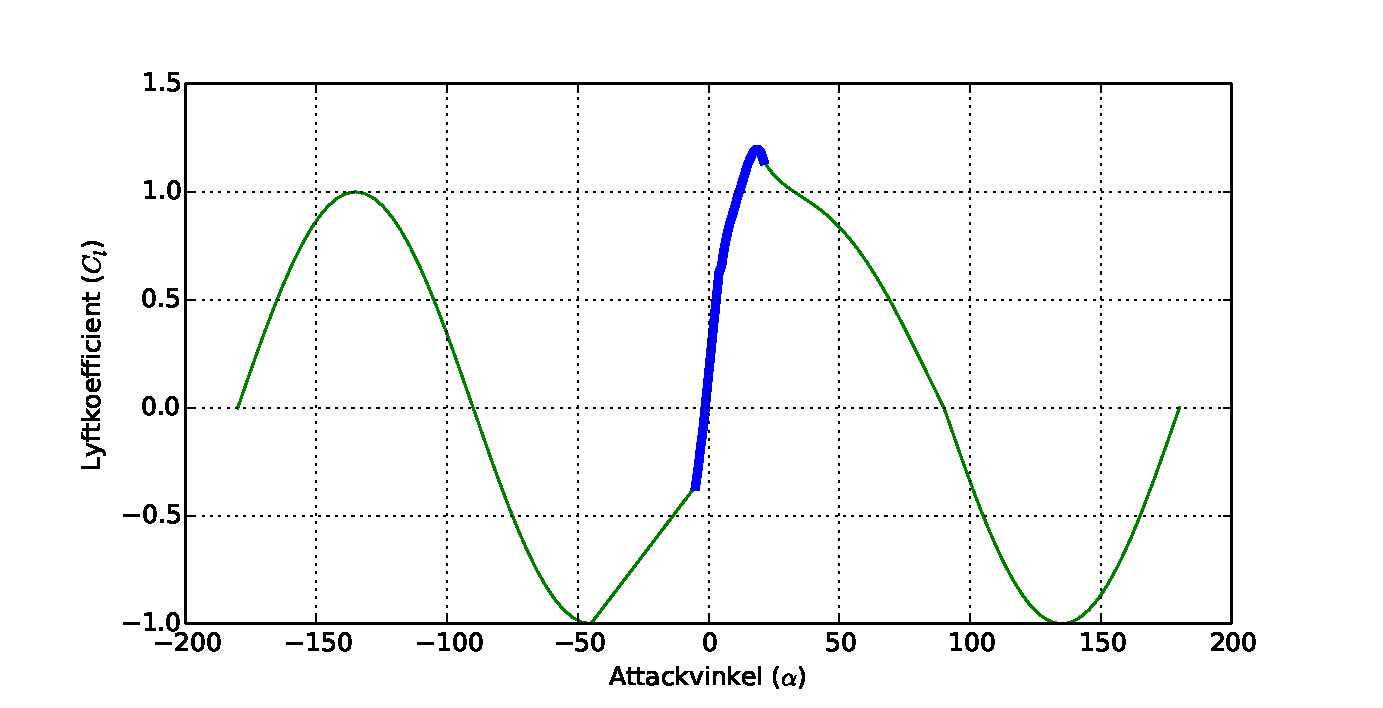
\includegraphics[width=0.9\textwidth]{liftinterpol}
  \caption{$C_l$ från \textsc{Xfoil} (fet linje) och extrapolerade $C_l$ (tunn linje) enligt förfarandet beskrivet i \ref{clinterpol} för en S809 vingprofil vid $Re$ en miljon. }
  \label{clinterpolfig}
\end{figure}


\begin{figure}[!h]
  \centering
  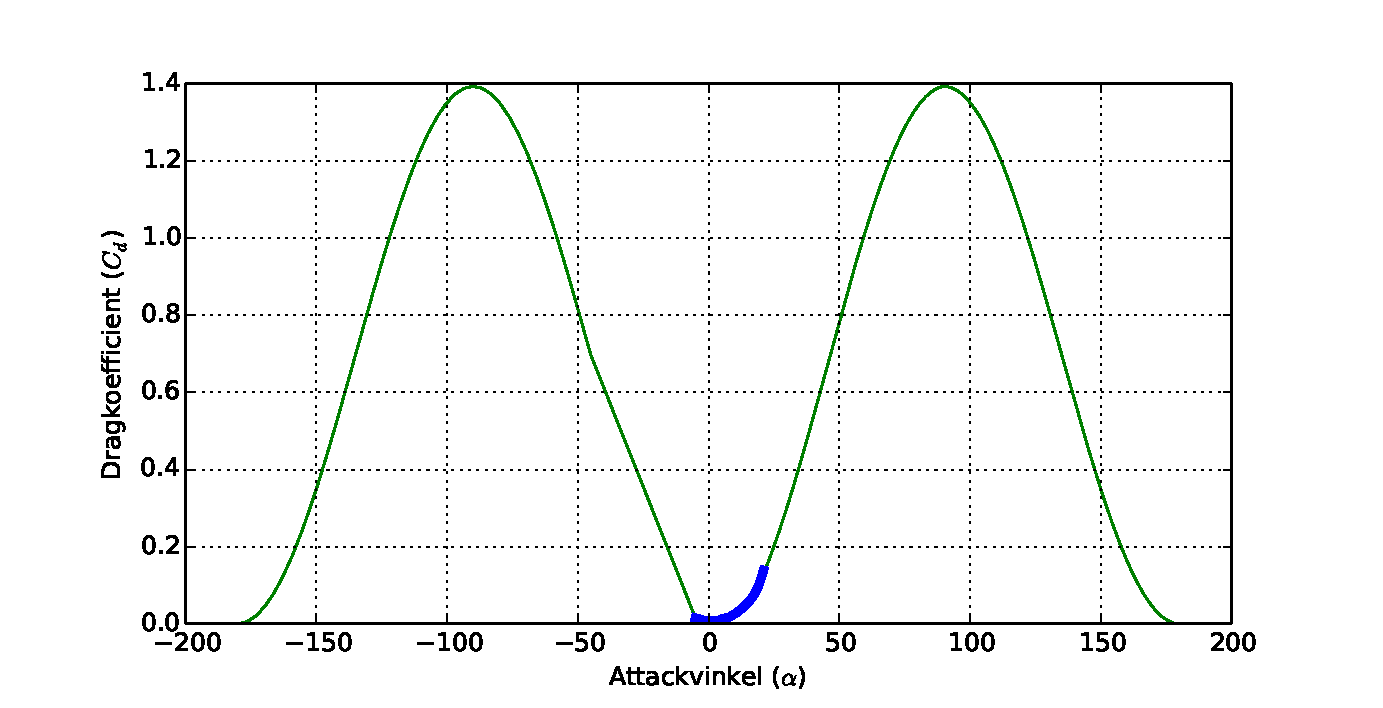
\includegraphics[width=0.9\textwidth]{draginterpol}
  \caption{$C_d$ från \textsc{Xfoil} (fet linje) och extrapolerade $C_d$ (tunn linje) enligt förfarandet beskrivet i \ref{clinterpol} för en S809 vingprofil vid $Re$ en miljon. }
  \label{cdinterpolfig}
\end{figure}







\section{Vindhastighetsprofiler}
\label{vindhastighetsprofiler}


SiteOpt tar som input en vindhastighetsprofil - det vill säga ett histogram över förekomsten av olika vindhastigheter för en plats. Data från St. Lawrence i Kanada \citep{Victoria} syns i \fref{vindprofil} (mätt 30 meter från marken). Antalet observationer har normerats till en procentuell förekomst. Summan av alla staplar är således 1.

Detta histogram används sedan i referensfallet och kallas vidare $h(U)$ (där $U$ är en vindhastighet) och används som uppskattning av den bakomliggande sannolikhetsfördelningen (vidare kallad $f_w(U)$). 

\begin{figure}[!htb]
  \centering
  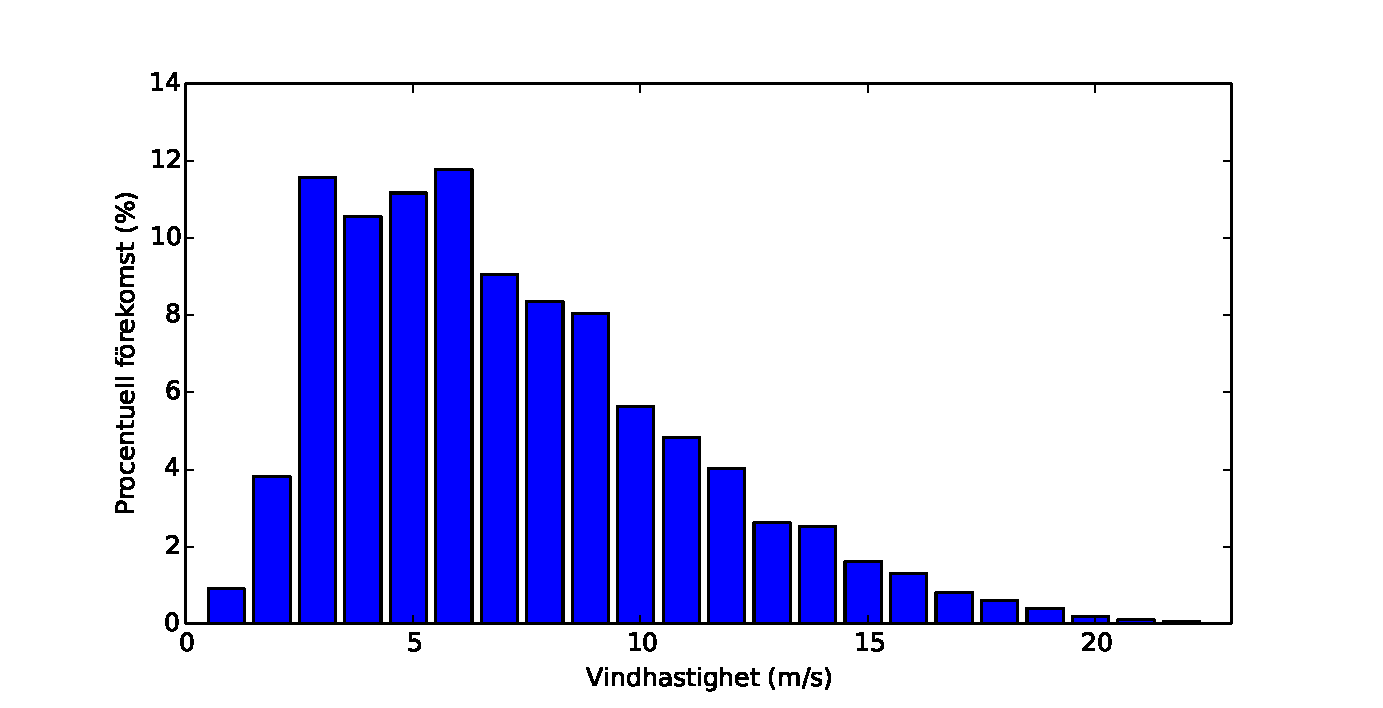
\includegraphics[width=0.9\textwidth]{vindprofil}
  \caption{Vindhastighetsfördelning. Data från hämtad från St. Lawrence i Canada  reproducerad från \citet{Victoria}.}
  \label{vindprofil}
\end{figure}

\pagebreak

\section{Genetisk algoritm}

När den genetiska algoritmen initieras så skapas en första population. Denna utgår från vingprofilen S809 varpå de diskreta punkterna som bygger upp vingprofilen utsätts för en gaussisk slumpfaktor med standardavvikelse om 10 \% från de ursprungliga punkterna som bygger upp S809. Detta görs för att skapa en population med vingprofilskaraktär samtidigt som en bred del av designrymden söks av.

I \fref{initpop} visas den initiala populationens 28 första rot-vingprofiler som exempel, men populationen kan alltså även innehålla mellan-vingprofilen, top-vingprofilen, kordadistributionen och twistdistributionen som här ej visas. Dessa utsätts för samma slumpade initiering.

\begin{figure}[!htb]
\bigskip
  \centering
  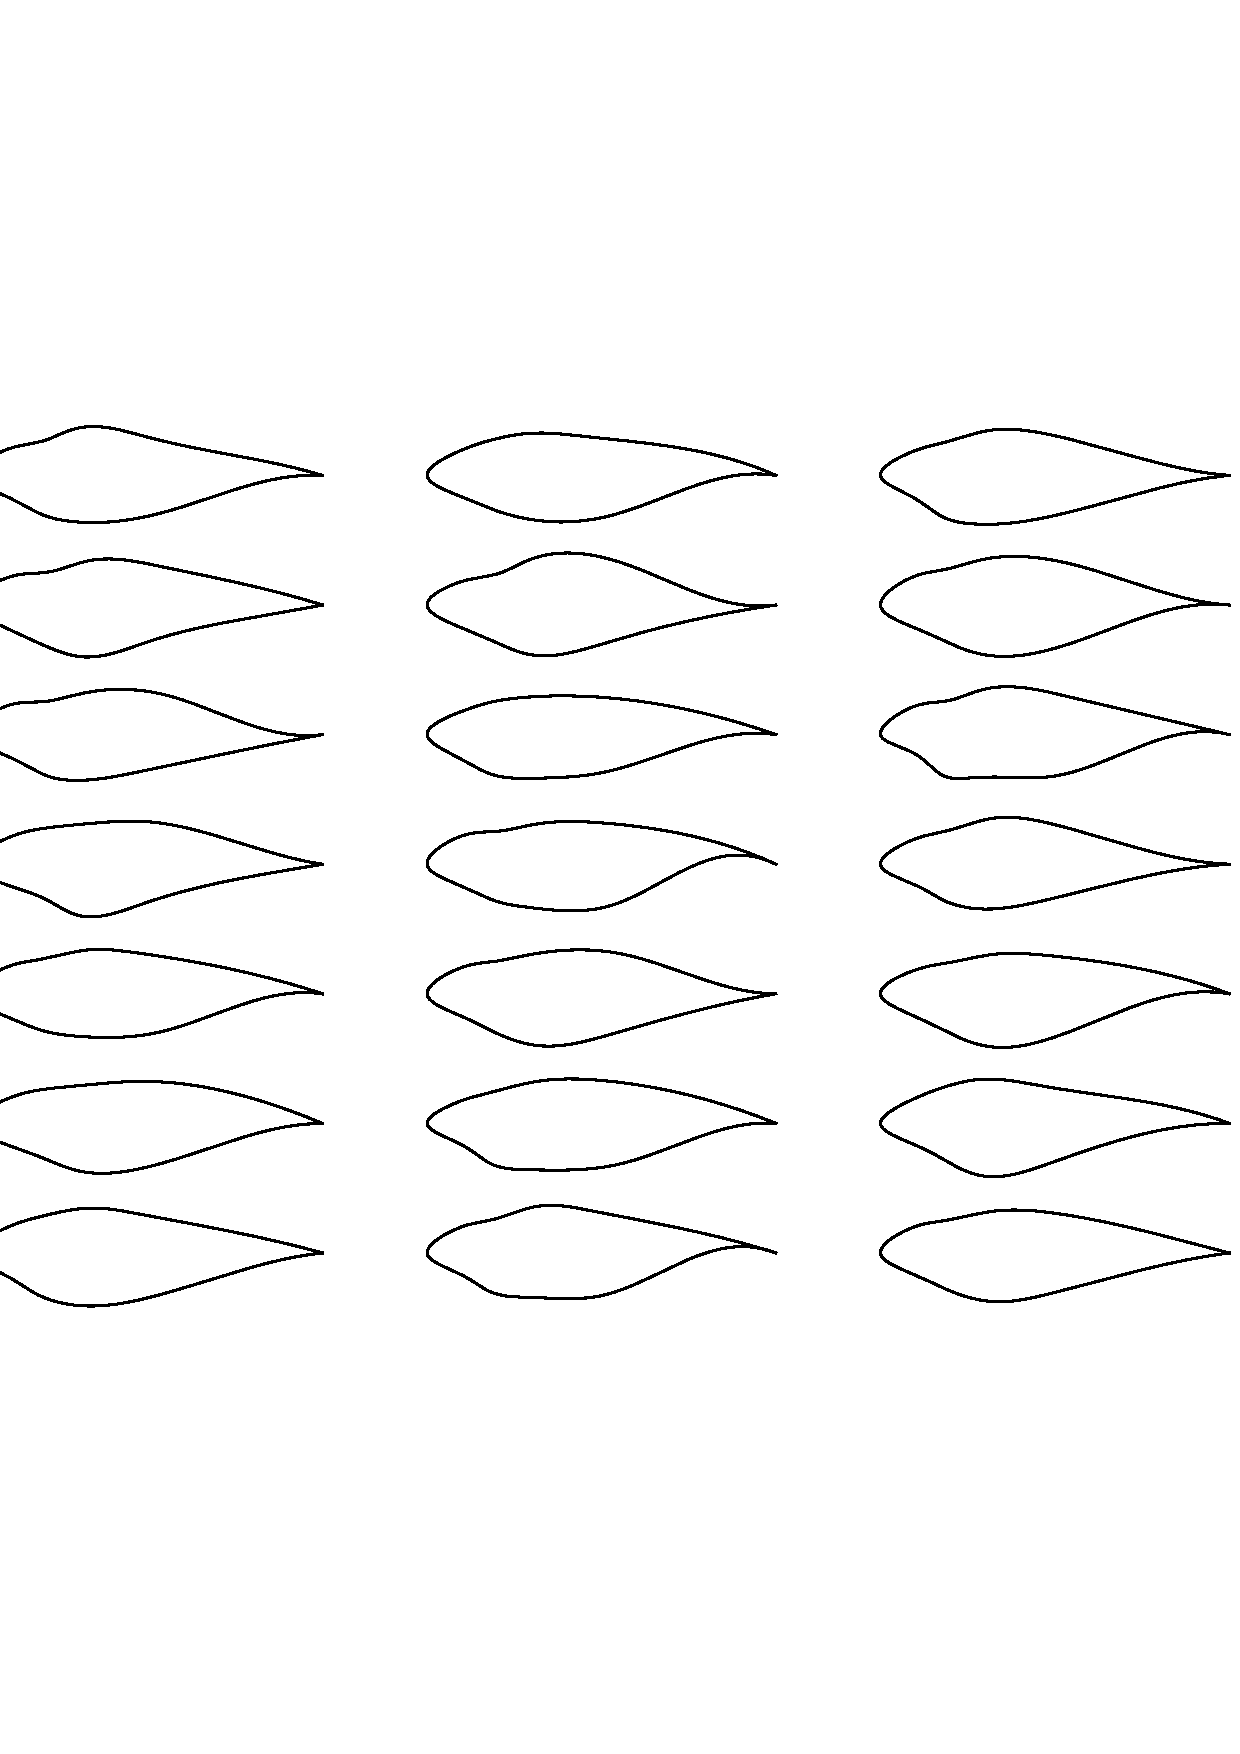
\includegraphics[width=1\textwidth]{initpop}
  \caption{Initial populations rot-vingprofiler skapad genom variationer på S809 med 10 \% slumpfaktor i varje punkt.}
  \label{initpop}
\end{figure}

\pagebreak

\subsection{Implementering av den genetiska algoritmen}

Biblioteket \textsc{Deap} till programmeringsspråket Python har använts med parametrar enligt \tref{GAparametrar} och algoritmen \lstinline[breaklines=true]!eaSimple!. Denna valdes eftersom det är en enkel implementation och trots litteraturstudien visat att mer avancerade algoritmer kan ge resultat till lägre beräkningskostnad. 


\bigskip
\begin{table}[!htb]
\small
  \centering
  
    \begin{tabular}{ll}
    
    \toprule
    Parameter & Värde \\
    \midrule
    Mutationssannolikhet för en individ ($MUT_{pb}) $ & 10 \%  \\
    Mutationssannolikhet för arvsmassans individuella element ($IND_{pb}) $ & 10 \%  \\
    Standardavvikelse för den gaussiska slumpfaktorn ($\sigma$) & 2 \% \\
    Sannolikhet att avkomma skapas genom korsning ($CX_{pb}$) & 50 \% \\
    Antal generationer innan avslut  ($N_G$)  & 10 000 st \\
    Populationsstorlek & 600 st \\
    \bottomrule
    \end{tabular}
  \caption{Parametrar för den genetiska algoritmen}
  \label{GAparametrar}
\end{table}

\bigskip
\vbox{%

 \lstinline[breaklines=true]!eaSimple! utsätter först en initial population för \emph{fitness-funktionen}. Efter detta påbörjas en generationsloop i vilken:
 
 
\begin{enumerate}
  \item Populationens individer utsätts för korsning med $CX_{pb}$ procents sannolikhet.
  \item De kvarvarande individerna utsätts för mutation enligt $MUT_{pb}$ procents sannolikhet där
  
  
  \begin{enumerate}
    \item arvsmassans element muteras med $IND_{pb}$ procents sannolikhet
    \item med en gaussisk avvikelse där standardavvikelsen är $\sigma$
  \end{enumerate}
  
  \item Alla individer skapade enligt ovan samt de kvarvarande orörda individerna överförs till nästa generation och processen återupprepas tills $N_G$ antal generationer passerat eller att användaren avslutar processen.
\end{enumerate}

} % end vbox

Förfarandet för  \lstinline[breaklines=true]!eaSimple! som i korthet här beskrivits återges mer utförligt i kapitel 7 av \citet{eaSimple}.




\pagebreak

\subsection{Fitnessfunktion}
\label{fitnessfunk}

\textsc{Bem}-metoden beskriven i \ref{siteoptBEM} ger alltså, givet en uppsättning vindhastigheter - en effektkurva. Denna kan med sannolikheterna för respektive vindhastigheter $h(U)$ (se \ref{vindhastighetsprofiler}) ge en genomsnittseffekt $\overline{P}$. Detta görs genom att sannolikhetsfördelningen $f_w$ aproximeras med vindhastighetshistogrammet $h(U)$ enligt

\begin{subequations}
\begin{align*}
        \overline{P} &= \int_{U_{in}}^{U_{ut}}f_w(U)P(U)dU \\
        &\approx  \sum_{U_{in}}^{U_{ut}} h(U)P(U)
\end{align*}
\end{subequations}

$\overline{P}$ ger nu approximativt hur pass bra ett vindkraftverk är för platsen som vidhistogrammet $h(U)$ beskriver eftersom summan av $h(U) = 1$.

%% ----------------------------------------------------------------
%% Results.tex
%% ---------------------------------------------------------------- 
\chapter{Resultat} \label{Chapter:resultat}

\section{Referensfall för verifiering av SiteOpt}

\label{mattstocksfall}




Amerikanska \emph{National Renewable Energy Laboratory} (NREL) har utfört flera väldokumenterade experiment på vindkraftverk där all data tillgängliggjorts \citep{UAE}. Av dessa har det som benämnts \emph{Unsteady Aerodynamics Experiment Phase III} (vidare kallat UAE III) valts som ett referensfall. Ytterligare ett referensfall från universitetet i Waterloo, Canada beskrivet i \citet{Canada} har även valts ut (vidare kallat Waterloo). Båda valdes eftersom de med enkelhet kunde reproduceras med studiens modell (SiteOpt).

I \tref{UAEIIoIII} resenteras UAE IIIs och Waterloos specifikationer tillsammans med Reynoldstalen $Re_{min}$ och $Re_{max}$ som utvärderingen gjorts mellan i $N_{Re}$ st steg.





\pagebreak

\begin{savenotes}

\begin{table}[!h]

\centering
  
    
    \begin{tabular}{lrr}
    
    \toprule
    & \multicolumn{2}{c}{Experiment} \\
    \cmidrule(r){2-3}
        & Waterloo & UAE III \\
    \midrule
    Antal blad (st)   & 3  & 3 \\
    Rotordiameter (m)  & 3.3 & 10.046      \\
    Hubradie (m) & 0.144  & 0.72      \\
    Rotationshastighet (RPM) & 200 & 71.63      \\
    Inkopplingshastighet (m/s) & 3.6      & 5       \\
    Märkeffekt (kW) & - & 19.8 \\
    Korda (m) & Se \tref{twist} & Konstant 0.4572 \\
    Pitch ($\theta_p$) ($^{\circ}$) & 0 & 3 \\
    Toppvingprofil & S833\footnote{Studiens modell har ej tagit hänsyn till att rotorbladets sista 5 \% egentligen ska bestå av S834} & S809 \\
    Mellanvingprofil & S835\footnote{Denna placeras vid rotorbladets mitt trots att den är specificerad till 40 \% av rotorbladet.} & S809 \\
    Rotvingprofil & S835 & S809 \\
    \emph{Twist} ($^{\circ}$) & Se \tref{twist} & Se \tref{twist} \\
    Reynoldsupplösning $N_{Re}$ (st) & 12 & 12 \\
    $Re_{min}\times10^5$ & 1 & 5 \\
    $Re_{max}\times10^5$ & 11 & 60 \\
    \bottomrule
    \end{tabular}
  \caption{Specifikationer för referensfallen \emph{Waterloo och UAE III}}
  \label{UAEIIoIII}
  
\bigskip\bigskip
\end{table}
\end{savenotes}
\pagebreak


\bigskip\bigskip\bigskip\bigskip\bigskip\bigskip\bigskip\bigskip\bigskip
\begin{table}[!h]

  \centering
  
  
\begin{tabular}{lrrrr}
\toprule
      & \multicolumn{2}{c}{UAE III} & \multicolumn{2}{c}{Waterloo} \\ \cline{2-5} 
Normerad radie (r/R) & Twist ($^{\circ}$)        & Korda (m)        & Twist ($^{\circ}$)         & Korda (m)         \\
    \midrule
    0.14   & 44.67 & 0.45 & 18.99 & 0.30 \\
    0.18 & 39.39  & 0.45  & 19.01 & 0.29\\
    0.23 & 32.29  & 0.45  & 19.00 & 0.28\\
    0.28 & 26.56  & 0.45 & 18.02 & 0.26 \\
    0.33 & 21.95  & 0.45  & 16.30 & 0.25\\
    0.38 & 18.19  & 0.45 & 14.94 & 0.24 \\
    0.43 & 15.10  & 0.45 & 13.42 & 0.23 \\
    0.48 & 12.51  & 0.45 & 11.83 & 0.22 \\
    0.53 & 10.35  & 0.45 & 10.03 & 0.20 \\
    0.58 & 8.50  & 0.45 & 8.45 & 0.19 \\
    0.64 & 6.91  & 0.45 & 6.91 & 0.18 \\
    0.67 & 5.52  & 0.45 & 6.54 & 0.17 \\
    0.73 & 4.32  & 0.45 & 5.76 & 0.16 \\
    0.77 & 3.25  & 0.45 & 5.28 & 0.15 \\
    0.85 & 2.30  & 0.45 & 4.24 & 0.13 \\
    0.89 & 1.45  & 0.45 & 3.31 & 0.12 \\
    0.93 & 0.69  & 0.45 & 2.41 & 0.11 \\
    1.00 & 0.00  & 0.45 & 2.01 & 0.10 \\
\bottomrule
\end{tabular}


  \caption{Twist- och kordadistribution längs rotorbladet i UAE III \citep{UAE} och Waterloo \citep{Canada}}
  \label{twist}
\end{table}

\pagebreak

UAE III och Waterloo har utvärderats i studiens modell (SiteOpt) där resultatet i \fref{UAEIII} och \fref{Canada} erhållits. Här syns även  experimentellt uppmätta data för experimenten. 

SiteOpt visar överensstämmande resultat vid låga vindhastigheter. Men vid lite högre vindhastigheter misslyckas SiteOpt att förutsäga utplaningen av effekt som uppstår. Detta är extra tydligt i Waterlooexperimentet (\fref{Canada}) där vindhastigheter innan 8 m/s har väldigt god överensstämmelse men efter det helt avviker från den experimentella datan.

\begin{figure}[!h]
  \centering
   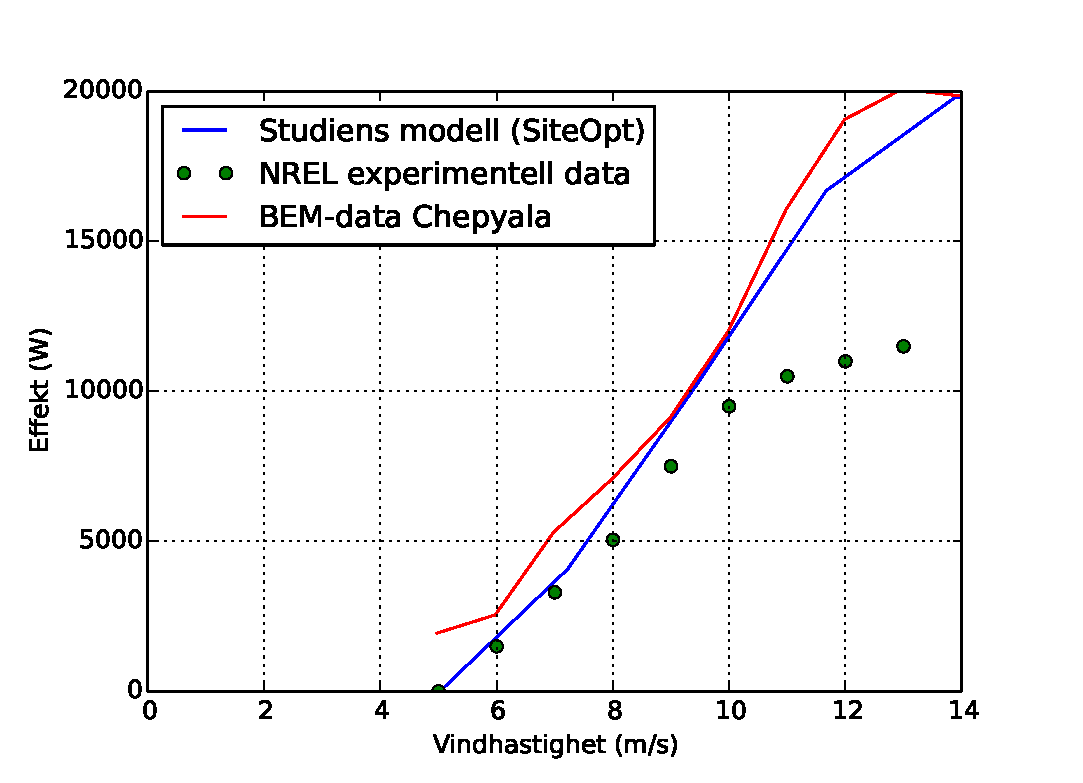
\includegraphics[width=0.7\textwidth]{UAEIII}
  \caption{Resultat av UAE III utvärderat i SiteOpt vid olika vindhastigheter samt experimentell data från \citet{UAEIIIdata}.}
  \label{UAEIII}
\end{figure}

\begin{figure}[!h]
  \centering
  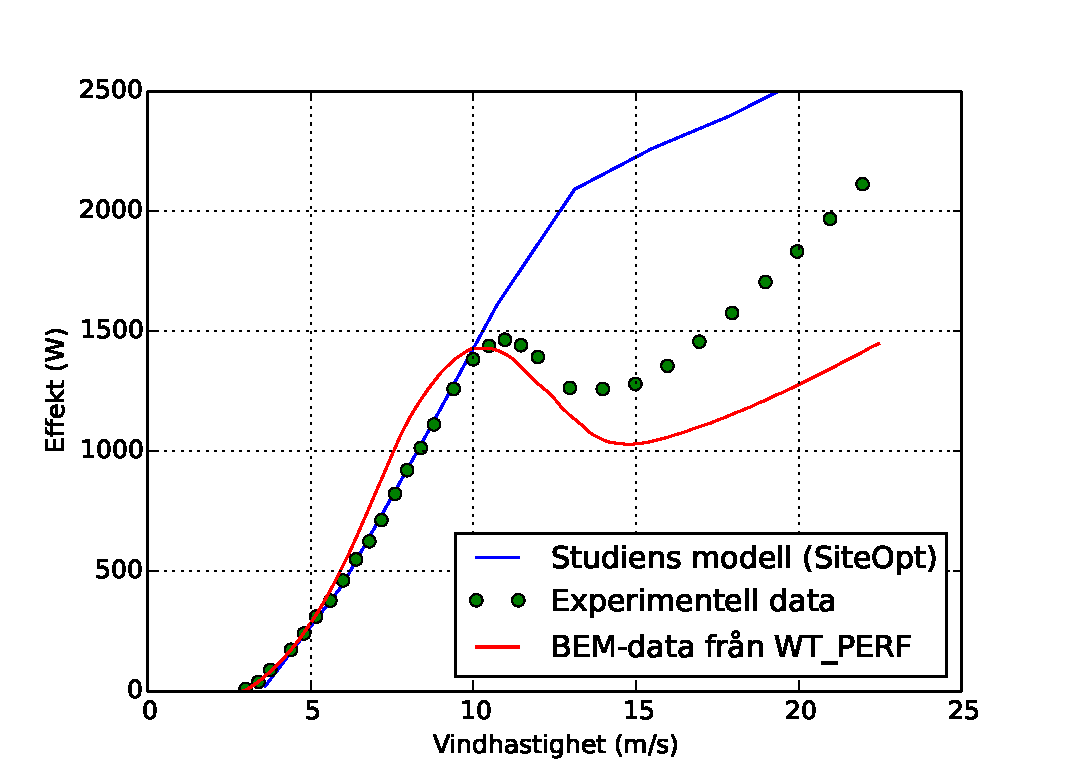
\includegraphics[width=0.7\textwidth]{Canada}
  \caption{Resultat av vindkraftverket beskrivet i \citet{Canada} (Waterloo) utvärderat i SiteOpt vid olika vindhastigheter samt experimentell data.}
  \label{Canada}
\end{figure}

\fref{Canada} visar även Waterlooexperimentet utvärderat i den vanligt förkommande \textsc{Bem}-programvaran \textsc{wt\_perf} av \citet{Canada}. Detta visar att \textsc{Bem} bör kunna förutsäga höga vindhastigheter betydligt bättre än de som studiens modell (SiteOpt) producerar. Även om SiteOpt (åtminstone i detta fall) visar bättre överensstämmelse vid låga vindhastigheter än \textsc{wt\_perf}.

I \fref{UAEIII} visas även data genererat med \textsc{Bem} från masteruppsatsen \citet{CST} (utmarkerat med rött) vilken visar samma avvikande beteende som studiens modell. Detta tyder på att \citet{CST} gjort samma eller liknande misstag som i denna studie. Stora ansträngningar har gjorts för att utröna orsaken till detta och en diskussion om möjliga orsaker återfinns i \ref{slutsatser}.

För fullständig loggdata av SiteOpts simulering av UAE III se Appendix B. Här framkommer att vindhastigheter över 8 m/s även medför högre angreppsvinklar.





\pagebreak
\section{Optimering av UAE III}

UAE III har använts som utgångspunkt för studiens optimering. I \tref{optimeringsspec} syns hur samma specifikationer som i UAE III använts. Nu har korda-, twistdistribution och vingprofil tillåtits variera (det vill säga agerat designvariabler) för att nå resultaten som presenteras här. $Re$ har satts till att endast utvärderas vid $20\times10^5$ för att spara tid. SiteOpts möjlighet att ha olika vingprofiler längs radien har inte använts av samma skäl.

\bigskip
\begin{table}[!htb]
  \centering
  
    \begin{tabular}{lrr}
    \toprule
    %& \multicolumn{2}{c}{Experiment} \\
    %\cmidrule(r){2-3}
        & Utgångsvärde & Fixerat eller variabelt \\
    \midrule
    Antal blad (st)  & 3  & Fixerat \\
    Rotordiameter (m) &  10.046   & Fixerat    \\
    Hubradie (m) &  0.72  & Fixerat     \\
    Tornhöjd (m)       & 17.03     & Fixerat      \\
    Rotationshastighet (RPM) & 71.63 & Fixerat     \\
    Inkopplingshastighet (m/s) & 5 & Fixerat      \\
    Märkeffekt (kW) & 19.8 & Fixerat \\
    Korda (m) & 0.4572 & Variabel längs radien \\
    Pitch ($\theta_p$) ($^{\circ}$) & 3 & Fixerat \\
    Vingprofil & S809 & Variabel, dock samma längs radien  \\
    $Re\times10^5$ & 20 & Fixerat \\
    Vindhistogram & Se \ref{vindhastighetsprofiler} & Fixerat \\

    \emph{Twist} ($^{\circ}$) & Se tabell \ref{twist} & Variabelt längs radien
    \bottomrule
    \end{tabular}
  \caption{Specifikationer för optimeringen som görs med utgångspunkt i UAE III}
  \label{optimeringsspec}
\end{table}

\begin{figure}[!htb]
  \centering
  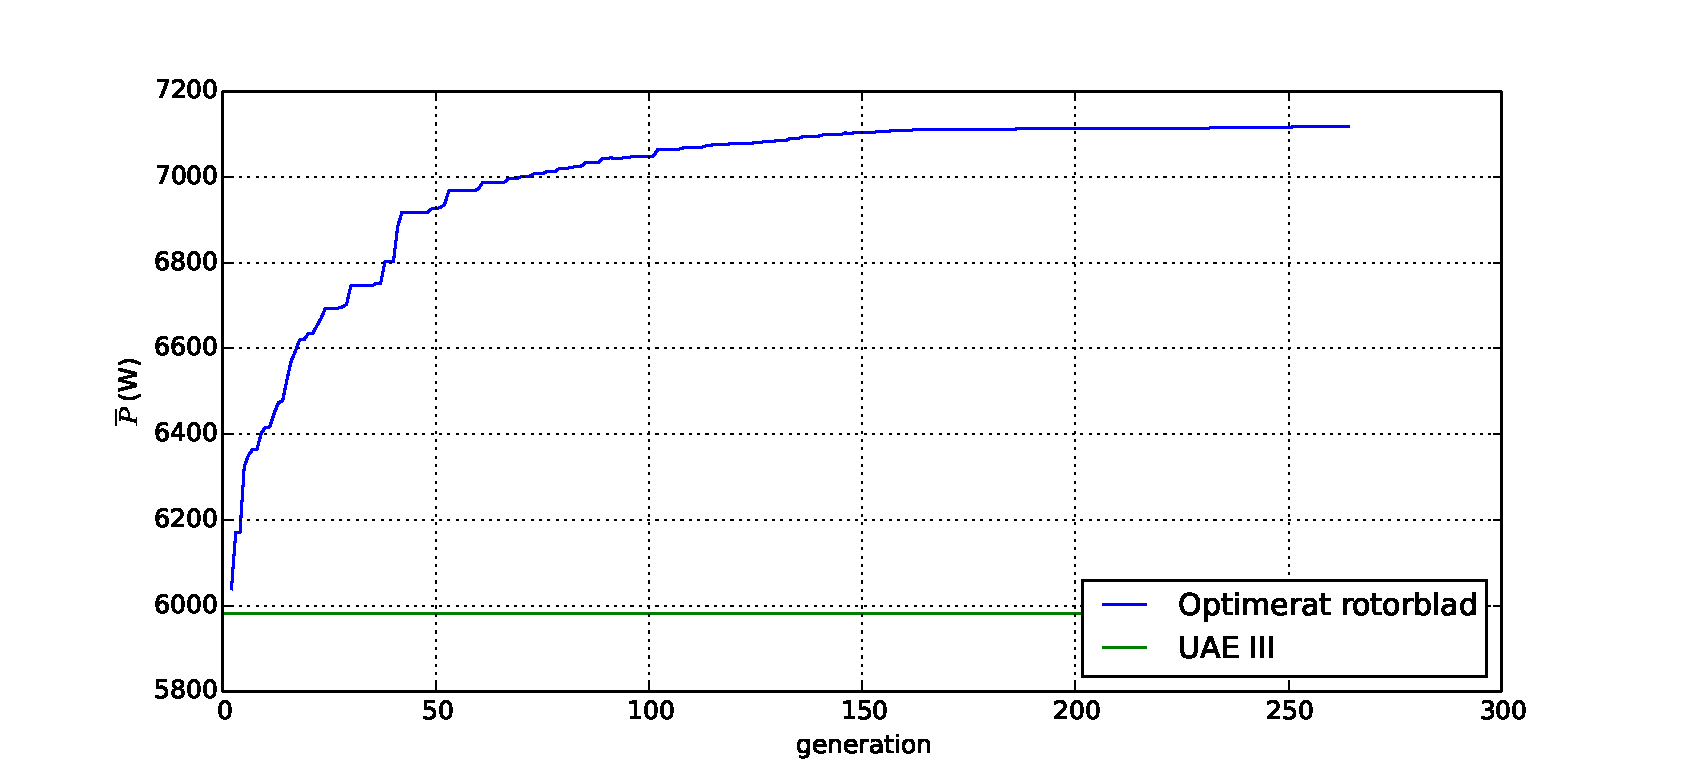
\includegraphics[width=1\textwidth]{GAutveckling}
  \caption{Figur illustrerande hur genomsnittseffekten $\overline{P}$ av den bästa individen i varje generation utvecklas med ytterligare generationer i den genetiska algoritmen.}
  \label{GAutveckling}
\end{figure}


\bigskip
\begin{table}[!htb]
  \centering
  
    \begin{tabular}{ll}
    \toprule
    Hårdvara & Specifikation \\
    \midrule
    Processor  & 2.8GHz quad-core Intel Core i7 \\
    Minne & 8GB (2 x 4GB) 1333MHz DDR3
    \bottomrule
    \end{tabular}
  \caption{Specifikationer för använd hårdvara}
  \label{datorspec}
\end{table}

Efter 265 generationer har ett c:a 15 \% bättre resultat än UAE III erhållits vilket syns i \fref{GAutveckling}. Använd hårdvara syns i \tref{datorspec} och med denna tog optimeringen ungefär 7 dagar vilket betyder att en genomsnittlig generation tog c:a 38 minuter. I \fref{GAutveckling} syns även att konvergens infinner sig redan vid ungefär 150 generationer varpå väldigt små förbättringar uppnås. Notera att det är genomsnittseffekten $\overline{P}$ uträknat enligt förfarandet i \ref{fitnessfunk} med vinddata från St. Lawrence, Canada. Med modellens svaga förmåga att förutsäga effekt vid höga vindhastigheter i åtanke, kan det vara intressant att notera att 81 \% av vinddatan befinner sig innan 10 m/s. Det är även endast den bästa individen i varje generation som presenteras i \fref{GAutveckling}.

\begin{figure}[!htb]
  \centering
  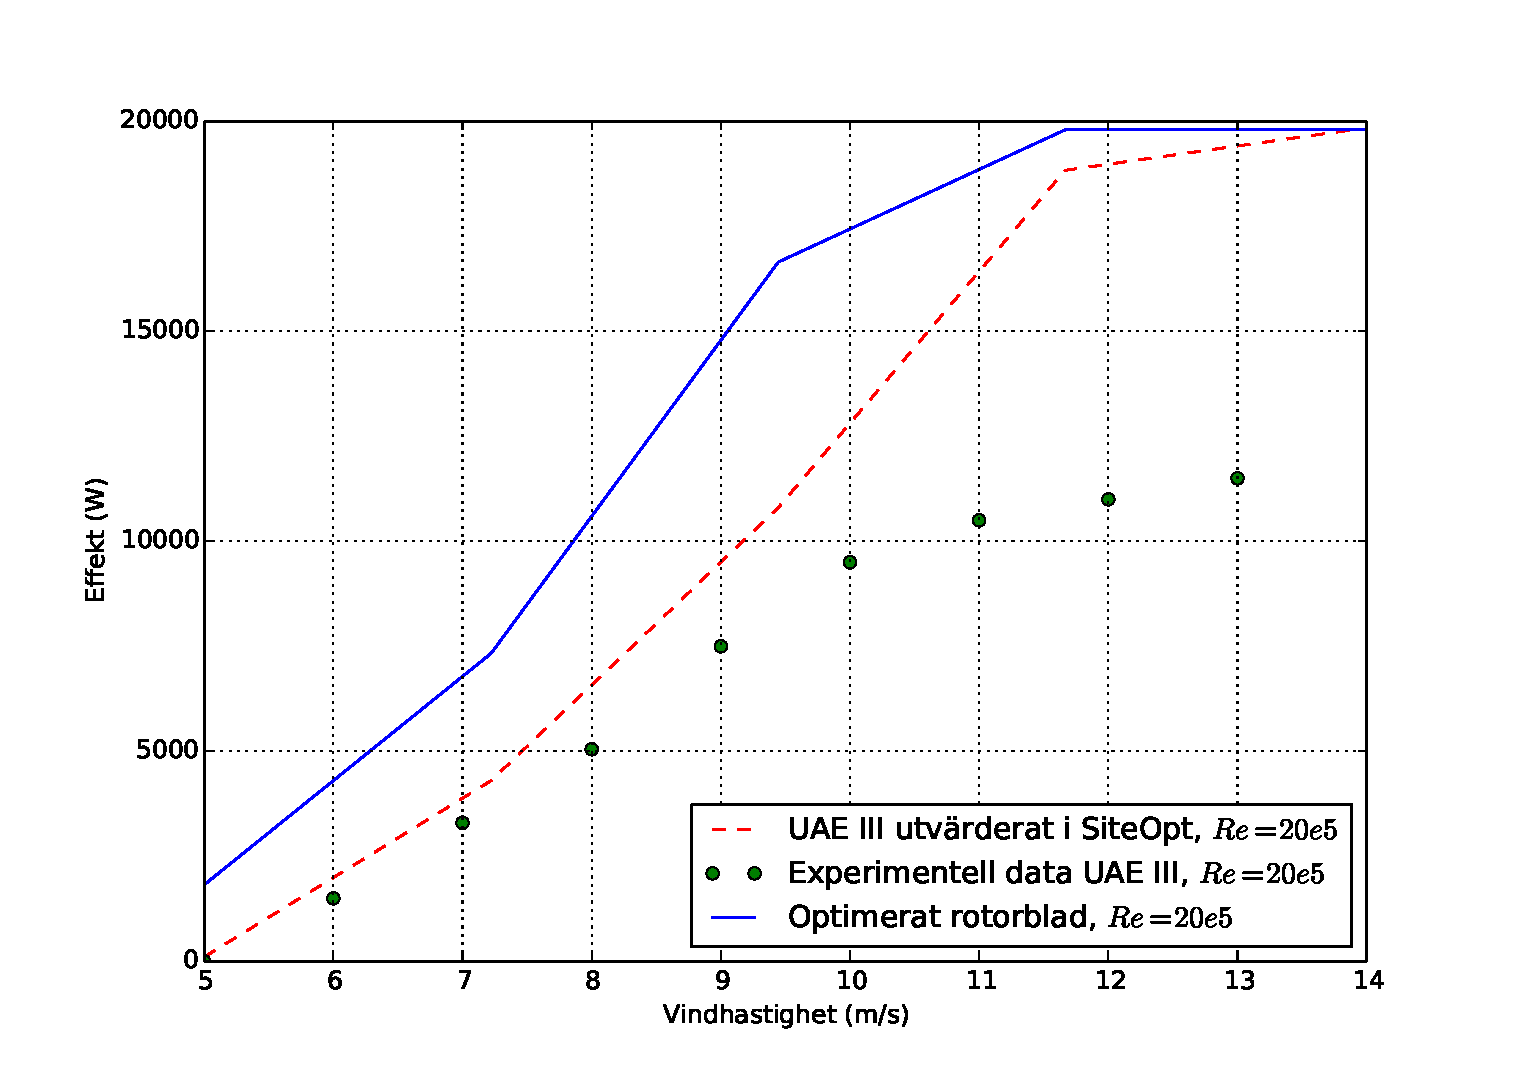
\includegraphics[width=1\textwidth]{powercurvecompare}
  \caption{Effektkurvor för referensfallet UAE III och det optimerade rotorbladet.}
  \label{powercurvecompare}
\end{figure}

Effektkurvan för det rotorbladet som optimeringen tagit fram ses i \fref{powercurvecompare}. Notera att SiteOpts utvärderade effektkurva avviker lite från den i \ref{mattstocksfall} eftersom denna endast är utvärderad vid $Re = 20\times10^5$.

Vingprofilen som optimeringen tagit fram visas i \fref{AFjamforelse} tillsammans med utgångspunkten S809 för jämförelse och är alltså samma för hela rotorbladet. 

\begin{figure}[!h]
  \centering
  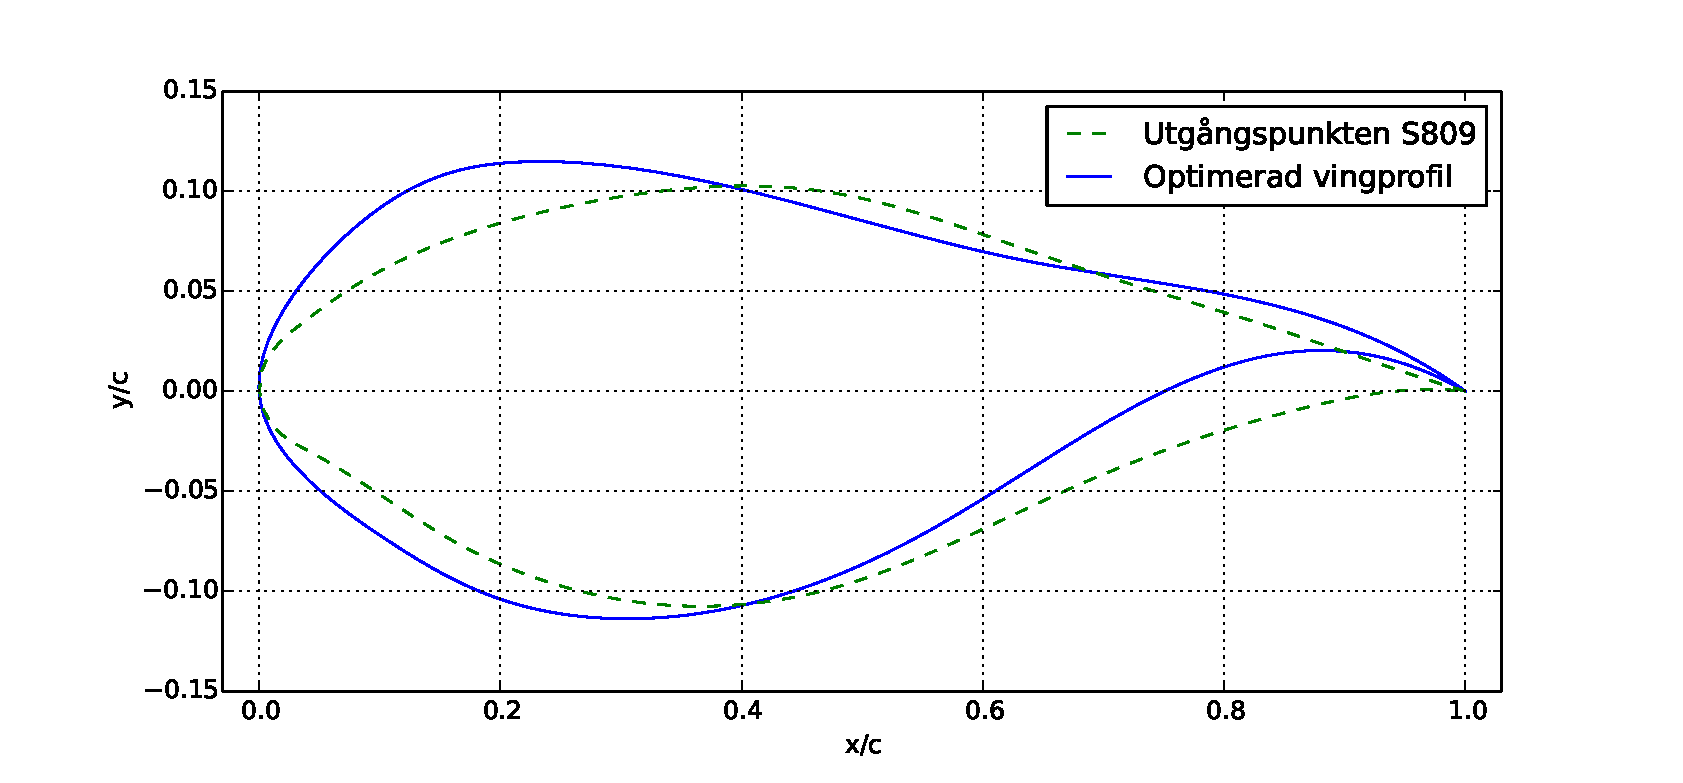
\includegraphics[width=1\textwidth]{AFjamforelse}
  \caption{Den optimerade vingprofilen jämfört med ursprungsprofilen S809.}
  \label{AFjamforelse}
\end{figure}

I \fref{kordatwistjamforelse} syns hur korda- och twistdistribution skiljer sig från utgångspunkten UAE III. 

\begin{figure}[!h]
  \centering
  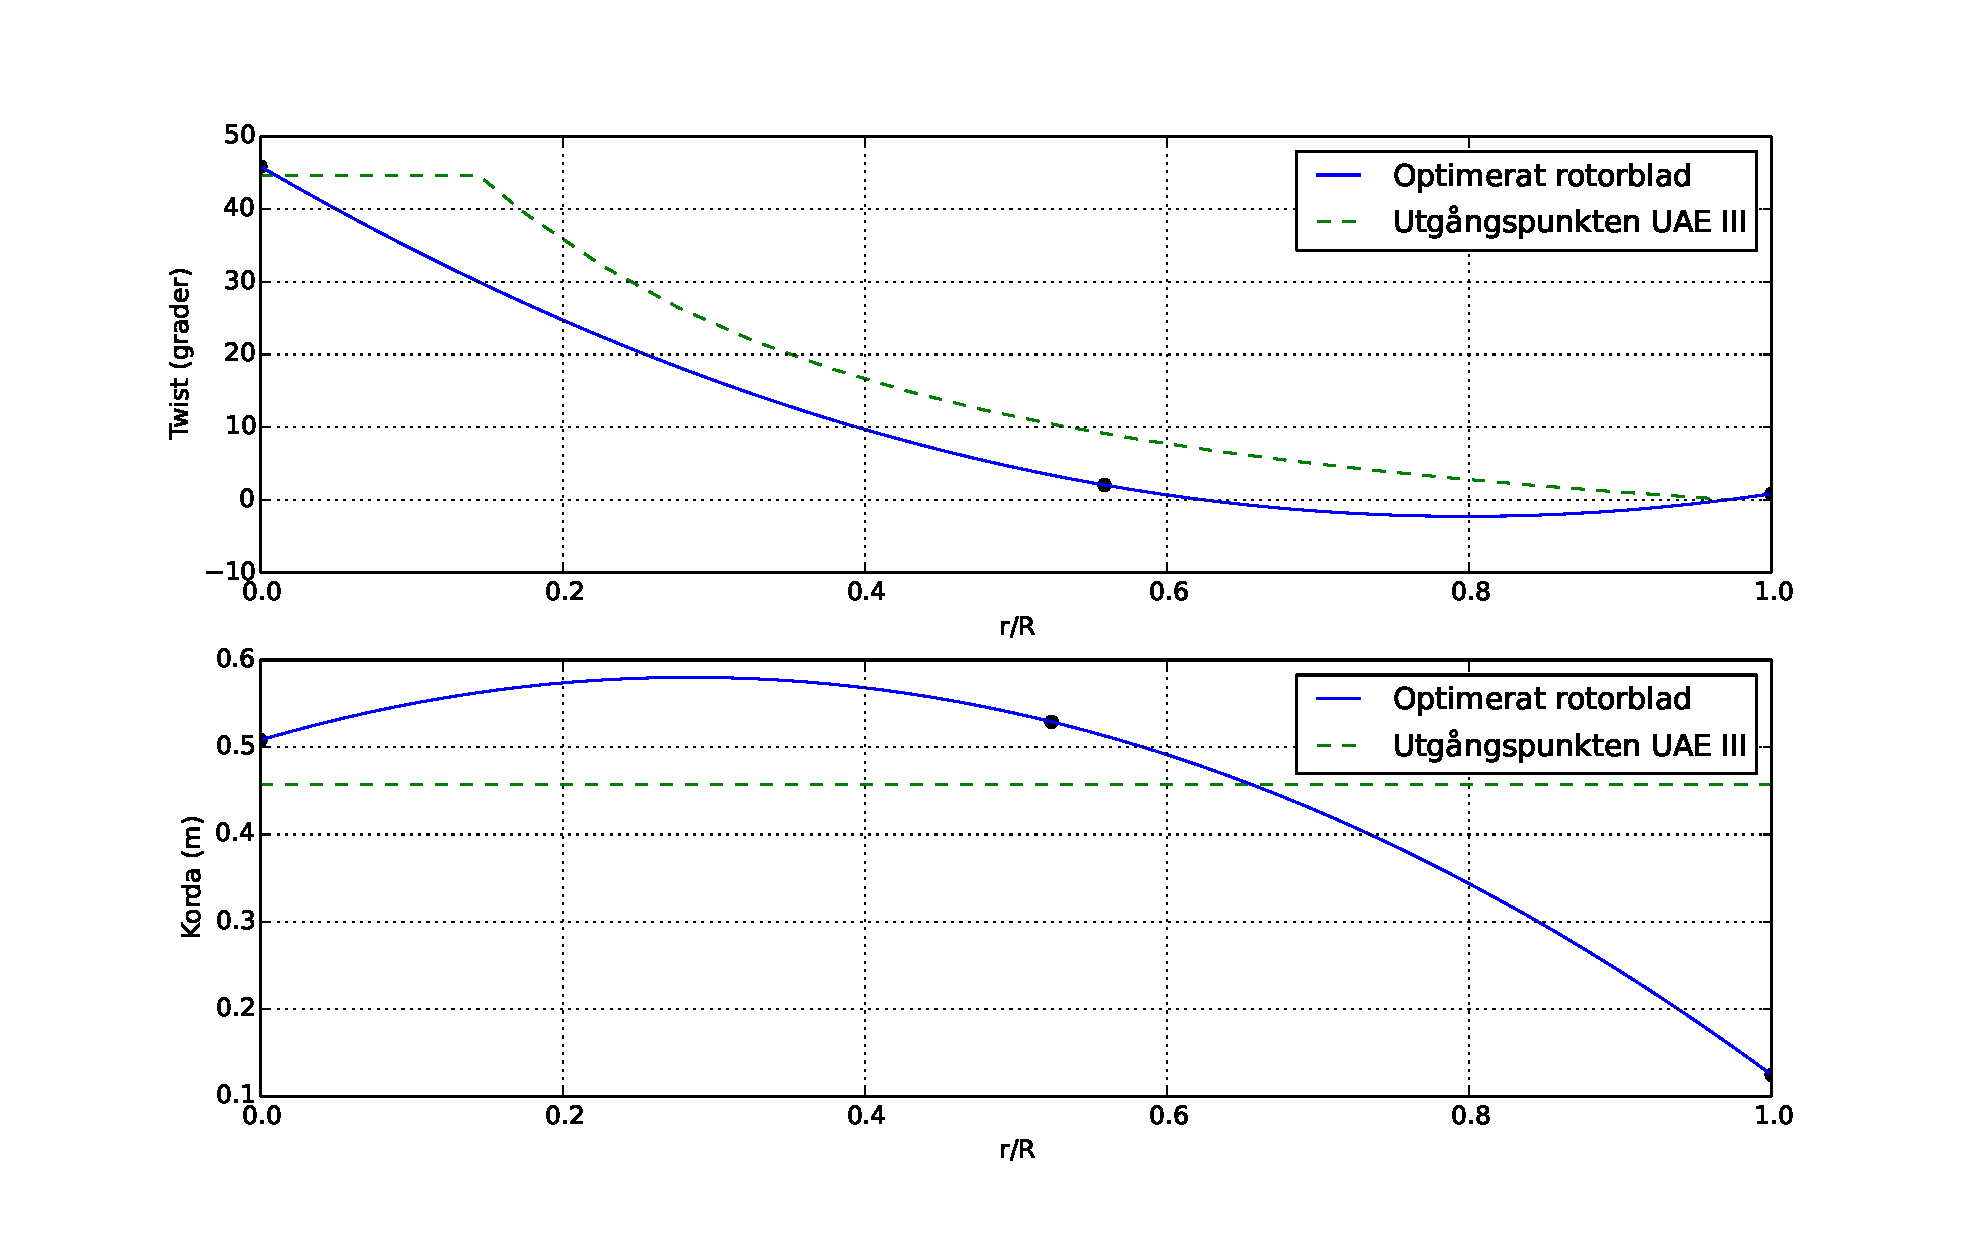
\includegraphics[width=1\textwidth]{kordatwistjamforelse}
  \caption{Det optimerade rotorbladets korda- och twistdistribution jämfört med utgångspunkten UAE III.}
  \label{kordatwistjamforelse}
\end{figure}

I \fref{Cljamforelse} och \fref{Cdjamforelse} presenteras lyft- och motståndskoefficientdata för den optimerade vingprofilen i jämförelse med datan \textsc{Xfoil} ger för S809. Även experimentell data för S809 har inhämtats från \citet{s809re20}. Detta ger en indikation på hur mycket \textsc{Xfoil} överskattar lyft- och motståndskoefficienter vid högre $\alpha$ vilket framkom i litteraturstudien. Detta  bör tas i beaktande när den optimerade vingprofilens data studeras.

\begin{figure}[!htb]
  \centering
  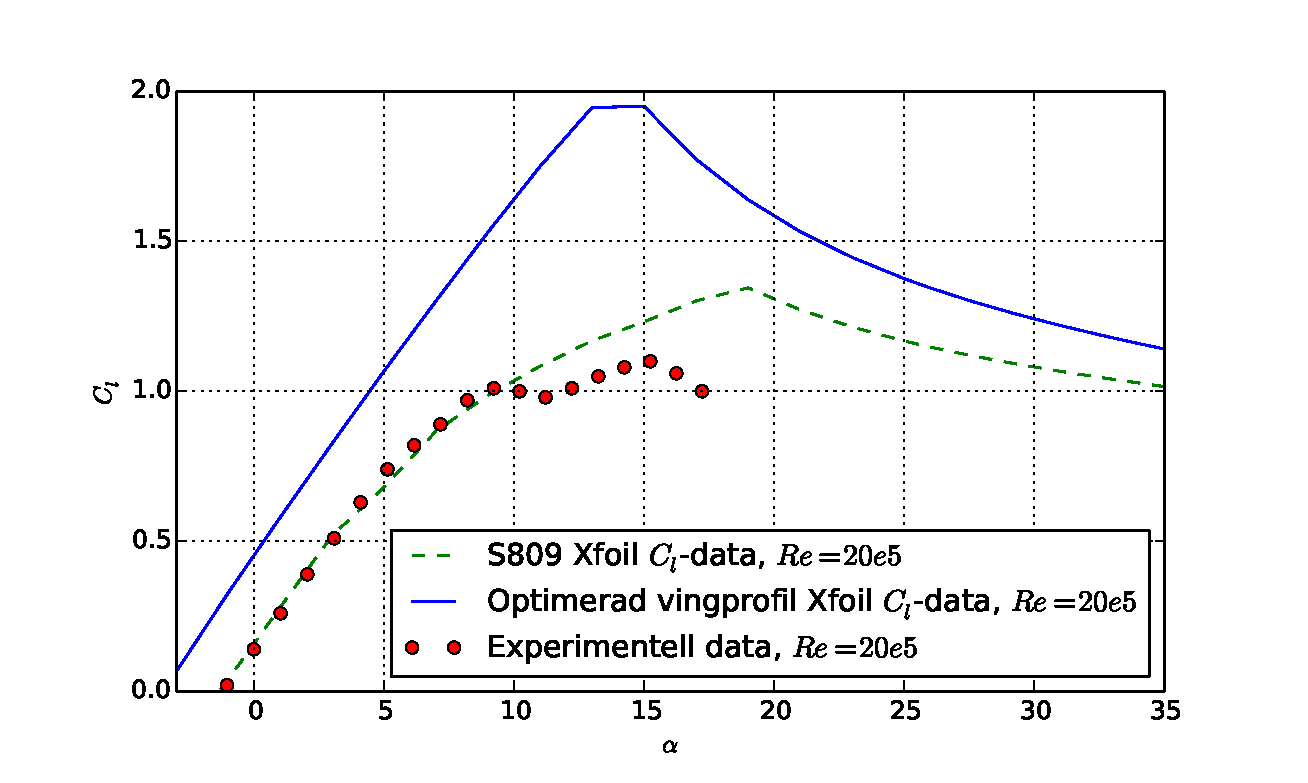
\includegraphics[width=1\textwidth]{Cljamforelse}
  \caption{Lyftkoefficient för den optimerade vingprofilen och utgångspunkten S809 utvärderat i \textsc{Xfoil} samt experimentell data för S809 från \citet{s809re20}.}
  \label{Cljamforelse}
\end{figure}

\begin{figure}[!htb]
  \centering
  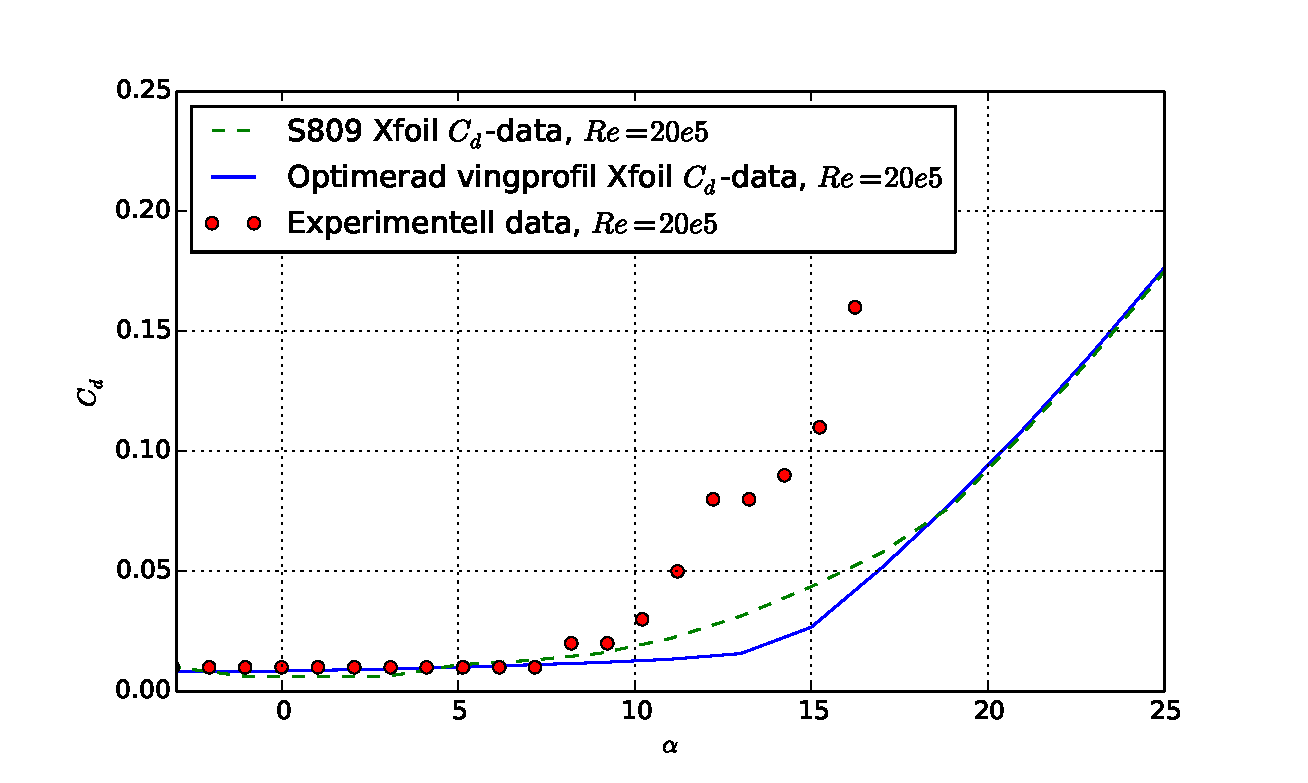
\includegraphics[width=1\textwidth]{Cdjamforelse}
  \caption{Motståndskoefficient för den optimerade vingprofilen och utgångspunkten S809 utvärderat i \textsc{Xfoil}.}
  \label{Cdjamforelse}
\end{figure}


%% ----------------------------------------------------------------
%% Discussion.tex
%% ---------------------------------------------------------------- 
\chapter{Diskussion} \label{Chapter:diskussion}

\section{Sammanfattning}

I studien har en metodologi utvecklats för att kunna optimera ett vindkraftverks rotorblad för ett användarvalt vindhastighetsförhållande. Givet vindhastighetsdata och via den för studien utvecklade programvaran, där \textsc{Bem}-teori implementerats - kan en genomsnittseffekt erhållas. Detta används som målfunktion i en optimeringsalgoritm av slaget genetiska algoritmer, vilket producerar ett optimerat rotorblad. 

Följande punkter sammanfattar studiens metodologi:

\begin{description}
  \item[Vingprofilsrepresentation] Vingprofiler har representerats genom att 12 diskreta punkter sammanbundits av kubiska B-splines. Detta har visats vara en avvägning mellan mycket detaljer och hög beräkningstid samt få detaljer och inskränkt designrymd.
  \item[Rotorbladssrepresentation] Ett vindkraftverks rotorblad har beskrivits med tre vingprofiler (rot, mellan och topp) där mellanliggande vingprofiler interpoleras fram. Detta resulterar i 12 radiella bladelement. Vingprofilerna sattes till en och samma i alla positioner vid optimeringen för att påskynda resultaten. 
  

  \item[Vingprofilers aerodynamiska egenskaper] Programvaran \textsc{Xfoil} har använts för att erhålla lyft- och motståndskoefficienter ($C_l$ och $C_d$). Givet en vingprofil, attackvinkel $\alpha$ och Reynolds tal $Re$ kunde detta erhållas till relativt låg beräkningskostnad. Möjlighet att utvärdera för lyft- och motståndskoefficient vid flera $Re$ gavs men för att åter igen spara tid, utvärderades dessa endast vid $Re = 20\times10^5$.
  
Eftersom \textsc{Xfoil} inte kan ge resultat långt efter stallvinkeln $\alpha_{stall}$ görs en extrapolering med viternaekvationerna, det antas även att vingprofilen beter sig som en platta vid extremt höga och låga attackvinklar. Denna extrapolering ger då lyft- och motståndskoefficienter för hela spannet $\pm 180^{\circ}$.
  
  
  
  \item[Vindkraftverks effekt] \textsc{Bem}-metoden ger ett vindkraftverks uppskattade effekt vid olika vindhastigheter. Genom att para denna data med vindhastighetsdata för ett specifikt vindförhållande har en genomsnittseffekt $\overline{P}$ kunnat tas fram. Detta har sedan använts som målunktion i optimeringsprocessen. I studien användes godtyckligt vinddata för St. Lawrence i Kanada.
  
  \item[Optimering] En genetisk algoritm har använts via Pythonbiblioteket \textsc{Deap} som genom att imitera evolutionen itererar fram vindkraftverk med högre genomsnittseffekt.
  
\end{description}

Följande resultat kunde sedan presenteras:

\begin{description}

\item[Utvärdering av modell] Genom att utgå från ett akademiskt vindkraftverk (Unsteady Aerodynamics Experiment Phase III, UAE III) där vingprofilen S809 används längs hela rotorbladet har metodologins modell utvärderats. Här visas att den för studien utvecklade modellen (SiteOpt) dramatiskt överskattar ett vindkraftverks effekt för vindhastigheter över 8 m/s, men ger god överensstämmelse innan 8 m/s.

\item[Resultat av optimering] En optimering av slaget genetisk algoritm har sedan utförts. Detta har gjorts med hänsyn till den inmatade vinddatan. Denna visas till 81 \% ligga innan 10 m/s där modellen visar acceptabel överensstämmelse med vindtunneldata. Detta resulterade i en ny vingprofil  som ses i \fref{AFjamforelse} samt en \emph{twist}- och kordadistribution. Detta resultat har enligt modellen ett ökat genomsnittseffektuttag över ett år på 15 \% jämfört med utgångspunkten UAE III.

\end{description}

%Resultaten visade att 15 \% ökat effektuttag jämfört med utgångspunkten UAE III teoretiskt kunde erhållas


\section{Slutsatser}
\label{slutsatser}

Följande slutsatser kan dras från resultaten, och presenteras här med viktigast slutsats först och sedan i fallande ordning.

\begin{enumerate}

    \item Studiens modell (SiteOpt) visar en ökning av genomsnittseffekten $\overline{P}$ på 15 \% mot referensfallet UAE III efter att optimeringen genomförts. Detta betyder att med den föreslagna optimerade vingprofilen (\fref{AFjamforelse}) och korda/\emph{twist}-distribution (\fref{kordatwistjamforelse}) kan teoretiskt sätt 15 \% mer elektricitet tas ut årligen än utgångspunkten. Detta givet att modellen är en bra representation av verkligheten. 
      
    \item Studiens modell har dessvärre visats vara en dålig representation av verkligheten efter c:a 8 m/s. Varför avvikelsen uppstår har inte kunnat fastställas och en annan programvara med implementering av BEM har visats ha betydligt bättre överensstämmelse efter 8 m/s. Samma avvikelse har dock hittats i en annan studentuppsats \citep{CST}. Följande är eventuella förklaringar till avvikelsen:
    
        \begin{enumerate}
        \item I denna studie har ingen hänsyn tagits till hållfasthetsaspekter eller rotorblads böjbarhet utan ett helt stelt rotorblad antas. Vid höga vindhastigheter, beroende på rotorbladets material - kommer en krökning i vindens riktning uppstå. Detta gör sannolikt upphov till radiellt flöde. För att \textsc{Bem} ska vara giltigt, får detta ej förekomma. Att \citet{CST} visar liknande avvikelse vid höga vindhastigheter tyder på att en ofullständig modell även använts där. \citet{CST} har likt denna studien inte tagit hänsyn till böjbara rotorblad. Därför är detta att anse som den mest rimliga förklaringen till avvikelsen.


        \item Det har i litteraturstudien framkommit att \textsc{Xfoil} ger dåligt överensstämmande lyft- och motståndskoefficienter efter stallvinkeln $a_{stall}$ samt att \textsc{Xfoil} underskattar motståndskoefficienten $C_d$.  Vid höga vindhastigheter fås även höga angreppsvinklar (se Appendix B). Dessa höga angreppsvinklar har även extrapolerats fram vilket gör att mycket hänger på denna extrapolations korrekthet. Litteraturstudien visade även att \textsc{Bem}s största svaghet är dess lyft- och motståndskoefficienter. Detta låter som en rimlig förklaringsmodell men när dessa felaktigheter försökte kompenseras sågs dessvärre ingen förbättring.
        

        \item Det är även tänkbart att ett implementeringsfel av numeriken är problemet då koden nära följer den föreslagna implementationen i \citet{hansen}. \citet{hansen} behandlar endast ekvationerna och ger ingen ledning i hur olika numeriska misstag ska undvikas. Exempelvis har flera gånger lösningar behövts göras för att undvika att dela med noll under lösningen av \textsc{Bem}ekvationerna. 
        \end{enumerate}
    
    \item Trots modellens avvikelse efter c:a 8 m/s har god överensstämmelse visats vid lägre vindhastigheter. När optimeringen gjordes valdes godtyckligt vindförutsättningarna för St. Lawrence i Kanada. 81 \% av vinden visar sig här vara förlagd innan 10 m/s vilket bör betyda att optimeringen ändå till stor del gjorts med en godtagbar modell. Det går dock inte att utesluta att resultatet påverkats av avvikelsen.
    
    \item Vingprofilen som av optimeringen gav som resultat (\fref{AFjamforelse}) har i bakkant ett tunt parti. Denna tunna ``svans'' kan tänkas vara för skör för att vara realiserbar på ett riktigt rotorblad. Detta är antagligen direkt relaterat till att inga hållfasthetsaspekter tagits med i optimeringen.
    
    \item Det optimerade rotorbladet visas i \fref{powercurvecompare} tillsammans med utgångspunkten UAE III. Här framgår hur avvikelsen efter 8 m/s beter sig. Det är att förvänta att det optimerade rotorbladet om realiserat i verkligheten borde ha en liknande avvikelse och att detta skulle innebära att det ökade effekttutaget är mindre än de 15 \% som presenterades i resultaten.
      
      
    \item Referensfallet UAE III som även används som utgångspunkt i optimeringen gör inga anspråk på att vara ett optimerad vindkraftverk. Detta är ett akademiskt testfall vilket valdes eftersom empirisk data fanns tillgänglig. Därför är sannolikt 15 \% genomsnittlig effektökning mer än vad som kan förväntas ifall optimeringen hade gjorts på ett kommersiellt vindkraftverk.

    \item Referensfallet UAE III har endast en vingprofil över hela rotorbladet och det har även resultatet från optimeringen. Flera vingprofiler längs rotorbladet hade sannolikt gett ytterligare effektökningar och var egentligen önskvärt, men eftersom optimeringen ungefär växer med $\mathcal{O}\left(n\right)$ där $n$ är antalet designvariabler - hade optimeringen då tagit ungefär tre gånger så lång tid vilket det tidsmässigt inte fanns utrymme för.
    


\end{enumerate}



\pagebreak
\section{Rekommendationer för framtida arbete}

Följande rekommendationer för framtida arbete ges här med viktigast först och sedan i fallande ordning.

\begin{enumerate}
    \item Det framtagna optimerade rotorbladets egenskaper skulle kunna verifieras om även en analys gjordes med \textsc{cfd}.

    \item En modell som även tar hänsyn till rotorbladens deformation vid högre vindhastigheter (vanligen kallat fluid structure interactions) skulle öka modellens tillförlitlighet avsevärt.
    
    \item Ytterligare testfall utöver de två i rapporten skulle behövas för att verifiera metoden. 
  
    \item Det skulle även vara extra intressant att undersöka metodens möjligheter att göra förbättringar på kommersiella vindkraftverk. Ett kommersiellt vindkraftverk är att anta redan optimerat. Därför skulle det vara intressant att se hur mycket en platsspecifik optimering skulle kunna öka energiuttaget.
        
 
    \item Optimeringen skulle med fördel utökas till en flermålsoptimering där även hållfasthet togs med. Detta för att vingprofiler och rotorblad med ej realiserbar geometri ska kunna undvikas.
    
    \item Optimeringen gjordes med antagandet att lyft- och motståndskoefficienter kunde antas alltid vara gällande vid $Re \times 10^5 = 20$. Med mer tid skulle SiteOpt kunna utvärdera vid flera Reynolds tal för att undvika detta antagandet men till bekostnad på beräkningstid.
    
    \item Med mer tid skulle även SiteOpt kunna tillåtas optimera fram olika vingprofiler i rotorbladets topp-, mellan- och rotvingprofil.
    
    \item Designvariablerna skulle kunna utökas på flera sätt utan att beräkningskostnaden ökade märkbart:
    \begin{enumerate}
        \item Löptalet $\lambda$ skulle kunna optimeras. Ett vindkraftverk som i detta fallet fungerar med fixerat RPM producerar sällan optimal effekt.
        \item Fler diskreta punkter som definierar \emph{twist}- och kordadistributionen skulle kunna läggas till. Nu används endast tre diskreta punkter vilket är begränsande för rotorblad som eventuellt skulle vara bättre med en mer avancerad geometri.
    \end{enumerate}
    
    %\item SiteOpt skulle genom att optimera på ett kommersiellt vindkraft
    
    \item Metoden beskriven i studien är ett bra exempel på ett problem som skulle kunna lösas snabbare om koden parallelliseras. Då skulle istället flera processorkärnor (eller till och med datorer) kunna användas samtidigt och optimeringen skulle gå väldigt mycket snabbare. 
    
    \item Under uppsatsens slutskede hittades rapporten \emph{A Simple Solution Method for the Blade Element Momentum Equations with Guaranteed Convergence} \citep{Andrew} vilken föreslår ett nytt sätt lösa \textsc{Bem} där garanterad konvergens uppnås. Detta förfarande skulle vara en bättre implementering av \textsc{Bem} än den som använts i denna studie.

    \item $\alpha_{stall}$ uppstår vid olika platser beroende på om angreppsvinkeln ökas eller minskas. Detta fenomen kallat dynamisk stall skulle kunna tas hänsyn med en mer avancerad modell.

\end{enumerate}








\appendix

\backmatter
%\bibliographystyle{ecs}
\bibliographystyle{authordate1}
\bibliography{ECS}
%% ----------------------------------------------------------------
%% AppendixA.tex
%% ---------------------------------------------------------------- 
\chapter{Appendix A: Källkod SiteOpt} \label{Chapter:kallkod}

\newminted{python}{fontsize=\tiny}

\begin{pythoncode}
# http://github.com/maxberggren/SiteOpt

#!/usr/bin/env python
# encoding: utf-8
# python v 2.7
"""
siteOpt.py

Created by Max Berggren 2014-05-10

Licensed under the Apache License, Version 2.0 (the "License");
you may not use this file except in compliance with the License.
You may obtain a copy of the License at

   http://www.apache.org/licenses/LICENSE-2.0

Unless required by applicable law or agreed to in writing, software
distributed under the License is distributed on an "AS IS" BASIS,
WITHOUT WARRANTIES OR CONDITIONS OF ANY KIND, either express or implied.
See the License for the specific language governing permissions and
limitations under the License.

"""

from __future__ import division
import numpy as np
from scipy import interpolate
import subprocess as sp
from StringIO import StringIO
from math import pi, atan, acos, cos, sin, tan, exp, sqrt, radians, degrees
import os

xfoilPath = os.getcwd() + os.path.sep + "Xfoil.app/Contents/Resources/xfoil"


def BlendAirfoils(AF1, AF2, percentAF2):
    delX = AF2.x - AF1.x
    newx = AF1.x + delX*percentAF2
    delY = AF2.y - AF1.y
    newy = AF1.y + delY*percentAF2
    return newx, newy

def AoAsteps(start, stop, step):
    AoAs = []
    AoA = start
    if start <= stop:
        while AoA <= stop:
            AoAs.append(AoA)
            AoA += step
    else:
        while AoA >= stop:
            AoAs.append(AoA)
            AoA -= step
    return AoAs

class Alarm(Exception):
    pass

def alarm_handler(signum, frame):
    raise Alarm


def individualNr():
    counter = 0  
    while True:
        counter = counter + 1
        yield counter

def readTUR(fileName):
    with open(fileName) as f:
        content = f.readlines()
        content = "   ".join(content)
        content = content.replace("\n", "")
        content = content.replace("[", " ")
        
        content = content.replace("]", " ")
        content = content.replace("     ", " ")
        content = content.replace("    ", " ")
        content = content.replace("   ", " ")
        content = content.replace("  ", " ")
        content = content.split(" ")
        
        content = [x for x in content if x]
        content = [float(x) for x in content]
        content = np.array(content)
       
        
        return content


class Turbine:
    def __init__(self, listOfAFs, R, hubRadius, TSR, ratedPower, B, visc, rho, tol, windSpeeds, 
                 windFrq, cutIn=5, cutOut=15, noBetween=2, noInterpolatedAFs=1, 
                 skipBlending=1, metaData=None, indNr=None, RPM=None,
                 chord=[0.4572,  0.4572, 0.4572, 0.4572, 0.4572, 0.4572, 0.4572, 0.4572, 0.4572, 0.4572, 0.4572, 0.4572, 0.4572], 
                 twist=[44, 44, 36, 24, 20, 16, 13, 10, 9, 4, 2, 1, 0], pitch=0,
                 chordData=None, twistData=None,
                 evalWindSpeeds=None):

        self.radialPositions = len(listOfAFs) + (len(listOfAFs)-1)*noBetween + ((len(listOfAFs)-1)*noBetween-1+len(listOfAFs))*noInterpolatedAFs

        self.AFs = [None] * self.radialPositions # initiate list of AFs
        self.R = R
        self.hubRadius = hubRadius # radius where the blade begins and hub ends (m)
        self.TSR = TSR # tip speed ratio (a.k.a. the symbol lambda)
        self.RPM = RPM
        self.B = B # number of blades
        self.visc = visc # kinematic viscosity of air 
        self.rho = rho # density of air 
        self.tol = tol # convergence tolerance for a and aprime
        self.cutIn = cutIn
        self.cutOut = cutOut
        self.windSpeeds = windSpeeds
        self.windFrq = windFrq
        self.ratedPower = ratedPower
        self.chord = chord
        self.twist = twist
        self.pitch = pitch
        self.r = []

        if evalWindSpeeds == None:
            self.evalWindSpeeds = np.linspace(cutIn, cutOut, 10)
        else:
            self.evalWindSpeeds = evalWindSpeeds

        if chordData:
            self.chord = self.interpolChordTwist(chordData)
        if twistData:
            self.twist = self.interpolChordTwist(twistData)
        if indNr:
            self.writeMetaData(metaData, indNr)

        j = 0
        for i in range(len(listOfAFs)): # portion out the main AFs
            self.AFs[int(i*((self.radialPositions-1)/(len(listOfAFs)-1)))] = listOfAFs[j]
            j = j+1


        for i in range(len(listOfAFs)-1): # find the places of the blended AFs
            startIndex = int(i*((self.radialPositions-1)/(len(listOfAFs)-1)))
            nextMainAF = int((i+1)*((self.radialPositions-1)/(len(listOfAFs)-1)))
            betweenStep = int((self.radialPositions/len(listOfAFs))/(noBetween))
            h = 1
            for b in range(noBetween+1):
                
                if not b == 0:
                    if not skipBlending:
                        xb, yb = BlendAirfoils(listOfAFs[i], listOfAFs[i+1], percentAF2=h*0.3333333)
                        AFb = Airfoil(xb, yb, blendInput=1)
                        self.AFs[int(startIndex + b*betweenStep)] = AFb
                    else:
                        self.AFs[int(startIndex + b*betweenStep)] = Airfoil(interpolatedInput=1,
                                                                            AF1=listOfAFs[i], 
                                                                            AF2=listOfAFs[i+1])

        for i in range(len(listOfAFs)-1): # find the places of the intepolated AFs,
            startIndex = int(i*((self.radialPositions-1)/(len(listOfAFs)-1)))
            betweenStep = int((self.radialPositions/len(listOfAFs))/(noBetween))
            for b in range(noBetween+1):
                for k in range(noInterpolatedAFs):
                    #print "interp ",startIndex + b*betweenStep + k +1
                    interIndex = int(startIndex + b*betweenStep + k +1)
                    self.AFs[interIndex] = Airfoil(interpolatedInput=1, AF1=self.AFs[interIndex-1], AF2=self.AFs[interIndex+1])


        self.checkPerformance() # run simulation

    def interpolChordTwist(self, data):
        tck = interpolate.splrep([0, data[1], 1], [data[0], data[2], data[3]],s=0,k=2)
        xnew = np.linspace(0, 1, self.radialPositions)
        ynew = interpolate.splev(xnew,tck,der=0)        
        return ynew
    
    def writeMetaData(self, metaData, indNr):
        with open("TurbineNo"+str(indNr)+".tur", "w+") as f:
            f.write(str(metaData) + '\n') 

    def avgPower(self):
        if self.power:
            avgPower = 0

            for i, speed in enumerate(self.windSpeeds):
                if speed > self.cutIn and speed < self.cutOut:
                    avgPower += self.windFrq[i]*self.powerInterpolate(speed)
            return avgPower

    def powerInterpolate(self, windSpeed):
        try:
            if windSpeed < self.cutIn:
                return 0
            if windSpeed > self.cutOut:
                return 0
            
            if len(self.evalWindSpeeds) == 1:
                return self.power[0]  

            f = interpolate.interp1d(self.evalWindSpeeds, self.power, kind='cubic')
            if f(windSpeed) < self.ratedPower:
                return f(windSpeed)
            else:
                return self.ratedPower
        except:
            print "Problems with power curve"
            return 0

    def checkPerformance(self):
        R = self.R # radius (m)
        hubRadius = self.hubRadius # radius where the blade begins and hub ends (m)
        TSR = self.TSR # tip speed ratio (a.k.a. the symbol lambda)
        B = self.B # number of blades
        visc = self.visc # kinematic viscosity of air 
        rho = self.rho # density of air 
        tol = self.tol # convergence tolerance for a and aprime
        cutIn = self.cutIn
        cutOut = self.cutOut
        RPM = self.RPM
        pitch = self.pitch

        r = np.linspace(hubRadius/R, 1, num=self.radialPositions)*R # radius of blade elements betweeb hub and tip (m)
        self.r = r
        dr = r[1]-r[0] # width of blade elements

        rNorm = r/R # normalized radial elements (r/R)

        twist = np.array(self.twist) + pitch # twist distribution accounted for pitch
        chord = np.array(self.chord) # chord distribution

        T = 0.0
        Q = 0.0
        Cp = 0

        powers = []
        Qs = []
        angSpeeds = []
        Cps = []

        

        for Uinf in self.evalWindSpeeds:
            
            angSpeed = TSR*Uinf/R # radians/s
            if RPM: # if constant RPM is to be used
                angSpeed = RPM*0.1047 # radians/s
                TSR = angSpeed*R/Uinf

            angSpeeds.append(angSpeed*(9.5493)) # rpm
            T = 0
            Q = 0

            print "Uinf    Element Radius  Iter    a       aprime  AoA     Utot    locTSR  phi     Cl      Cd      F       sigma   Re*10^5 AngSpd  phi(deg)  dQ    Cn      Ct"
            for i in range(len(r)-1): 

                a = 0
                aprime = 0
                dQ = 0
                dT = 0
                
                TSRr = TSR*rNorm[i] # local TSR at the blade element (a.k.a. lambda_r)
                sigmaprime = B*chord[i]/(2*pi*r[i]) # local solidity


                #a = (1/4)*(2 + pi*TSRr*sigmaprime - sqrt(4 - 4*pi*TSRr*sigmaprime + pi*sigmaprime**2*(8*twist[i] + pi*sigmaprime)))


                for j in range(200): # max 200 iterations
                
                    if not aprime == -1:
                        phi = atan( (1 - a)/( (1 + aprime)*TSRr ) )
               
                    else: # prevent divide by zero
                        phi = atan( (1 - a)/( (1 + aprime*1.01)*TSRr ) )

                    AoA = phi*(180.0/pi) - twist[i] # degrees
                    Utot = sqrt(  (Uinf*(1 - a))**2 + ( angSpeed*r[i]*(1 + aprime) )**2  )
                    Re = Utot*chord[i]/visc
                    Cl = self.AFs[i].Cl(AoA, Re/100000)
                    Cd = self.AFs[i].Cd(AoA, Re/100000)


                    Cn = Cl*cos(phi) + Cd*sin(phi)
                    Ct = Cl*sin(phi) - Cd*cos(phi)

                    
                    C_T = sigmaprime*(1 - a)**2*Cn/(sin(phi)**2)

                    try:
                        Ftip = (2/pi)*acos(exp(-(B*(R-r[i]))/(2*r[i]*sin(phi))))
                        Rhub = r[0]
                        Fhub = (2/pi)*acos(exp(-(B*(r[i]-Rhub))/(2*r[i]*sin(phi))))
                        F = Fhub*Ftip
                    except: # First element often fails
                        F = 0.5
                    
                    np.seterr(all='raise') 
                    
                    if C_T > 0.96*F: # Glauert correction
                        newa = (18*F - 20 - 3*sqrt(C_T*(50-36*F) + 12*F*(3*F - 4))) / (36*F - 50)
                    else: # Standard BEM therory
                        try:
                            newa = 1 / ( 1 + (4*F*sin(phi)**2)/(sigmaprime*Cn) )
                        except: # prevent divide by zero
                            print "error när a räknas ut"
                            dQ = 0
                            dT = 0
                            newa = 0
                            break
                    try:
                        aprime = 1 / (-1 + (4*F*sin(phi)*cos(phi)) / (sigmaprime*Ct))
                    except: # prevent divide by zero
                        dQ = 0
                        dT = 0
                        aprime = 0
                        break


                    diffa = abs(a - newa)
                    damper = 0.5
                    a = damper*newa + (1 - damper)*a

                    if diffa < tol and j > 3:
                        break
                
                #dQ = 4*pi*(r[i]**3)*rho*Uinf*angSpeed*(1 - a)*aprime*dr
                #dQ = 0.5*rho*B*Uinf**2*(1-a)*angSpeed*r[i]*(1+aprime)*chord[i]*(Cl*sin(phi) - Cd*cos(phi)*r[i]*dr/(sin(phi)*cos(phi))
                #dQ = B*0.5*rho*(Utot**2)*Ct*chord[i]*r[i]*dr
                #dQ = 4*aprime*(1 - a)*rho*Uinf*angSpeed*r[i]**3*pi*dr

                dQ = 0.5*rho*B*Uinf*(1-a)*angSpeed*r[i]*(1+aprime)*chord[i]*Ct*r[i]*dr/(sin(phi)*cos(phi)) # calc additional Q
                
                if j == 199: # convergence fail
                    dQ = 0
                    dT = 0

                if AoA < -20 or AoA > 90: # if crazy AoA
                    dQ = 0
                    dT = 0

                Q = Q + dQ # total torQue

                print str(int(Uinf))+"\t"+str(i)+"\t"+str('%.2f' % r[i])+"\t"+str(j)+"\t"+str('%.2f' % a)+"\t"+str('%.2f' % aprime)+"\t"+str('%.2f' % AoA)+"\t"+str('%.2f' % Utot)+"\t"+str('%.2f' % TSRr)+"\t"+str('%.2f' % phi)+"\t"+str('%.2f' % Cl)+"\t"+str('%.2f' % Cd)+"\t"+str('%.2f' % F)+"\t"+str('%.2f' % sigmaprime)+"\t"+str('%.2f' % (Re/100000))+"\t"+str('%.2f' % angSpeed)+"\t"+str('%.2f' % (phi*180/pi))+"\t"+str('%.2f' % dQ)+"\t"+str('%.2f' % Cn)+"\t"+str('%.2f' % Ct)



            Power = Q*angSpeed
            Cp = Power / (0.5*rho*Uinf**3*pi*R**2)
            powers.append(Power)
            Qs.append(Q)
            Cps.append(Cp)


        self.power = powers
        self.torque = Qs
        self.RPMs = angSpeeds
        self.Cps = Cps




class Airfoil:

    def __init__(self, x=None, y=None, Re=[0.5, 1, 3, 4, 5, 7, 10, 20, 50, 70, 100, 140], 
                             AoAstart=-3, 
                             AoAstop=25, 
                             AoAstep=2, 
                             Ncrit=9,
                             blendInput=0,
                             interpolatedInput=0,
                             AF1 = None,
                             AF2 = None,
                             fileName="temp.dat",
                             highAngleInterp=1,
                             alfa=None,
                             Cldata=None,
                             Cddata=None,
                             AR=None):

        if not interpolatedInput:
            self.interpolatedInput = False
            self.originalx = x
            self.originaly = y

            if not blendInput:
                self.x, self.y = np.append(x, 1), np.append(y, 0) # add the constant front
                self.x, self.y = np.insert(self.x, 0, 1), np.insert(self.y, 0, 0) # and back coordinates
                self.x, self.y = self.connectTheDots(self.x, self.y) # interpolate between
            else:
                self.x, self.y = x, y


            self.alfa = AoAsteps(AoAstart, AoAstop, AoAstep)
            self.Cldata = []
            self.Cddata = []
            self.Cmdata = []
            self.Re = []
            self.AoAstop = AoAstop
            self.AoAstart = AoAstart
            self.AR = AR

            if Cldata and Cddata: # if empirical data is to be used instead of XFOIL
                if not len(Re) == 1:
                    print "If empirical Cl- and Cddata is used, only one Reynolds can be used matching the data."
                else:
                    self.Cldata.append(Cldata)
                    self.Cddata.append(Cddata)
                    self.alfa = alfa
                    self.AoAstop = max(self.alfa)
                    self.AoAstart = min(self.alfa)
                    self.Re = Re

            else: # if xfoil is to be used

                self.writeDAT(self.x, self.y, fileName) # write to disk so XFOIL can read them
                
                for i, Rei in enumerate(Re): 
                    
                    alfa, Cl, Cd, Cm = self.getPolars(Rei*10**5, 
                                                      AoAstart, 
                                                      AoAstop, 
                                                      AoAstep, 
                                                      Ncrit,
                                                      airfoil=fileName)
                    
                    if Cl:
                        self.Cldata.append(Cl)
                        self.Cddata.append(Cd)
                        self.Cmdata.append(Cm)
                        self.Re.append(Rei)

            try:
                self.Cldata = np.array(self.Cldata)
                self.Cddata = np.array(self.Cddata)
                self.Cmdata = np.array(self.Cmdata)

                self.Cldata = self.fillHoles(self.Cldata)
                self.Cddata = self.fillHoles(self.Cddata)
                self.Cmdata = self.fillHoles(self.Cmdata)

                if highAngleInterp:
                    self.highAngleInterp()
                    
                # OBS: kass fix kika närmare på!
                #self.Cddata = self.Cddata*2

            except:
                self.failed = True
            
        else: # interpolate between two existing AFs Cl and Cd
            self.interpolatedInput = True
            self.AF1 = AF1
            self.AF2 = AF2
            self.alfa = AF1.alfa
            try:
                self.AR = (AF1.AR + AF2.AR)/2
            except:
                if AF1.AR:
                    self.AR = AF1.AR
                else:
                    self.AR = AF2.AR


    def highAngleInterp(self):
        ClnewdataR = []
        CdnewdataR = []
        ClnewdataL = []
        CdnewdataL = []
        CLtemp = []
        CDtemp = []

        for i, each in enumerate(self.Cldata):
            # Todo: fix!
            R = 10.046/2
            chord = 0.4572
            AR = R/chord
            if self.AR:
                AR = self.AR
            print "AR=",AR
            if AR >= 50:
                Cdmax = 2
            else:
                Cdmax = 1.11 + 0.018*AR
            B1 = Cdmax

            stallAlpha = radians(self.alfa[np.argmax(self.Cldata[i])])   
            stallAlphaInd = np.argmax(self.Cldata[i])    
            Clstall = self.Cldata[i,stallAlphaInd]
            Cdstall = self.Cddata[i,stallAlphaInd]
            B2 = (Cdstall - Cdmax*sin(stallAlpha)**2)/cos(stallAlpha)

            A1 = B1/2
            A2 = (Clstall - Cdmax*sin(stallAlpha)*cos(stallAlpha))*sin(stallAlpha)/(cos(stallAlpha)**2)

            # from alfa-stall to end of vector
            alphas = np.radians(self.alfa[stallAlphaInd:])
            alphas[alphas == 0] = 0.1 # to prevent from divide by zero

            CD = B1*np.sin(alphas)**2+B2*np.cos(alphas)
            CL = A1*np.sin(2*alphas) + A2*np.cos(alphas)**2/np.sin(alphas)

            self.Cldata[i,stallAlphaInd:] = CL
            self.Cddata[i,stallAlphaInd:] = CD

            # from end of vector to alfa = 90
            anglesTo90 = np.linspace(self.AoAstop+1, 89, 40)
            anglesTo90rad = np.radians(anglesTo90)

            CD = B1*np.sin(anglesTo90rad)**2 + B2*np.cos(anglesTo90rad)
            CL = A1*np.sin(2*anglesTo90rad) + A2*np.cos(anglesTo90rad)**2/np.sin(anglesTo90rad)
            
            # alfa = 90 to 180
            angles90to180 = np.linspace(90, 180, 40)
            angles90to180rad = np.radians(angles90to180)

            CL = np.hstack((CL, 2*np.sin(angles90to180rad)*np.cos(angles90to180rad)))
            CD = np.hstack((CD, B1*np.sin(angles90to180rad)**2))
            #CD = np.hstack((CD, 2*np.sin(angles90to180rad)**2)) WHUT?
            
            # from alfa = -180 to start of vector 
            anglesNeg180toNeg90 = np.linspace(-180, -45, 40)
            anglesNeg180toNeg90rad = np.radians(anglesNeg180toNeg90)
            
            CLneg18090 = 2*np.sin(anglesNeg180toNeg90rad)*np.cos(anglesNeg180toNeg90rad)
            CDneg18090 = B1*np.sin(anglesNeg180toNeg90rad)**2
            
            ClnewdataR.append(CL)
            CdnewdataR.append(CD)

            ClnewdataL.append(CLneg18090)
            CdnewdataL.append(CDneg18090)

        self.Cldata = np.hstack((ClnewdataL, self.Cldata, np.array(ClnewdataR)))
        self.Cddata = np.hstack((CdnewdataL, self.Cddata, np.array(CdnewdataR)))

        self.alfa = np.hstack((anglesNeg180toNeg90, self.alfa, anglesTo90, angles90to180))


    def fillHoles(self, data):
        """ filling holes where XFOIL didn't converge instead of running again """
        for i, each in enumerate(data):

            try:
                firstInd = np.nonzero(each)[0][0]
                lastInd = np.nonzero(each)[0][-1]

                fix = each[firstInd:lastInd]
                x, = np.nonzero(fix)

                fixed = np.interp(np.arange(len(fix)), x, fix[x])

                data[i, firstInd:lastInd] = fixed
            except:
                """
                Probably just zeros
                """

        return data

    def connectTheDots(self, x, y):
        tck,u = interpolate.splprep([x,y],s=0) # Find the apropiate spline
        unew = np.arange(0,1.005,0.005)
        out = interpolate.splev(unew,tck)

        return out[0], out[1]
    
    def Cl(self, AoA, Re):
        if self.interpolatedInput: # return halfway of two other AFs
            try:
                return (self.AF1.Cl(AoA, Re) + self.AF2.Cl(AoA, Re)) / 2
            except:
                return 0
        else:
            try:
                if len(self.Re) == 1:
                    f = interpolate.interp1d(self.alfa, self.Cldata[0], kind='linear')
                    return f(AoA)
                else:
                    f = interpolate.interp2d(self.alfa, self.Re, self.Cldata, kind='linear')
                    return f(AoA, Re)[0]
                
            except:
                return 0

    def Cd(self, AoA, Re):
        if self.interpolatedInput: # return halfway of two other AFs
            try:
                return (self.AF1.Cd(AoA, Re) + self.AF2.Cd(AoA, Re)) / 2
            except:
                return 2
        else:
            try:
                if len(self.Re) == 1:
                    f = interpolate.interp1d(self.alfa, self.Cddata[0], kind='linear')
                    return f(AoA)
                else:
                    f = interpolate.interp2d(self.alfa, self.Re, self.Cddata, kind='linear')
                    return f(AoA, Re)[0]
            except:
                return 2

    def writeDAT(self, x, y, fileName="temp.dat"):
        with open(fileName, "w+") as f:
            decimals = 4
            f.write(fileName + '\n') # Write fileName at very top of file
            for i in range(len(x)):
                f.write(str(round(x[i],decimals)) + "     " + str(round(y[i],decimals)) + '\n')

    def getPolars(self, Re, AoAstart, AoAstop, AoAstep, Ncrit=9, airfoil="temp.dat", surpressGUI=1):

        def issueCmd(cmd, echo=True):
            ps.stdin.write(cmd + '\n')

        ps = sp.Popen([xfoilPath], 
            stdin=sp.PIPE, 
            stdout=sp.PIPE,
            stderr=None,
            shell=True)

        try:
            os.remove(str(airfoil) + '.pol') # remove file if it already exists
        except:
            """
            #print "Kunde inte hitta gammal polare"
            """
        issueCmd('load ' + str(airfoil))
 
        if surpressGUI: # make XFOIl surpress the visuals since they can make you go cray cray
            issueCmd('PLOP')
            issueCmd('G')
            issueCmd('')

        issueCmd('PANE') # adds points if needed
        issueCmd('PANE')
        issueCmd('OPER')

        if not Ncrit == 9:
            issueCmd('vpar')
            issueCmd('n ' + str(Ncrit))
            issueCmd('')

        issueCmd('VISC ' + str(Re))

        issueCmd('iter 50')
        issueCmd('PACC')
        issueCmd(str(airfoil) + '.pol')
        issueCmd('')
        issueCmd('ASEQ '+str(AoAstart)+' '+str(AoAstop)+' '+str(AoAstep))
        #issueCmd('ASEQ -2.5 -2.0 0.05')
        #issueCmd('ASEQ -1.5  8.0 0.5')
        #issueCmd('ASEQ  8.2  9.0 0.2')
        issueCmd('PACC')
        issueCmd('')
        issueCmd('quit')
        outputFromTerminal = ps.stdout.read()
        #print outputFromTerminal

        with open(str(airfoil) + '.pol') as f: # read file from XFOIL
            try:
                content = f.readlines()
                if len(content) > 14:
                    content = StringIO("\n".join(content[12:]))
                    content = np.loadtxt(content)
                    alfa = content[:,0]
                    CL = content[:,1]
                    CD = content[:,2]
                    CM = content[:,3]

                    CLDict = dict(zip(alfa, CL))
                    CDDict = dict(zip(alfa, CD))
                    CMDict = dict(zip(alfa, CM))

                    CL, CD, CM = [], [], []

                    for AoA in AoAsteps(AoAstart, AoAstop, AoAstep):
                        try:
                            CL.append(CLDict[AoA])
                            CD.append(CDDict[AoA])
                            CM.append(CMDict[AoA])
                        except KeyError:
                            CL.append(0)
                            CD.append(0)
                            CM.append(0)

                    print alfa, CL, CD, CM
                    return alfa, CL, CD, CM
                else:
                    return None, None, None, None
                 
            except:
                return None, None, None, None            


def readDAT(fileName):
    with open(fileName) as f:
        x, y = [], []
        content = f.readlines()

        for row in content:
            try:
                left = float(row.split("     ")[0])
                right = float(row.split("     ")[1].replace("\r\n",""))
                
                x.append(left)
                y.append(right)
            except:
                """
                Probably a name of the airfoil at top of file
                """
        return np.array(x), np.array(y)  





# Canada.py

# -- coding: utf-8 --
from __future__ import division
import numpy as np
import matplotlib.pyplot as plt
from scipy import interpolate
import subprocess as sp
import os
from StringIO import StringIO
import array
import random
from scipy import stats

from deap import algorithms
from deap import base
from deap import creator
from deap import tools

import pylab as pl
import matplotlib.pyplot as plt
import scipy.interpolate
from math import pi, atan, acos, cos, sin, tan, exp, sqrt
from siteOpt import Airfoil, readDAT, AoAsteps, BlendAirfoils, Turbine, individualNr, readDAT

# Python v 2.7



#pl.plot(xs, ys)
#pl.show()


R = 3.3/2
hubRadius = 0.144 # radius where the blade begins and hub ends (m)

TSR = 5.3 # tip speed ratio (a.k.a. the symbol lambda)
RPM = 200 # set only if constant RPM is to be used! otherwise set to None because this overrides tip speed ratio
B = 3 # number of blades
visc = 1.5e-5 # kinematic viscosity of air 
rho = 1.225 # density of air 
tol = 1.e-4 # convergence tolerance for a and adash
cutIn = 3.6
cutOut = 25
ratedPower = 19800 # max generator power (W)

chord = np.linspace(0.3,0.1,13)
twist = np.linspace(18,1,13)
pitch = 0

# Wind distribution
windSpeeds = np.array([0.500, 1.500, 2.500, 3.500, 4.500, 5.500, 6.500, 7.500, 8.500, 9.500, 10.500, 11.500, 12.500, 13.500, 14.500, 15.500, 16.500, 17.500, 18.500, 19.500, 20.500, 21.500, 22.500])
windObs = np.array([0.009, 0.038, 0.115, 0.105, 0.111, 0.117, 0.090, 0.083, 0.080, 0.056, 0.048, 0.040, 0.026, 0.025, 0.016, 0.013, 0.008, 0.006, 0.004, 0.002, 0.001, 6.570e-4, 1.349e-4])
windFrq = windObs / np.sum(windObs) # Normalized so that area under = 1

cordMax = max(chord)
cordMin = min(chord)
Remax = sqrt(cutOut**2 + (TSR*cutOut)**2)*cordMax/visc
Remin = sqrt(cutIn**2 + (TSR*cutIn)**2)*cordMin/visc

print "remax", Remax/100000
print "remin", Remin/100000

Re = np.linspace(0.3*Remin/100000, Remax/100000, 12) # At wich Re*10^5 to evaluate. The more the better.
#Re = np.array([5])

xs,ys = readDAT("S835.dat")
AFroot = Airfoil(xs, ys, Re=Re, fileName="tempUAEIII.dat")
AFmid = Airfoil(xs, ys, Re=Re, fileName="tempUAEIII.dat")
xs,ys = readDAT("S833.dat")
AFtop = Airfoil(xs, ys, Re=Re, fileName="tempUAEIII.dat")


theTurbine = Turbine([AFroot, AFmid, AFtop], R=R, hubRadius=hubRadius, TSR=TSR, 
                      ratedPower=ratedPower, B=B, visc=visc, rho=rho, tol=tol, 
                      windSpeeds=windSpeeds, windFrq=windFrq, cutIn=cutIn, 
                      cutOut=cutOut, skipBlending=1, RPM=RPM,
                      chord=chord, twist=twist, pitch=pitch)


print "Turbine avg power: " + str(theTurbine.avgPower()) 



fig = pl.figure(figsize=(7, 5))
ax = fig.add_subplot(111)
ax.set_xlabel(r'Vindhastighet (m/s)')
ax.set_ylabel(r'Effekt (W)')

p1, = pl.plot(np.linspace(cutIn, cutOut, 10), map(theTurbine.powerInterpolate, np.linspace(cutIn, cutOut, 10)))
p2, = pl.plot([3.003, 3.396, 3.760, 4.396, 4.795, 5.168, 5.606, 5.997, 6.394, 6.803, 7.174, 7.594, 7.965, 8.382, 8.788, 9.392, 9.992, 10.482, 10.965, 11.458, 11.980, 12.963, 13.972, 14.975, 15.960, 16.941, 17.946, 18.973, 19.943, 20.957, 21.957], [9.854, 39.740, 89.446, 173.537, 241.123, 311.327, 378.113, 461.949, 549.739, 624.874, 713.140, 823.083, 921.199, 1013.881, 1112.000, 1260.177, 1383.252, 1439.452, 1465.062, 1442.051, 1393.247, 1264.776, 1260.065, 1280.887, 1356.347, 1456.759, 1576.381, 1705.854, 1833.000, 1968.527, 2112.980], 'o')
p3, = pl.plot([2.884, 3.020, 3.156, 3.292, 3.428, 3.564, 3.700, 3.836, 3.972, 4.107, 4.243, 4.379, 4.515, 4.651, 4.787, 4.923, 5.059, 5.195, 5.330, 5.466, 5.602, 5.738, 5.874, 6.010, 6.146, 6.282, 6.418, 6.553, 6.689, 6.825, 6.961, 7.097, 7.233, 7.369, 7.505, 7.641, 7.776, 7.912, 8.048, 8.184, 8.320, 8.456, 8.592, 8.728, 8.864, 9.000, 9.135, 9.271, 9.407, 9.543, 9.679, 9.815, 9.951, 10.087, 10.223, 10.358, 10.494, 10.630, 10.766, 10.902, 11.038, 11.174, 11.310, 11.446, 11.581, 11.717, 11.853, 11.989, 12.125, 12.261, 12.397, 12.533, 12.669, 12.804, 12.940, 13.076, 13.212, 13.348, 13.484, 13.620, 13.756, 13.892, 14.027, 14.163, 14.299, 14.435, 14.571, 14.707, 14.843, 14.979, 15.115, 15.250, 15.386, 15.522, 15.658, 15.794, 15.930, 16.066, 16.202, 16.338, 16.473, 16.609, 16.745, 16.881, 17.017, 17.153, 17.289, 17.425, 17.561, 17.696, 17.832, 17.968, 18.104, 18.240, 18.376, 18.512, 18.648, 18.784, 18.920, 19.055, 19.191, 19.327, 19.463, 19.599, 19.735, 19.871, 20.007, 20.143, 20.278, 20.414, 20.550, 20.686, 20.822, 20.958, 21.094, 21.230, 21.366, 21.501, 21.637, 21.773, 21.909, 22.045, 22.181, 22.317, 22.453], [0, 5.582, 17.756, 29.930, 43.625, 58.842, 75.581, 90.799, 109.059, 128.841, 148.624, 169.928, 192.754, 217.101, 242.970, 270.361, 296.230, 325.143, 354.056, 387.533, 421.011, 454.489, 491.010, 529.053, 565.574, 605.139, 646.225, 688.833, 731.441, 774.049, 816.657, 859.265, 901.873, 944.481, 987.090, 1029.698, 1070.784, 1107.305, 1142.305, 1172.739, 1201.652, 1229.042, 1256.433, 1280.781, 1306.650, 1327.954, 1346.215, 1364.475, 1381.214, 1394.910, 1407.083, 1419.257, 1428.387, 1429.909, 1428.387, 1428.387, 1428.387, 1425.344, 1419.257, 1410.127, 1400.996, 1388.823, 1372.084, 1352.301, 1334.041, 1315.780, 1297.520, 1280.781, 1265.564, 1250.347, 1232.086, 1212.304, 1189.478, 1171.217, 1152.957, 1137.740, 1122.522, 1107.305, 1089.045, 1073.828, 1063.175, 1054.045, 1044.915, 1038.828, 1035.785, 1032.741, 1031.219, 1029.698, 1029.698, 1031.219, 1032.741, 1035.785, 1038.828, 1043.393, 1047.958, 1052.523, 1057.089, 1063.175, 1069.262, 1073.828, 1079.914, 1086.001, 1093.610, 1099.697, 1105.784, 1111.870, 1117.957, 1125.566, 1133.174, 1139.261, 1148.391, 1154.479, 1163.609, 1169.696, 1178.826, 1184.913, 1194.043, 1203.173, 1209.260, 1218.391, 1227.521, 1236.651, 1242.738, 1251.868, 1260.999, 1270.129, 1279.259, 1288.389, 1297.520, 1306.650, 1315.780, 1324.911, 1334.041, 1343.171, 1352.301, 1362.954, 1373.606, 1382.736, 1391.866, 1400.996, 1410.127, 1420.779, 1431.431, 1440.561, 1448.170], '-')

pl.legend([p1, p2, p3], ['Studiens modell (SiteOpt)', 'Experimentell data', u'BEM-data från WT_PERF'], loc=4)

x1,x2,y1,y2 = pl.axis()
pl.axis((0,25,0,2500))

pl.grid()


pl.show()
fig.savefig('Canada.eps', dpi=fig.dpi)


TSRs = [2,3,4,5,6,7,8,9,10,11,12,13] 
Re = np.array([1])

Cps = []

cutIn = 3.6
cutOut = 3.6
RPM = None

for TSR in TSRs:

	theTurbine = Turbine([AFroot, AFmid, AFtop], R=R, hubRadius=hubRadius, TSR=TSR, 
	                      ratedPower=ratedPower, B=B, visc=visc, rho=rho, tol=tol, 
	                      windSpeeds=windSpeeds, windFrq=windFrq, cutIn=cutIn, 
	                      cutOut=cutOut, skipBlending=1, RPM=RPM,
	                      chord=chord, twist=twist, pitch=pitch)
	Cps.append(theTurbine.Cps[0])
	print theTurbine.Cps[0]


fig4 = pl.figure(figsize=(8, 5))
ax4 = fig4.add_subplot(111)
p1, = pl.plot(TSRs, Cps)
p2, = pl.plot([1.517, 1.670, 1.847, 2.093, 2.216, 2.374, 2.568, 2.776, 2.905, 3.031, 3.185, 3.343, 3.494, 3.633, 3.896, 4.085, 4.284, 4.522, 4.769, 5.062, 5.382, 5.561, 5.762, 6.210, 6.423, 6.700, 6.981, 7.280, 7.980, 8.348, 8.798, 9.309, 10.462, 11.150], [0.037, 0.044, 0.052, 0.063, 0.073, 0.088, 0.110, 0.154, 0.182, 0.211, 0.237, 0.263, 0.279, 0.296, 0.319, 0.336, 0.351, 0.364, 0.372, 0.388, 0.408, 0.407, 0.409, 0.419, 0.424, 0.423, 0.416, 0.403, 0.370, 0.352, 0.320, 0.264, 0.136, 0.023], 'o')

x1,x2,y1,y2 = pl.axis()
#pl.axis((-3,25,0,0.25))
pl.legend([p1, p2], ["Studiens modell (SiteOpt) 3,6 m/s", "Experimentell data 3,6 m/s"], loc=8)
ax4.set_xlabel(r'Tip Speed Ratio $\lambda$')
ax4.set_ylabel(u'$C_p$')
pl.grid()
pl.show()




# GA.py

# -- coding: utf-8 --
from __future__ import division
import numpy as np
import matplotlib.pyplot as plt
from scipy import interpolate
import subprocess as sp
import os
from StringIO import StringIO
import array
import random
from scipy import stats

from deap import algorithms
from deap import base
from deap import creator
from deap import tools

import pylab as pl
import matplotlib.pyplot as plt
import scipy.interpolate
from math import pi, atan, acos, cos, sin, tan, exp, sqrt, floor
from siteOpt import Airfoil, readDAT, AoAsteps, BlendAirfoils, Turbine, individualNr, readTUR

# Python v 2.7

# Initiate fixed variables

R = 10.046/2
hubRadius = 0.72 # radius where the blade begins and hub ends (m)

TSR = 8 # tip speed ratio (a.k.a. the symbol lambda)
RPM = 71.63 # set only if constant RPM is to be used! otherwise set to None
B = 3 # number of blades
visc = 1.5e-5 # kinematic viscosity of air 
rho = 1.225 # density of air 
tol = 1.e-4 # convergence tolerance for a and adash
cutIn = 5
cutOut = 25
ratedPower = 19800 # max generator power (W)

chord = [0.4572, 0.4572, 0.4572, 0.4572, 0.4572, 0.4572, 0.4572, 0.4572, 0.4572, 0.4572, 0.4572, 0.4572, 0.4572]
twist = [44, 44, 36, 24, 20, 16, 13, 10, 9, 4, 2, 1, 0] 
pitch = 3

# Wind distribution
windSpeeds = np.array([0.500, 1.500, 2.500, 3.500, 4.500, 5.500, 6.500, 7.500, 8.500, 9.500, 10.500, 11.500, 12.500, 13.500, 14.500, 15.500, 16.500, 17.500, 18.500, 19.500, 20.500, 21.500, 22.500])
windObs = np.array([0.009, 0.038, 0.115, 0.105, 0.111, 0.117, 0.090, 0.083, 0.080, 0.056, 0.048, 0.040, 0.026, 0.025, 0.016, 0.013, 0.008, 0.006, 0.004, 0.002, 0.001, 6.570e-4, 1.349e-4])
windFrq = windObs / np.sum(windObs) # Normalized so that area under = 1

cordMax = max(chord)
cordMin = min(chord)
Remax = sqrt(cutOut**2 + (TSR*cutOut)**2)*cordMax/visc
Remin = sqrt(cutIn**2 + (TSR*cutIn)**2)*cordMin/visc

print "remax", Remax/100000
print "remin", Remin/100000

#Re = np.linspace(0.1*Remin/100000, Remax/100000, 3) # At wich Re*10^5 to evaluate. The more the better.
Re = np.array([20])




# Set up GA with package DEAP for a single objective optimization

creator.create("FitnessMax", base.Fitness, weights=(1.0,))
creator.create("Individual", np.ndarray, fitness=creator.FitnessMax)

toolbox = base.Toolbox()

# Function evaluating rotor anunal yield

def fitnessFunc(individual):

    individualNumber = str(individualNr.next()) # Counter used in naming files with individual number

    # Split up the genome in nice chunks
    twistAndChord = individual[66:]
    twistData = twistAndChord[:4]
    chordData = twistAndChord[4:]
    foilData = individual[:66]
    foilData = np.split(foilData, 3) 
    
    rootFoil = foilData[0]
    rootFoil = np.split(rootFoil, 2) 
    rootFoilx = rootFoil[0]
    rootFoily = rootFoil[1]

    midFoil = foilData[1]
    midFoil = np.split(midFoil, 2) 
    midFoilx = midFoil[0]
    midFoily = midFoil[1]

    topFoil = foilData[2]
    topFoil = np.split(topFoil, 2) 
    topFoilx = topFoil[0]
    topFoily = topFoil[1]


    try:
        AFroot = Airfoil(rootFoilx, rootFoily, Re=Re)
        AFmid = AFroot
        AFtop = AFroot

        top = AFroot.y[3:(floor(len(AFroot.y)/2)-3)]
        bott = AFroot.y[(4+floor(len(AFroot.y)/2)):-3]
        bott = bott[::-1]

        # If a y-coordinate that should be above is below
        if False in (top > bott): 
            return [(-99999)]
        """
        fig = pl.figure(figsize=(9, 3.4))
        ax = fig.add_subplot(111)
        ax.set_xlabel(r'x/c')
        ax.set_ylabel(r'y/c')
        pl.plot(AFroot.originalx, AFroot.originaly, 'ko')
        pl.plot(AFroot.x, AFroot.y, 'r')
        plt.plot(1, 0, 'ro')
        x1,x2,y1,y2 = pl.axis()
        pl.axis((x1,x2,y1,y2))
        pl.grid()
        pl.show()
        fig.savefig('connectTheDots3.eps', dpi=fig.dpi)
        """

        AFmid = AFroot
        AFtop = AFroot
        #AFmid = Airfoil(midFoilx, midFoily, Re=Re)
        #AFtop = Airfoil(topFoilx, topFoily, Re=Re)
    except:
        return [(-99999)] # if xfoil fails

    """
    theTurbine = Turbine([AFroot, AFmid, AFtop], R=R, hubRadius=hubRadius, TSR=TSR, 
                          ratedPower=ratedPower, B=B, visc=visc, rho=rho, tol=tol, 
                          windSpeeds=windSpeeds, windFrq=windFrq, cutIn=cutIn, 
                          cutOut=cutOut, skipBlending=1, RPM=RPM, metaData=individual, indNr=individualNumber,
                          chord=chord, twist=twist, pitch=pitch)

    """
    # Use twist and chorddist from GA
    theTurbine = Turbine([AFroot, AFmid, AFtop], R=R, hubRadius=hubRadius, TSR=TSR, 
                          ratedPower=ratedPower, B=B, visc=visc, rho=rho, tol=tol, 
                          windSpeeds=windSpeeds, windFrq=windFrq, cutIn=cutIn, 
                          cutOut=cutOut, skipBlending=1, RPM=RPM, metaData=individual, indNr=individualNumber,
                          chord=chord, twist=twist, pitch=pitch,
                          twistData=twistData.tolist(), chordData=chordData.tolist())
    
    
    try:
        #print "Turbine avg power: " + str(theTurbine.avgPower()) + " W, Ind no: " + individualNumber + ". " + str(theTurbine.power)
        print "Turbine avg power: " + str(theTurbine.avgPower()) + " W, Ind no: " + individualNumber 

        return [(theTurbine.avgPower())]
    except:
        return [(-99999)]


def addPercent(value, percent):
    return value*(percent/100 + 1)

def removePercent(value, percent):
    return value*(1 - percent/100)

diff = 10 # percent

# Generate attributes around a S809 - Root

# Top side
toolbox.register("Rx2", random.uniform, removePercent(0.801, diff), addPercent(0.801, diff))
toolbox.register("Ry2", random.uniform, removePercent(0.038, diff), addPercent(0.038, diff))
toolbox.register("Rx3", random.uniform, removePercent(0.647, diff), addPercent(0.647, diff))
toolbox.register("Ry3", random.uniform, removePercent(0.068, diff), addPercent(0.068, diff))
toolbox.register("Rx4", random.uniform, removePercent(0.413, diff), addPercent(0.413, diff))
toolbox.register("Ry4", random.uniform, removePercent(0.101, diff), addPercent(0.101, diff))
toolbox.register("Rx5", random.uniform, removePercent(0.236, diff), addPercent(0.236, diff))
toolbox.register("Ry5", random.uniform, removePercent(0.089, diff), addPercent(0.089, diff))
toolbox.register("Rx6", random.uniform, removePercent(0.1, diff), addPercent(0.1, diff))
toolbox.register("Ry6", random.uniform, removePercent(0.059, diff), addPercent(0.059, diff))

# Front
toolbox.register("Rx7", random.uniform, removePercent(0, 0), addPercent(0, 0))
toolbox.register("Ry7", random.uniform, removePercent(0, 0), addPercent(0, 0))

# Bottom side
toolbox.register("Rx8", random.uniform, removePercent(0.1, diff), addPercent(0.1, diff))
toolbox.register("Ry8", random.uniform, removePercent(-0.056, diff), addPercent(-0.05, diff))
toolbox.register("Rx9", random.uniform, removePercent(0.236, diff), addPercent(0.2, diff))
toolbox.register("Ry9", random.uniform, removePercent(-0.094, diff), addPercent(-0.09, diff))
toolbox.register("Rx10", random.uniform, removePercent(0.413, diff), addPercent(0.3, diff))
toolbox.register("Ry10", random.uniform, removePercent(-0.107, diff), addPercent(-0.11, diff))
toolbox.register("Rx11", random.uniform, removePercent(0.647, diff), addPercent(0.5, diff)) 
toolbox.register("Ry11", random.uniform, removePercent(-0.056, diff), addPercent(-0.094, diff))
toolbox.register("Rx12", random.uniform, removePercent(0.801, diff), addPercent(0.8, diff))
toolbox.register("Ry12", random.uniform, removePercent(-0.020, diff), addPercent(-0.02, diff))

# Generate attributes around a naca4418 - Mid

# Top side
toolbox.register("Mx2", random.uniform, 0.7, 0.9)
toolbox.register("My2", random.uniform, 0.06, 0.07)
toolbox.register("Mx3", random.uniform, 0.4, 0.6)
toolbox.register("My3", random.uniform, 0.1, 0.15)
toolbox.register("Mx4", random.uniform, 0.2, 0.3)
toolbox.register("My4", random.uniform, 0.10, 0.15)
toolbox.register("Mx5", random.uniform, 0.09, 0.11)
toolbox.register("My5", random.uniform, 0.085, 0.095)
toolbox.register("Mx6", random.uniform, 0.023, 0.027) 
toolbox.register("My6", random.uniform, 0.048, 0.052)

# Front
toolbox.register("Mx7", random.uniform, 0.0001, 0.0002) 
toolbox.register("My7", random.uniform, 0.0001, 0.0002)

# Bottom side
toolbox.register("Mx8", random.uniform, 0.012, 0.0128) 
toolbox.register("My8", random.uniform, -0.0001, -0.020)
toolbox.register("Mx9", random.uniform, 0.0730, 0.0770) 
toolbox.register("My9", random.uniform, -0.02, -0.05)
toolbox.register("Mx10", random.uniform, 0.19, 0.21) 
toolbox.register("My10", random.uniform, -0.054, -0.056)
toolbox.register("Mx11", random.uniform, 0.39, 0.41) 
toolbox.register("My11", random.uniform, -0.056, -0.048)
toolbox.register("Mx12", random.uniform, 0.69, 0.71) 
toolbox.register("My12", random.uniform, -0.048, -0.025)

# Generate attributes around a naca4418 - Top

# Top side
toolbox.register("Tx2", random.uniform, 0.7, 0.9)
toolbox.register("Ty2", random.uniform, 0.06, 0.07)
toolbox.register("Tx3", random.uniform, 0.4, 0.6)
toolbox.register("Ty3", random.uniform, 0.1, 0.15)
toolbox.register("Tx4", random.uniform, 0.2, 0.3)
toolbox.register("Ty4", random.uniform, 0.10, 0.15)
toolbox.register("Tx5", random.uniform, 0.09, 0.11)
toolbox.register("Ty5", random.uniform, 0.085, 0.095)
toolbox.register("Tx6", random.uniform, 0.023, 0.027) 
toolbox.register("Ty6", random.uniform, 0.048, 0.052)

# Front
toolbox.register("Tx7", random.uniform, 0.0001, 0.0002) 
toolbox.register("Ty7", random.uniform, 0.0001, 0.0002)

# Bottom side
toolbox.register("Tx8", random.uniform, 0.012, 0.0128) 
toolbox.register("Ty8", random.uniform, -0.0001, -0.020)
toolbox.register("Tx9", random.uniform, 0.0730, 0.0770) 
toolbox.register("Ty9", random.uniform, -0.02, -0.05)
toolbox.register("Tx10", random.uniform, 0.19, 0.21) 
toolbox.register("Ty10", random.uniform, -0.054, -0.056)
toolbox.register("Tx11", random.uniform, 0.39, 0.41) 
toolbox.register("Ty11", random.uniform, -0.056, -0.048)
toolbox.register("Tx12", random.uniform, 0.69, 0.71) 
toolbox.register("Ty12", random.uniform, -0.048, -0.025)

# Twist 
toolbox.register("Tmax", random.uniform, 45, 50)
toolbox.register("Tx", random.uniform, 0.7, 0.9)
toolbox.register("Ty", random.uniform, 10, 2)
toolbox.register("Tmin", random.uniform, 1, -1)

# Chord 
toolbox.register("Cmax", random.uniform, 0.40, 0.42)
toolbox.register("Cx", random.uniform, 0.4, 0.6)
toolbox.register("Cy", random.uniform, 0.40, 0.42)
toolbox.register("Cmin", random.uniform, 0.40, 0.42)



toolbox.register("individual", tools.initCycle, creator.Individual,
                 (toolbox.Rx2, toolbox.Rx3, toolbox.Rx4, toolbox.Rx5, toolbox.Rx6, toolbox.Rx7, 
                  toolbox.Rx8, toolbox.Rx9, toolbox.Rx10, toolbox.Rx11, toolbox.Rx12, 
                  toolbox.Ry2, toolbox.Ry3, toolbox.Ry4, toolbox.Ry5, toolbox.Ry6, toolbox.Ry7, 
                  toolbox.Ry8, toolbox.Ry9, toolbox.Ry10, toolbox.Ry11, toolbox.Ry12, 

                  toolbox.Mx2, toolbox.Mx3, toolbox.Mx4, toolbox.Mx5, toolbox.Mx6, toolbox.Mx7, 
                  toolbox.Mx8, toolbox.Mx9, toolbox.Mx10, toolbox.Mx11, toolbox.Mx12, 
                  toolbox.My2, toolbox.My3, toolbox.My4, toolbox.My5, toolbox.My6, toolbox.My7, 
                  toolbox.My8, toolbox.My9, toolbox.My10, toolbox.My11, toolbox.My12, 

                  toolbox.Tx2, toolbox.Tx3, toolbox.Tx4, toolbox.Tx5, toolbox.Tx6, toolbox.Tx7, 
                  toolbox.Tx8, toolbox.Tx9, toolbox.Tx10, toolbox.Tx11, toolbox.Tx12, 
                  toolbox.Ty2, toolbox.Ty3, toolbox.Ty4, toolbox.Ty5, toolbox.Ty6, toolbox.Ty7, 
                  toolbox.Ty8, toolbox.Ty9, toolbox.Ty10, toolbox.Ty11, toolbox.Ty12, 

                  toolbox.Tmax, toolbox.Tx, toolbox.Ty, toolbox.Tmin,

                  toolbox.Cmax, toolbox.Cx, toolbox.Cy, toolbox.Cmin), n=1)

toolbox.register("population", tools.initRepeat, list, toolbox.individual)

 
individualNr = individualNr()

toolbox.register("evaluate", fitnessFunc)
toolbox.register("mate", tools.cxTwoPoints)
toolbox.register("mutate", tools.mutGaussian, mu=0.0, sigma=0.02, indpb=0.1)
toolbox.register("select", tools.selTournament, tournsize=3)

def main():
    random.seed(63)
    
    pop = toolbox.population(n=600)
    hof = tools.HallOfFame(1)
    stats = tools.Statistics(lambda ind: ind.fitness.values)
    stats.register("avg", tools.mean)
    stats.register("std", tools.std)
    stats.register("min", min)
    stats.register("max", max)
    
    algorithms.eaSimple(pop, toolbox, cxpb=0.5, mutpb=0.1, ngen=10000, stats=stats,
                        halloffame=hof, verbose=True)
    
    return pop, stats, hof

if __name__ == "__main__":
    main()





\end{pythoncode}
%% ----------------------------------------------------------------
%% AppendixB.tex
%% ---------------------------------------------------------------- 
\chapter{Appendix B: SiteOpt output av UAE III} \label{Chapter:output}
\newminted{python}{fontsize=\tiny}
\begin{pythoncode}

Uinf  Element  Radius  Iter  a  aprime  AoA  Utot  locTSR  phi  Cl  Cd  F  sigma  Re*10^5  AngSpd  phi(deg)  dQ
5  0  0.72  199  0.21  -1.17  -135.70  2.39  1.08  -1.55  1.00  0.64  0.50  0.30  0.73  7.50  -88.70  0.00
5  1  1.08  8  -0.05  -0.05  -12.71  9.31  1.62  0.60  -0.37  0.16  0.73  0.20  2.84  7.50  34.29  -9.68
5  2  1.44  8  -0.06  -0.03  -12.16  11.70  2.16  0.47  -0.36  0.15  0.88  0.15  3.57  7.50  26.84  -17.81
5  3  1.80  8  -0.05  -0.01  -5.48  14.30  2.69  0.38  -0.23  0.05  0.94  0.12  4.36  7.50  21.52  -14.72
5  4  2.15  8  -0.05  -0.01  -4.78  16.85  3.23  0.32  -0.22  0.04  0.97  0.10  5.14  7.50  18.22  -19.67
5  5  2.51  8  -0.06  -0.01  -3.28  19.47  3.77  0.27  -0.19  0.02  0.99  0.09  5.93  7.50  15.72  -19.45
5  6  2.87  5  -0.04  -0.00  -2.39  22.08  4.31  0.24  -0.12  0.01  0.99  0.08  6.73  7.50  13.61  -16.67
5  7  3.23  4  0.00  -0.00  -1.33  24.71  4.84  0.20  -0.00  0.01  0.99  0.07  7.53  7.50  11.67  -6.45
5  8  3.59  4  -0.00  -0.00  -1.42  27.35  5.38  0.18  -0.01  0.01  0.97  0.06  8.34  7.50  10.58  -9.61
5  9  3.95  9  0.17  0.00  0.99  29.98  5.92  0.14  0.27  0.01  0.97  0.06  9.14  7.50  7.99  30.87
5  10  4.31  10  0.26  0.00  1.51  32.62  6.46  0.11  0.33  0.01  0.93  0.05  9.94  7.50  6.51  40.32
5  11  4.66  10  0.34  0.00  1.35  35.25  7.00  0.09  0.32  0.01  0.81  0.05  10.74  7.50  5.35  36.81
Uinf  Element  Radius  Iter  a  aprime  AoA  Utot  locTSR  phi  Cl  Cd  F  sigma  Re*10^5  AngSpd  phi(deg)  dQ
7  0  0.72  199  -0.16  0.42  -92.11  9.83  0.75  -0.79  0.07  1.30  0.50  0.30  3.00  7.50  -45.11  0.00
7  1  1.08  8  -0.02  -0.02  -3.99  10.81  1.12  0.75  -0.20  0.03  0.68  0.20  3.29  7.50  43.01  -6.04
7  2  1.44  8  -0.02  -0.01  -4.23  12.94  1.49  0.61  -0.21  0.03  0.83  0.15  3.94  7.50  34.77  -10.50
7  3  1.80  6  0.03  0.01  0.40  15.26  1.86  0.48  0.19  0.01  0.91  0.12  4.65  7.50  27.40  9.63
7  4  2.15  6  0.03  0.00  0.35  17.68  2.24  0.41  0.19  0.01  0.94  0.10  5.39  7.50  23.35  12.74
7  5  2.51  7  0.05  0.01  0.97  20.16  2.61  0.35  0.26  0.01  0.96  0.09  6.15  7.50  19.97  24.04
7  6  2.87  7  0.06  0.01  1.37  22.69  2.98  0.30  0.31  0.01  0.97  0.08  6.92  7.50  17.37  36.49
7  7  3.23  8  0.09  0.01  2.08  25.25  3.35  0.26  0.40  0.01  0.97  0.07  7.70  7.50  15.08  57.65
7  8  3.59  8  0.09  0.01  1.66  27.84  3.73  0.24  0.35  0.01  0.95  0.06  8.49  7.50  13.66  61.36
7  9  3.95  13  0.19  0.01  4.09  30.41  4.10  0.19  0.59  0.01  0.92  0.06  9.27  7.50  11.09  112.56
7  10  4.31  8  0.25  0.01  4.44  33.00  4.47  0.16  0.62  0.01  0.86  0.05  10.06  7.50  9.44  126.57
7  11  4.66  5  0.33  0.01  3.76  35.59  4.84  0.14  0.57  0.01  0.72  0.05  10.85  7.50  7.76  119.03
Uinf  Element  Radius  Iter  a  aprime  AoA  Utot  locTSR  phi  Cl  Cd  F  sigma  Re*10^5  AngSpd  phi(deg)  dQ
9  0  0.72  199  0.04  -1.53  -133.88  7.68  0.57  -1.52  1.00  0.68  0.50  0.30  2.34  7.50  -86.88  0.00
9  1  1.08  5  0.02  0.03  0.90  12.42  0.86  0.84  0.25  0.02  0.66  0.20  3.78  7.50  47.90  8.75
9  2  1.44  7  0.02  0.02  1.08  14.31  1.14  0.70  0.27  0.02  0.80  0.15  4.36  7.50  40.08  14.49
9  3  1.80  11  0.07  0.03  5.44  16.42  1.43  0.57  0.70  0.01  0.88  0.12  5.00  7.50  32.44  53.22
9  4  2.15  10  0.07  0.02  4.98  18.69  1.71  0.49  0.69  0.01  0.92  0.10  5.70  7.50  27.98  70.62
9  5  2.51  11  0.08  0.02  5.38  21.05  2.00  0.43  0.70  0.01  0.94  0.09  6.42  7.50  24.38  91.85
9  6  2.87  11  0.09  0.01  5.49  23.48  2.28  0.38  0.70  0.01  0.94  0.08  7.16  7.50  21.49  115.06
9  7  3.23  11  0.10  0.01  6.01  25.96  2.56  0.33  0.72  0.02  0.93  0.07  7.91  7.50  19.01  144.23
9  8  3.59  11  0.11  0.01  5.16  28.48  2.85  0.30  0.67  0.01  0.91  0.06  8.68  7.50  17.16  161.65
9  9  3.95  14  0.16  0.01  7.74  31.00  3.13  0.26  0.82  0.02  0.87  0.06  9.45  7.50  14.74  219.48
9  10  4.31  15  0.21  0.01  7.84  33.54  3.42  0.22  0.84  0.02  0.79  0.05  10.22  7.50  12.84  245.65
9  11  4.66  11  0.29  0.01  6.69  36.07  3.70  0.19  0.78  0.01  0.64  0.05  11.00  7.50  10.69  239.03
Uinf  Element  Radius  Iter  a  aprime  AoA  Utot  locTSR  phi  Cl  Cd  F  sigma  Re*10^5  AngSpd  phi(deg)  dQ
11  0  0.72  199  -0.59  0.42  -78.98  22.85  0.46  -0.56  -0.37  1.26  0.50  0.30  6.96  7.50  -31.98  0.00
11  1  1.08  9  0.05  0.09  4.52  14.15  0.69  0.90  0.65  0.01  0.64  0.20  4.31  7.50  51.52  32.76
11  2  1.44  10  0.05  0.05  5.45  15.85  0.92  0.78  0.70  0.01  0.77  0.15  4.83  7.50  44.45  52.51
11  3  1.80  10  0.07  0.04  10.87  17.76  1.15  0.66  0.91  0.04  0.84  0.12  5.41  7.50  37.87  90.16
11  4  2.15  10  0.07  0.03  10.20  19.87  1.38  0.58  0.88  0.03  0.88  0.10  6.06  7.50  33.20  116.33
11  5  2.51  10  0.07  0.02  10.25  22.11  1.62  0.51  0.89  0.03  0.90  0.09  6.74  7.50  29.25  150.90
11  6  2.87  11  0.08  0.02  10.01  24.44  1.85  0.45  0.89  0.03  0.90  0.08  7.45  7.50  26.01  187.84
11  7  3.23  11  0.09  0.02  10.22  26.82  2.08  0.41  0.91  0.03  0.89  0.07  8.18  7.50  23.22  232.47
11  8  3.59  11  0.10  0.02  8.98  29.27  2.31  0.37  0.87  0.02  0.86  0.06  8.92  7.50  20.98  269.30
11  9  3.95  13  0.14  0.02  11.49  31.72  2.54  0.32  0.98  0.03  0.81  0.06  9.67  7.50  18.49  334.89
11  10  4.31  14  0.17  0.02  11.36  34.20  2.77  0.29  0.99  0.03  0.72  0.05  10.43  7.50  16.36  375.89
11  11  4.66  12  0.24  0.02  9.89  36.68  3.00  0.24  0.94  0.02  0.57  0.05  11.18  7.50  13.89  381.38
Uinf  Element  Radius  Iter  a  aprime  AoA  Utot  locTSR  phi  Cl  Cd  F  sigma  Re*10^5  AngSpd  phi(deg)  dQ
13  0  0.72  199  -0.06  -1.36  -134.63  14.10  0.39  -1.53  1.00  0.66  0.50  0.30  4.30  7.50  -87.63  0.00
13  1  1.08  9  0.05  0.12  8.51  15.99  0.58  0.97  0.77  0.03  0.63  0.20  4.87  7.50  55.51  51.49
13  2  1.44  9  0.05  0.07  9.94  17.52  0.78  0.85  0.85  0.03  0.75  0.15  5.34  7.50  48.94  82.53
13  3  1.80  11  0.05  0.04  16.08  19.24  0.97  0.75  0.90  0.08  0.82  0.12  5.86  7.50  43.08  111.62
13  4  2.15  11  0.06  0.03  15.03  21.22  1.16  0.66  0.96  0.07  0.85  0.10  6.47  7.50  38.03  157.86
13  5  2.51  11  0.07  0.03  14.82  23.32  1.36  0.59  1.00  0.06  0.87  0.09  7.11  7.50  33.82  207.79
13  6  2.87  11  0.07  0.02  14.28  25.54  1.55  0.53  1.02  0.06  0.87  0.08  7.78  7.50  30.28  264.31
13  7  3.23  11  0.08  0.02  14.21  27.83  1.74  0.47  1.06  0.05  0.85  0.07  8.48  7.50  27.21  329.72
13  8  3.59  11  0.09  0.02  12.69  30.20  1.94  0.43  1.02  0.04  0.82  0.06  9.21  7.50  24.69  384.55
13  9  3.95  14  0.12  0.02  15.03  32.57  2.13  0.38  1.13  0.05  0.76  0.06  9.93  7.50  22.03  469.73
13  10  4.31  13  0.15  0.02  14.69  34.98  2.33  0.34  1.12  0.05  0.67  0.05  10.66  7.50  19.69  525.04
13  11  4.66  14  0.21  0.02  13.02  37.40  2.52  0.30  1.07  0.04  0.52  0.05  11.40  7.50  17.02  539.28
Uinf  Element  Radius  Iter  a  aprime  AoA  Utot  locTSR  phi  Cl  Cd  F  sigma  Re*10^5  AngSpd  phi(deg)  dQ
16  0  0.72  199  -0.10  -63.81  -127.53  17.72  0.34  -1.41  0.97  0.82  0.50  0.30  5.40  7.50  -80.53  0.00
16  1  1.08  10  0.05  0.16  11.39  17.89  0.50  1.02  0.91  0.04  0.62  0.20  5.45  7.50  58.39  78.67
16  2  1.44  10  0.05  0.08  13.84  19.28  0.67  0.92  0.92  0.06  0.74  0.15  5.88  7.50  52.84  112.19
16  3  1.80  10  0.05  0.04  20.56  20.83  0.84  0.83  0.87  0.14  0.80  0.12  6.35  7.50  47.56  127.60
16  4  2.15  10  0.05  0.03  19.59  22.67  1.00  0.74  0.90  0.12  0.82  0.10  6.91  7.50  42.59  172.87
16  5  2.51  10  0.05  0.03  19.30  24.65  1.17  0.67  0.93  0.12  0.84  0.09  7.51  7.50  38.30  223.48
16  6  2.87  11  0.06  0.02  18.56  26.76  1.34  0.60  0.98  0.10  0.83  0.08  8.16  7.50  34.56  289.69
16  7  3.23  11  0.07  0.02  18.31  28.96  1.50  0.55  1.01  0.10  0.81  0.07  8.83  7.50  31.31  361.53
16  8  3.59  12  0.08  0.02  16.34  31.25  1.67  0.49  1.09  0.07  0.78  0.06  9.52  7.50  28.34  479.95
16  9  3.95  12  0.09  0.02  18.86  33.52  1.84  0.45  1.07  0.10  0.72  0.06  10.22  7.50  25.86  500.63
16  10  4.31  13  0.12  0.02  18.29  35.86  2.00  0.41  1.11  0.09  0.63  0.05  10.93  7.50  23.29  591.26
16  11  4.66  16  0.18  0.03  16.15  38.22  2.17  0.35  1.15  0.06  0.48  0.05  11.65  7.50  20.15  690.04
Uinf  Element  Radius  Iter  a  aprime  AoA  Utot  locTSR  phi  Cl  Cd  F  sigma  Re*10^5  AngSpd  phi(deg)  dQ
18  0  0.72  199  -0.09  7.39  -125.92  19.98  0.29  -1.38  0.95  0.86  0.50  0.30  6.09  7.50  -78.92  0.00
18  1  1.08  10  0.05  0.18  14.24  19.85  0.44  1.07  0.93  0.06  0.62  0.20  6.05  7.50  61.24  100.70
18  2  1.44  10  0.04  0.09  17.30  21.11  0.59  0.98  0.91  0.09  0.73  0.15  6.43  7.50  56.30  136.11
18  3  1.80  9  0.04  0.05  24.26  22.50  0.73  0.89  0.86  0.20  0.78  0.12  6.86  7.50  51.26  149.82
18  4  2.15  10  0.04  0.03  23.43  24.23  0.88  0.81  0.88  0.18  0.80  0.10  7.38  7.50  46.43  196.11
18  5  2.51  10  0.04  0.03  23.15  26.09  1.03  0.74  0.91  0.18  0.81  0.09  7.95  7.50  42.15  246.67
18  6  2.87  10  0.05  0.02  22.37  28.09  1.17  0.67  0.94  0.16  0.80  0.08  8.56  7.50  38.37  311.79
18  7  3.23  10  0.05  0.02  22.04  30.19  1.32  0.61  0.97  0.15  0.78  0.07  9.20  7.50  35.04  381.75
18  8  3.59  11  0.06  0.02  19.98  32.39  1.47  0.56  1.03  0.12  0.74  0.06  9.87  7.50  31.98  504.43
18  9  3.95  11  0.08  0.02  22.36  34.57  1.61  0.51  1.02  0.15  0.68  0.06  10.54  7.50  29.36  518.01
18  10  4.31  12  0.10  0.02  21.71  36.84  1.76  0.47  1.05  0.14  0.59  0.05  11.23  7.50  26.71  613.70
18  11  4.66  15  0.15  0.03  19.44  39.12  1.91  0.41  1.14  0.10  0.45  0.05  11.92  7.50  23.44  768.00
Uinf  Element  Radius  Iter  a  aprime  AoA  Utot  locTSR  phi  Cl  Cd  F  sigma  Re*10^5  AngSpd  phi(deg)  dQ
20  0  0.72  199  -0.11  3.17  -123.93  23.20  0.26  -1.34  0.93  0.90  0.50  0.30  7.07  7.50  -76.93  0.00
20  1  1.08  10  0.05  0.20  16.60  21.84  0.39  1.11  0.94  0.09  0.61  0.20  6.66  7.50  63.60  124.22
20  2  1.44  9  0.04  0.09  20.20  22.99  0.52  1.03  0.90  0.13  0.72  0.15  7.01  7.50  59.20  161.01
20  3  1.80  9  0.04  0.05  27.39  24.26  0.66  0.95  0.86  0.25  0.77  0.12  7.39  7.50  54.39  176.55
20  4  2.15  9  0.04  0.03  26.73  25.87  0.79  0.87  0.88  0.24  0.79  0.10  7.88  7.50  49.73  224.99
20  5  2.51  10  0.04  0.03  26.52  27.62  0.92  0.79  0.90  0.23  0.79  0.09  8.42  7.50  45.52  276.24
20  6  2.87  10  0.04  0.02  25.74  29.52  1.05  0.73  0.92  0.22  0.78  0.08  9.00  7.50  41.74  341.24
20  7  3.23  10  0.05  0.02  25.37  31.52  1.18  0.67  0.95  0.21  0.75  0.07  9.61  7.50  38.37  409.93
20  8  3.59  10  0.06  0.02  23.27  33.63  1.31  0.62  0.99  0.17  0.71  0.06  10.25  7.50  35.27  531.24
20  9  3.95  11  0.07  0.02  25.54  35.72  1.44  0.57  0.99  0.21  0.65  0.06  10.89  7.50  32.54  540.77
20  10  4.31  12  0.08  0.02  24.83  37.91  1.57  0.52  1.02  0.19  0.56  0.05  11.55  7.50  29.83  633.44
20  11  4.66  14  0.12  0.02  22.66  40.11  1.70  0.47  1.08  0.15  0.42  0.05  12.22  7.50  26.66  783.83
Uinf  Element  Radius  Iter  a  aprime  AoA  Utot  locTSR  phi  Cl  Cd  F  sigma  Re*10^5  AngSpd  phi(deg)  dQ
22  0  0.72  199  -0.10  -1.92  -132.62  24.81  0.24  -1.49  0.99  0.71  0.50  0.30  7.56  7.50  -85.62  0.00
22  1  1.08  10  0.05  0.22  18.62  23.85  0.36  1.15  0.93  0.11  0.61  0.20  7.27  7.50  65.62  148.51
22  2  1.44  9  0.04  0.10  22.59  24.91  0.47  1.08  0.90  0.17  0.71  0.15  7.59  7.50  61.59  190.90
22  3  1.80  9  0.04  0.05  30.06  26.06  0.59  1.00  0.87  0.30  0.76  0.12  7.94  7.50  57.06  207.33
22  4  2.15  9  0.04  0.04  29.60  27.58  0.71  0.92  0.88  0.29  0.77  0.10  8.41  7.50  52.60  258.51
22  5  2.51  9  0.04  0.03  29.49  29.23  0.83  0.85  0.90  0.29  0.77  0.09  8.91  7.50  48.49  310.81
22  6  2.87  9  0.04  0.02  28.76  31.03  0.95  0.78  0.92  0.27  0.76  0.08  9.46  7.50  44.76  376.33
22  7  3.23  10  0.04  0.02  28.37  32.93  1.06  0.72  0.93  0.26  0.73  0.07  10.04  7.50  41.37  444.12
22  8  3.59  10  0.05  0.02  26.26  34.96  1.18  0.67  0.97  0.22  0.68  0.06  10.66  7.50  38.26  566.15
22  9  3.95  10  0.06  0.02  28.46  36.96  1.30  0.62  0.97  0.26  0.62  0.06  11.26  7.50  35.46  568.67
22  10  4.31  11  0.07  0.02  27.71  39.06  1.42  0.57  0.99  0.24  0.53  0.05  11.91  7.50  32.71  658.13
22  11  4.66  12  0.11  0.02  25.57  41.17  1.54  0.52  1.04  0.20  0.40  0.05  12.55  7.50  29.57  805.80
Uinf  Element  Radius  Iter  a  aprime  AoA  Utot  locTSR  phi  Cl  Cd  F  sigma  Re*10^5  AngSpd  phi(deg)  dQ
25  0  0.72  199  -0.10  -1.13  -135.98  27.29  0.22  -1.55  1.00  0.63  0.50  0.30  8.32  7.50  -88.98  0.00
25  1  1.08  9  0.05  0.24  20.26  25.88  0.32  1.17  0.94  0.13  0.60  0.20  7.89  7.50  67.26  176.95
25  2  1.44  9  0.04  0.11  24.61  26.87  0.43  1.11  0.90  0.20  0.71  0.15  8.19  7.50  63.61  225.39
25  3  1.80  9  0.04  0.06  32.37  27.92  0.54  1.04  0.87  0.35  0.75  0.12  8.51  7.50  59.37  241.94
25  4  2.15  9  0.04  0.04  32.11  29.34  0.65  0.96  0.88  0.34  0.76  0.10  8.94  7.50  55.11  296.29
25  5  2.51  9  0.04  0.03  32.13  30.91  0.75  0.89  0.90  0.34  0.76  0.09  9.42  7.50  51.13  349.77
25  6  2.87  9  0.04  0.02  31.46  32.61  0.86  0.83  0.91  0.32  0.74  0.08  9.94  7.50  47.46  416.12
25  7  3.23  10  0.04  0.02  31.10  34.42  0.97  0.77  0.93  0.32  0.71  0.07  10.49  7.50  44.10  483.10
25  8  3.59  10  0.05  0.02  28.98  36.37  1.08  0.72  0.96  0.27  0.66  0.06  11.09  7.50  40.98  607.09
25  9  3.95  10  0.05  0.02  31.16  38.28  1.18  0.67  0.96  0.31  0.60  0.06  11.67  7.50  38.16  600.50
25  10  4.31  11  0.07  0.02  30.37  40.29  1.29  0.62  0.98  0.30  0.51  0.05  12.28  7.50  35.37  686.62
25  11  4.66  12  0.10  0.02  28.24  42.31  1.40  0.56  1.02  0.25  0.38  0.05  12.90  7.50  32.24  832.44


\end{pythoncode}
\end{document}
%% ----------------------------------------------------------







